\clearpage
\onecolumn

\providecommand{\AppBlock}[1]{%
    \vspace{1.0em}
    \noindent{\LARGE\bfseries #1}\par
    \vspace{0.6em}
}

\providecommand{\AppPlaceholder}[2]{%
    \fbox{
        \begin{minipage}[c][#1][c]{0.94\textwidth}
            \centering
            \textit{#2}
        \end{minipage}
    }
}

\AppBlock{Appendix Overview}
\label{app:overview}

This appendix provides the complete algorithmic details, theoretical analysis, experimental setup, extended results, and discussion for \textbf{State of Thought (SoT)}.
Concretely, the appendix serves two complementary purposes:
\emph{(i)} to make the actual controller precise enough to be reproducible, and
\emph{(ii)} to make the underlying reasoning claim precise enough to be evaluable.

\paragraph{Part A: Algorithmic Details.}
This part expands the method into explicit components and aligns each component with the actual implementation used in our experiments.
\begin{itemize}[leftmargin=1.6em]
    \item Appendix~\ref{app:sot-details}: the complete SoT inference loop as state-conditioned reasoning.
    \item Appendix~\ref{app:endogenous_state}: the endogenous reasoning state, its geometric meaning, and the controller-facing state interface.
    \item Appendix~\ref{app:training_method}: the controller fitting protocol from offline trajectories.
    \item Appendix~\ref{app:limitations_sot}: limited-access SoT variants, including training-free SoT and SoT-Embed with sentence-embedding trajectory features.
    \item Appendix~\ref{app:sot_judge}: \textsc{SoT-Judge} as a trajectory-level black-box evaluator.
\end{itemize}

\paragraph{Part B: Theoretical Analysis.}
This part formalizes the central claim of SoT as a reasoning-control paradigm.
\begin{itemize}[leftmargin=1.6em]
    \item Appendix~\ref{app:theory_policy_class}: why externally prescribed token-chain policy classes can be strictly weaker than state-conditioned control.
    \item Appendix~\ref{app:theory_state_conditioned}: why state-conditioned evidence organization is necessary on heterogeneous reasoning distributions.
    \item Appendix~\ref{app:theory_sparse}: why sparse, state-aligned evidence activation can improve both decision quality and efficiency.
    \item Appendix~\ref{app:theory_closed_loop}: why feedback evidence control dominates open-loop reasoning schedules under regime variation.
    \item Appendix~\ref{app:theory_stop}: why state-driven stopping is a rational component of bounded-cost reasoning.
\end{itemize}

\paragraph{Part C: Experimental Setup and Implementation Details.}
This part expands the evaluation protocol, dataset organization, baseline taxonomy, and hyperparameter structure.
\begin{itemize}[leftmargin=1.6em]
    \item Appendix~\ref{app:dataset_setup}: datasets, task types, reasoning families, and metric conventions.
    \item Appendix~\ref{app:model_protocol}: backbones, evaluation protocol, and inference accounting.
    \item Appendix~\ref{app:baseline_methods}: detailed baseline taxonomy and comparison rationale.
    \item Appendix~\ref{app:hyperparameters}: controller, search, and evaluation hyperparameters.
\end{itemize}

\paragraph{Part D: Additional Experimental Results and Analysis.}
This part collects interpretability analyses, additional results, and qualitative trajectory inspections that support the main paper's claims.
\begin{itemize}[leftmargin=1.6em]
    \item Appendix~\ref{app:interpretability}: extended state-space and cluster-based evidence for endogenous structure.
    \item Appendix~\ref{app:additional_results}: additional tables, efficiency breakdowns, and supplementary comparisons.
    \item Appendix~\ref{app:case_studies}: qualitative trajectory-level case studies.
\end{itemize}

\paragraph{Part E: Related Work and Discussion.}
This part expands the paper's broader positioning and the main limitations and future opportunities opened by SoT.
\begin{itemize}[leftmargin=1.6em]
    \item Appendix~\ref{app:related_work}: expanded related-work positioning.
    \item Appendix~\ref{app:limitations_future}: limitations and future work.
\end{itemize}

% =========================================================
% Part A: Algorithmic Details
% =========================================================
\clearpage
\FloatBarrier
\AppBlock{Part A: Algorithmic Details}

\section{Implementation Details of State-Conditioned Reasoning}
\label{app:sot-details}

\begin{algorithm}[b]
\caption{State of Thought (SoT) inference}
\label{alg:sot_complete}
\begin{algorithmic}[1]
\REQUIRE Frozen backbone \(f\), problem \(x\), evidence operator \(\mathcal{S}\), stopping operator \(\mathcal{T}\), context budget \(B\), maximum steps \(T_{\max}\)
\ENSURE Reasoning trajectory \(y_{1:T}\) and final answer \(a\)
\STATE Initialize prompt \(p \gets x\), history \(y_{<1}\gets \varnothing\), active evidence \(\widetilde{y}_{<1}\gets \varnothing\)
\FOR{\(t=1,2,\dots,T_{\max}\)}
    \STATE Generate the next reasoning unit \(y_t \sim \mathbb{P}(\cdot \mid p,\widetilde{y}_{<t})\)
    \STATE Read out the endogenous state \(m_t\) from \(y_t\)
    \STATE Update active evidence by \(\widetilde{y}_{<t+1} \gets \mathcal{S}(y_{\le t};m_t)\) under budget \(B\)
    \STATE Compute stopping decision \(z_t \gets \mathcal{T}(m_t)\)
    \IF{\(z_t = 1\)}
        \STATE Generate the final answer \(a \sim \mathbb{P}(\cdot \mid p,\widetilde{y}_{<t+1},y_t)\) and \textbf{break}
    \ENDIF
\ENDFOR
\end{algorithmic}
\end{algorithm}

This appendix makes the inference-time realization of SoT explicit. 
As summarized in Algorithm~\ref{alg:sot_complete}, the framework is fully specified by three components: the endogenous state \(m_t\), the evidence-organization operator \(\mathcal{S}\), and the stopping operator \(\mathcal{T}\).

\paragraph{Sentence-level inference policy.}
SoT executes reasoning at the sentence level, because the sentence is typically the smallest unit that still carries a locally coherent reasoning intention while preserving sufficient temporal resolution for stepwise control \citep{bogdan2025thought,liu2026think,wang2023plan}. 
Accordingly, at step \(t\), the frozen backbone generates a sentence-level reasoning unit \(y_t\), from which SoT reads out the endogenous state \(m_t\in\mathbb{R}^{4}\) as defined in Eq.~(\ref{eq:sot_state}) and detailed in Appendix.~\ref{app:endogenous_state}. 
The running history is therefore represented by the trajectory \((y_1,m_1),\dots,(y_t,m_t)\), and the controller operates directly on this evolving trajectory rather than on a handcrafted reasoning template.

At each step, SoT applies the two state-conditioned operators introduced in Sec.~\ref{sec:state_driven_activation}:
\begin{equation}
\widetilde{y}_{<t}=\mathcal{S}(y_{<t};m_t),
\qquad
z_t=\mathcal{T}(m_t)\in\{0,1\},
\end{equation}
where \(\mathcal{S}\) determines which historical evidence remains active for the next decision, and \(\mathcal{T}\) determines whether reasoning should continue (\(z_t=0\)) or terminate (\(z_t=1\)). 
Inference therefore follows
\begin{equation}
\mathbb{P}_{\pi}(y_t \mid p,y_{<t}) = \mathbb{P}\!\left(y_t \mid p,\widetilde{y}_{<t}\right),
\qquad
\mathbb{P}_{\pi}(a \mid p,y_{1:t}) = \mathbb{P}(a \mid p,\widetilde{y}_{<t}, y_t),
\end{equation}
so that both evidence carrying and stopping become consequences of the current endogenous state.

\paragraph{State-conditioned evidence organization.}
In the implemented controller, \(\mathcal{S}\) scores each historical reasoning step \(y_i\) through its paired state \(m_i\) relative to the current state \(m_t\). 
For each \(i<t\), we form the pairwise descriptor
\begin{equation}
d_{t,i}
=
\bigl[m_t;\,m_i;\,m_t-m_i;\,m_t\odot m_i\bigr]
\in \mathbb{R}^{16},
\label{eq:app_descriptor}
\end{equation}
which compactly captures the current regime, the historical regime, their displacement, and their channelwise interaction. 
A lightweight evidence head \(\phi_{\mathrm{sel}}\) maps this descriptor to a scalar selection score
\begin{equation}
g_{t,i}=\phi_{\mathrm{sel}}(d_{t,i};\theta),
\label{eq:app_sel_head}
\end{equation}
where \(\theta\) denotes the controller parameters learned offline as described in Appendix.~\ref{app:training_method}. 
Under the context budget \(B\), accepted steps are then inserted in chronological order to form
\begin{equation}
\widetilde{y}_{<t}
=
\mathcal{S}(y_{<t};m_t)
\subseteq y_{<t}.
\label{eq:app_bank_select}
\end{equation}
Hence \(\widetilde{y}_{<t}\) contains exactly the historical reasoning units selected to remain active for the next decision. 
No extra recency-only or semantic-only heuristic is used at runtime, so evidence organization remains grounded in endogenous state rather than generic memory management.

\paragraph{State-conditioned stopping.}
The stopping operator is implemented by a second lightweight head on the same state \(m_t\):
\begin{equation}
o_t=\phi_{\mathrm{stop}}(m_t;\phi), \qquad
p_t^{\mathrm{stop}}=\sigma(o_t), \qquad
z_t=\mathbb{I}\bigl[p_t^{\mathrm{stop}}>\tau\bigr],
\label{eq:app_stop_prob}
\end{equation}
where \(\phi\) denotes the stop-head parameters, \(\sigma(\cdot)\) is the sigmoid, and \(\tau\in(0,1)\) is the stop threshold learned. 
Stopping is therefore determined by the current reasoning regime rather than by a fixed external depth schedule.

Overall, SoT runs as a closed-loop state-conditioned controller:
\begin{equation}
m_t
\;\rightarrow\;
\widetilde{y}_{<t}=\mathcal{S}(y_{<t};m_t)
\;\rightarrow\;
y_t
\;\rightarrow\;
m_{t+1},
\qquad
z_t=\mathcal{T}(m_t).
\label{eq:app_closed_loop}
\end{equation}
Because the evidence carried at one step changes the next reasoning unit, and the new reasoning unit in turn changes the next endogenous state, the trajectory is path-dependent by construction. 
This is the operational sense in which SoT acts as a feedback controller for reasoning rather than as a fixed reasoning script or a generic history-compression rule.

\paragraph{Threshold robustness.}
The gate and stop thresholds are part of the fitted controller bundle and could in principle raise sensitivity concerns. 
For this reason, the main ablation study in Sec.~\ref{sec:ablation} and Appendix~\ref{app:additional_ablation} additionally reports a calibrated variant that adjusts these thresholds post hoc. 
Its effect is consistently secondary to the full SoT mechanism, indicating that the observed gains are not driven by brittle threshold tuning alone.

\section{Endogenous Reasoning State}
\label{app:endogenous_state}

This section expands Sec.~\ref{sec:endogenous_state} and makes the state construction explicit. 
The goal is to expose the smallest controller state that still captures the regime information needed for online reasoning control.

\paragraph{Sentence center.}
Let \(h^{(L)}_{t,i}\in\mathbb{R}^{D}\) denote the final-layer hidden state of token \(i\) in reasoning sentence \(y_t\), and let \(n_t\) be the sentence length. 
We define the sentence center by
\begin{equation}
u_t=\frac{1}{n_t}\sum_{i=1}^{n_t} h_{t,i}^{(L)} \in \mathbb{R}^{D}.
\label{eq:app_u}
\end{equation}
This provides a coarse-grained anchor of the current reasoning unit in hidden space through simple sentence-level pooling.

\paragraph{Controller state.}
From the sentence-center trajectory, SoT constructs the raw controller signature
\begin{equation}
s_t=[\delta_t,v_t,c_t,H_t]^{\top}\in\mathbb{R}^{4},
\label{eq:app_sig}
\end{equation}
which combines geometry, dynamics, and uncertainty into a compact endogenous control surface.

The geometric coordinate is
\begin{equation}
\delta_t=
\frac{1}{n_t}\sum_{i=1}^{n_t}\|h_{t,i}^{(L)}\|_2^2-\|u_t\|_2^2,
\label{eq:app_delta}
\end{equation}
which measures within-sentence dispersion around the sentence center and thus characterizes whether the current reasoning unit is internally concentrated or diffuse.

The two dynamical coordinates are
\begin{equation}
v_t=\|u_t-u_{t-1}\|_2,
\label{eq:app_v}
\end{equation}
and
\begin{equation}
c_t=
\frac{\langle u_t-u_{t-1},\,u_{t-1}-u_{t-2}\rangle}
{\|u_t-u_{t-1}\|_2\cdot\|u_{t-1}-u_{t-2}\|_2+\varepsilon},
\label{eq:app_c}
\end{equation}
where \(v_t\) measures the magnitude of state movement between adjacent reasoning units, while \(c_t\) measures cosine alignment between consecutive displacements, namely whether the current step continues the recent trajectory direction or instead departs toward a new regime. 
Together, \(v_t\) and \(c_t\) separate movement from directionally stable movement.

The uncertainty coordinate is
\begin{equation}
H_t=
\frac{1}{n_t}\sum_{i=1}^{n_t}\mathcal{H}(p_{t,i}),
\label{eq:app_H}
\end{equation}
where \(\mathcal{H}(\cdot)\) denotes Shannon entropy and \(p_{t,i}\) is the next-token predictive distribution at position \(i\). 
It summarizes the model's local predictive uncertainty over the current reasoning unit.

These four coordinates are then normalized componentwise:
\begin{equation}
\hat s_t=\frac{s_t-\mu}{\sigma+\varepsilon},
\label{eq:app_normsig}
\end{equation}
where \(\mu,\sigma\in\mathbb{R}^{4}\) are the componentwise mean and standard deviation estimated from the offline training trajectories, and \(\varepsilon>0\) is a small constant for numerical stability. 
The controller-facing endogenous state is finally
\begin{equation}
m_t=\hat s_t\in\mathbb{R}^{4}.
\label{eq:app_m}
\end{equation}
For boundary steps, we set \(v_1=c_1=0\) and \(c_2=0\).

The resulting state is intentionally minimal: \(\delta_t\) captures geometry, \((v_t,c_t)\) capture dynamics, and \(H_t\) captures uncertainty. 
It is therefore not a handcrafted reasoning program, but a compact endogenous interface that answers four controller-relevant questions: whether the current step is internally organized, whether the trajectory is moving, whether it remains directionally stable, and whether the model is locally uncertain.

\section{Lightweight Training of State-Conditioned Operators}
\label{app:training_method}

This section closes the loop between Sec.~\ref{sec:state_driven_activation}, the runtime parameterizations \(\phi_{\mathrm{sel}}\) and \(\phi_{\mathrm{stop}}\), and the offline data used to fit them. 
The backbone LLM remains frozen throughout; learning attaches only to the lightweight operators that instantiate \(\mathcal{S}\) and \(\mathcal{T}\).

\paragraph{Offline trajectory pool.}
We first roll out the frozen backbone on training problems, segment each transcript into sentence-level reasoning units \(y_1,\dots,y_T\), and compute the corresponding states \(m_t\) as in Sec.~\ref{app:endogenous_state}. 
The same trajectory collection is also used once to estimate the normalization statistics \((\mu,\sigma)\) in Eq.~(\ref{eq:app_normsig}), so training and deployment share a single state geometry.

Each step \(t\) is stored together with its trajectory identity, step index, endogenous state \(m_t\), final outcome (e.g., correctness), and the paired historical set \(\{(y_j,m_j)\}_{j<t}\). 
This pairing is essential because evidence selection depends on \((m_t,m_j)\), not on past text alone. 
From lightweight offline replay on these trajectories, we derive two forms of supervision. 
For evidence organization, replay compresses whether a historical unit \(y_j\) is both state-compatible and incrementally useful for downstream reasoning, yielding a soft or hard retention target \(\hat b_{t,j}\in[0,1]\). 
For stopping, replay yields a target \(z_t^{*}\in[0,1]\) that reflects sufficiency of accumulated support: on correct trajectories, stop mass appears only once the trace is mature and locally confident; on incorrect trajectories, it is deferred until the trace is clearly late and stagnating. 
This prevents the stop head from degenerating into a trivial ``stop whenever uncertain'' rule.

\emph{Note on trajectory quality and generalization:}
Trajectory quality affects how sharply the controller can be supervised, but SoT is not trained to mimic any fixed reasoning trace.
It only learns compact decisions about state-conditioned evidence utility and stop readiness.
The trajectory pool and the evaluation suite are not identical, and SoT still transfers to datasets outside the trajectory-collection set, which suggests that the learned control signal is not reducible to benchmark-specific trajectory memorization.
This point is further strengthened by the training-free variant in Sec.~\ref{sec:training_free_sot}, where the same state-conditioned principle remains effective even without learned controller fitting.
We additionally report a dedicated sensitivity study to trajectory-pool quality in Appendix.~\ref{app:traj_quality}.

\paragraph{Training the evidence-organization operator.}
For each pair \((t,j)\) with \(j<t\), let \(d_{t,j}\) be the descriptor in Eq.~(\ref{eq:app_descriptor}). 
The trainable evidence score is
\begin{equation}
g_{t,j}=\phi_{\mathrm{sel}}(d_{t,j};\theta),
\label{eq:app_keep_score}
\end{equation}
where \(\theta\) collects the parameters of the lightweight selection head. 
The evidence operator is fit by
\begin{equation}
\mathcal{L}_{\mathrm{sel}}
=
\sum_t \sum_{j<t} w_{t,j}\,
\ell_{\mathrm{BCE}}\!\bigl(\sigma(g_{t,j}), \hat b_{t,j}\bigr)
+\lambda_{\mathrm{sp}}\mathcal{R}_{\mathrm{sp}}
+\lambda_{2}\|\theta\|_2^2,
\label{eq:app_sel_loss}
\end{equation}
where \(w_{t,j}\) reweights rare positive supervision when needed, \(\mathcal{R}_{\mathrm{sp}}\) penalizes excessive batch-level gate mass to prevent trivial dense retention, and \(\lambda_{2}\) regularizes the controller parameters. 
Supervision is concentrated on later steps of sufficiently long traces, where evidence selection materially changes the carried context rather than merely preserving the most recent sentence.

\paragraph{Training the stopping operator.}
The stopping head uses the same interface as at inference:
\begin{equation}
o_t=\phi_{\mathrm{stop}}(m_t;\phi), \qquad
p_t^{\mathrm{stop}}=\sigma(o_t),
\label{eq:app_stop_score}
\end{equation}
where \(\phi\) denotes the stop-head parameters. 
Given the replay-derived stop target \(z_t^{*}\), the stopping loss is
\begin{equation}
\mathcal{L}_{\mathrm{stop}}
=
\sum_t
\ell_{\mathrm{BCE}}\!\bigl(p_t^{\mathrm{stop}}, z_t^{*}\bigr).
\label{eq:app_stop_loss}
\end{equation}
This target encodes evidence sufficiency rather than compliance with any external reasoning template.

\paragraph{Overall objective.}
The final training objective is
\begin{equation}
\mathcal{L}_{\mathrm{SoT}}
=
\mathcal{L}_{\mathrm{sel}}
+\lambda_{\mathrm{stop}}\mathcal{L}_{\mathrm{stop}}.
\label{eq:app_total_loss}
\end{equation}
Only the controller parameters \((\theta,\phi)\) are updated, while all backbone weights remain fixed. 
Training therefore identifies a lightweight control law on the endogenous interface \((m_t,\{m_j\}_{j<t})\): it neither rewrites the model's internal representations nor imitates a fixed multi-step reasoning script.

\section{SoT under Limited Access and Limited Training}
\label{app:limitations_sot}

This section expands Section~\ref{sec:training_free_sot}. 
The goal of these variants is not to introduce new SoT formulations, but to probe the boundary of the SoT principle under weaker implementation conditions. 
Concretely, we ask whether state-conditioned evidence organization remains useful when either (i) the controller is not learned, or (ii) privileged hidden-state access is unavailable.

\paragraph{Training-free SoT.}
Training-free SoT preserves the same inference loop, the same sentence-level reasoning units \(y_t\), and the same endogenous state interface \(m_t\), but removes learned controller parameters from both \(\mathcal{S}\) and \(\mathcal{T}\). 
Instead of using the learned evidence operator in Appendix.~\ref{app:sot-details}, it scores each historical step \(y_j\) by a fixed state-compatibility rule:
\begin{equation}
s^{\mathrm{tf}}_{t,j}
=
\alpha_1\langle m_t,m_j\rangle
-\alpha_2\|m_t-m_j\|_2
+\alpha_3 c_j
-\alpha_4 H_j,
\label{eq:app_tf_score}
\end{equation}
where \(\langle m_t,m_j\rangle\) encourages compatibility between the current and historical reasoning regimes, \(\|m_t-m_j\|_2\) penalizes mismatched states, \(c_j\) favors directionally stable historical steps, and \(H_j\) downweights locally uncertain ones. 
Under the same context budget \(B\), the deterministic evidence operator keeps the top-scoring historical steps:
\begin{equation}
\widetilde{y}_{<t}^{\mathrm{tf}}
=
\mathcal{S}_{\mathrm{tf}}(y_{<t};m_t)
\subseteq y_{<t}.
\label{eq:app_tf_select}
\end{equation}

Stopping is likewise made deterministic. 
Rather than using the learned stop head, Training-free SoT terminates only when the current state remains in a stable low-uncertainty regime for \(r_{\mathrm{stop}}\) consecutive steps:
\begin{equation}
z_t^{\mathrm{tf}}=\mathcal{T}_{\mathrm{tf}}(m_{t-r_{\mathrm{stop}}+1:t})\in\{0,1\}.
\label{eq:app_tf_stop}
\end{equation}
In practice, this means that stopping requires jointly low \(H_t\), sufficiently small state movement \(v_t\), and positive directional consistency \(c_t\) over a short trailing window, so that the controller does not terminate on transient confidence alone. 
This variant therefore isolates whether the \emph{state-conditioned reasoning principle} already helps before any controller fitting.

\paragraph{SoT-Embed (sentence-embedding trajectory).}
SoT-Embed targets the same limited-access setting as in the main text: internal hidden states are not exposed to the controller.
We adopt sentence-level units \(y_1,\dots,y_T\) that are mapped by a fixed sentence encoder to vectors
\begin{equation}
u_t = \mathrm{Enc}(y_t)\in\mathbb{R}^d,
\label{eq:app_proxy_u}
\end{equation}
and the matrix \(U\in\mathbb{R}^{T\times d}\) stacks the trajectory.
Control inputs are built \emph{directly} from the embedding trajectory: the controller conditions on \(u_t\) and on compact trajectory summaries derived from \(U\), such as a low-dimensional subspace fit on the training distribution (PCA coordinates per step).
Those features feed the same evidence and stopping interface as full SoT, so the loop remains state-conditioned, but the state signal is read only from public text and embeddings.

\paragraph{What these variants isolate.}
The two variants probe different boundary conditions. 
Training-free SoT asks whether SoT already has value as a fixed control principle before learning. 
SoT-Embed asks whether the paradigm fundamentally depends on privileged internal access when the control interface is replaced by embedding-based trajectory features. 
Together, they separate \emph{endogenous reasoning as a principle} from \emph{the strongest open-weight implementation of that principle}.

\section{SoT-Judge}
\label{app:sot_judge}

This section expands Section~\ref{sec:judge}. 
\textsc{SoT-Judge} transfers the trajectory perspective of SoT from online reasoning control to post-hoc black-box evaluation. 
The central question is whether the \emph{observable} organization of a finished trace---without hidden states or extra generator calls---still carries enough signal to predict reference correctness.

\paragraph{Trajectory from text only.}
Given a completed rollout from a closed or API-accessed model, we segment the generated text into sentence-level units \(y_1,\dots,y_T\) and map them with a fixed sentence encoder to vectors \(u_1,\dots,u_T\in\mathbb{R}^d\). 
No architectural hooks are required: the judge consumes the same surface trace a human or downstream tool would see.

\paragraph{Compact trajectory readout.}
Let \(U\in\mathbb{R}^{T\times d}\) stack the embeddings. 
On the training split we fit a standard low-dimensional subspace (PCA) and represent each step by its coordinates in that subspace. 
We then pool the sequence into a short feature vector \(\varphi_{\mathrm{traj}}\) using elementary summaries along time (e.g., coordinate-wise means and standard deviations) plus a few optional length statistics of the segmented text. 
Auxiliary trajectory summaries can be appended for ablations, but the default recipe stays deliberately small: one fixed embedder, one subspace fit, and pooled statistics.

\paragraph{Judge model.}
The judge is a lightweight predictor \(J_{\psi}\) trained only on reference correctness labels:
\begin{equation}
\hat r = J_{\psi}\!\left(\varphi_{\mathrm{traj}}\right),
\label{eq:app_judge}
\end{equation}
where \(\hat r\in[0,1]\) scores how likely the final answer is to be correct. 
Thus \textsc{SoT-Judge} reads \emph{trajectory health} from the embedded sentence path, not from sample agreement, self-critique, or an external judge prompt.

\paragraph{What SoT-Judge tests.}
The value of \textsc{SoT-Judge} is both practical and conceptual. 
Practically, it provides a lightweight black-box alternative to majority-vote style selection or stronger-model judging. 
Conceptually, it tests whether the SoT view survives the loss of online control: even when the model's internals are hidden and intervention is impossible, reasoning may still be assessed through the organization of its trajectory rather than only through output agreement or a stronger judge prompt. 
In this sense, \textsc{SoT-Judge} is not a separate reasoning paradigm, but a boundary-case extension of the same SoT principle to post-hoc evaluation.

% =========================================================
% Part B: Theoretical Analysis
% =========================================================
\clearpage
\AppBlock{Part B: Theoretical Analysis}

This part formalizes the theoretical logic underlying SoT as a reasoning-control paradigm.
% Our goal is not to claim that all externally prescribed prompting or search methods are ineffective, nor to assert a universal numeric ceiling for token-chain reasoning.
Here, we show a sharp structural point: once reasoning control is restricted to an external token-chain policy class, the attainable optimum is constrained by the information available to that class, whereas endogenous state-conditioned control can access a strictly richer decision interface on heterogeneous reasoning distributions.

The argument proceeds in five steps.
Appendix~\ref{app:theory_policy_class} establishes policy-class separation as the theoretical motivation.
Appendix~\ref{app:theory_state_conditioned} shows why evidence organization should depend on the realized reasoning state.
Appendix~\ref{app:theory_sparse} shows why the selected support should generally be sparse rather than transcript-complete.
Appendix~\ref{app:theory_closed_loop} shows why the mechanism should be closed loop rather than one-shot or fixed in advance.
Finally, Appendix~\ref{app:theory_stop} shows why stopping is not an auxiliary trick but part of the same bounded-cost feedback control problem.

\section{Policy-Class Separation}
\label{app:theory_policy_class}

We first formalize the theoretical starting point of the paper:
the empirical gains of SoT suggest that reasoning improvements may saturate within a shared family of externally prescribed token-chain policies, whereas state-conditioned evidence organization opens a distinct control axis.
The goal of this section is not to claim that every external method is universally bounded by a single numeric ceiling, but to show that once the control variable is restricted to \emph{external token-chain policy classes}, the attainable optimum can be strictly below that of a state-conditioned policy class.

\paragraph{Setup.}
Let \(p\) denote the input problem, \(y_{1:T}\) the reasoning trajectory, and \(a\) the final answer.
For each step \(t\), let \(m_t\) be the endogenous controller state.
We compare two policy classes.

\emph{External token-chain policies} choose the next reasoning step from the prompt, observed token history, and an externally specified control variable \(c\in\mathcal{C}\):
\begin{equation}
\mathbb{P}_{\pi}(y_t \mid p, y_{<t}, c).
\label{eq:app_ext_policy}
\end{equation}
Here \(c\) may represent a prompting template, a planning script, a search budget, a branching rule, or any other externally imposed strategy variable, but it is fixed independently of the realized endogenous state \(m_t\).

\emph{State-conditioned policies} instead choose the next-step support through the current endogenous state:
\begin{equation}
\mathbb{P}_{\pi}(y_t \mid p, y_{<t}, m_t).
\label{eq:app_state_policy}
\end{equation}
This is the policy class instantiated by SoT through the state-conditioned operators.

\paragraph{One-step control utility.}
For a realized step \(t\), let \(u_t\) be a bounded one-step utility, which may be instantiated as expected correctness gain, negative step loss, or any equivalent bounded progress signal.
For any admissible control variable \(x_t\), define
\begin{equation}
J_t(x_t)
=
\mathbb{E}\!\left[u_t \mid p, y_{<t}, x_t\right].
\label{eq:app_step_utility_policyclass}
\end{equation}
When \(x_t=c\), this is the utility under an external token-chain policy; when \(x_t=m_t\), it is the utility under a state-conditioned policy.

\paragraph{Assumption F.1 (State-relevant heterogeneity).}
There exists a positive-probability set of realized prefixes \((p,y_{<t})\) for which two states \(m,m'\) can arise such that the Bayes-optimal next-step support differs:
\begin{equation}
\arg\max_{\widetilde y_{<t}} 
\mathbb{E}\!\left[u_t \mid p,y_{<t},m_t=m,\widetilde y_{<t}\right]
\neq
\arg\max_{\widetilde y_{<t}} 
\mathbb{E}\!\left[u_t \mid p,y_{<t},m_t=m',\widetilde y_{<t}\right].
\label{eq:app_state_heterogeneity}
\end{equation}
In words, even under the same problem and token prefix, different endogenous reasoning regimes can require different evidence support for the next decision.

\paragraph{Assumption F.2 (External-state mismatch).}
There exists a positive-probability set of realized prefixes \((p,y_{<t})\) such that no externally specified control variable \(c\in\mathcal{C}\) uniquely identifies the realized state-relevant optimum in~\eqref{eq:app_state_heterogeneity}.
Equivalently, within that set, at least two realizations with different optimal evidence support are indistinguishable to the external policy class \eqref{eq:app_ext_policy}.

\paragraph{Proposition F.1 (Strict policy-class separation).}
Under Assumptions~F.1 and~F.2, the optimal expected one-step utility achievable by the external token-chain policy class is strictly below that achievable by the state-conditioned policy class:
\begin{equation}
\sup_{\pi \in \Pi_{\mathrm{ext}}}
\mathbb{E}[u_t]
\;<\;
\sup_{\pi \in \Pi_{\mathrm{state}}}
\mathbb{E}[u_t],
\label{eq:app_policy_gap}
\end{equation}
where \(\Pi_{\mathrm{ext}}\) denotes the class in~\eqref{eq:app_ext_policy} and \(\Pi_{\mathrm{state}}\) the class in~\eqref{eq:app_state_policy}.

\paragraph{Proof.}
Fix a realized prefix \((p,y_{<t})\) in the positive-probability set from Assumptions~F.1 and~F.2.
By Assumption~F.1, there exist two possible realized states \(m\neq m'\) under this same prefix for which the Bayes-optimal evidence support differs.
By Assumption~F.2, the external class cannot distinguish these two cases through any externally specified variable \(c\).
Hence any policy in \(\Pi_{\mathrm{ext}}\) must assign the same control decision to both realizations once \((p,y_{<t},c)\) is fixed.
Therefore it cannot be simultaneously optimal for both state realizations.
As a result, on this positive-probability set, every external token-chain policy incurs a strictly positive conditional utility gap relative to the Bayes-optimal state-aware decision.

By contrast, the state-conditioned class \(\Pi_{\mathrm{state}}\) conditions directly on \(m_t\), so it can choose the Bayes-optimal support separately for the realization \(m_t=m\) and for the realization \(m_t=m'\).
Hence \(\Pi_{\mathrm{state}}\) contains a policy that attains the Bayes-optimal conditional utility on that set.

Since the set has positive probability and the utility gap is strict on that set, the gap remains strict after averaging over the data-generating distribution.
This yields~\eqref{eq:app_policy_gap}.
\hfill\(\square\)

\paragraph{Implication.}
Proposition~F.1 gives the theoretical motivation for the paper.
It does not say that any particular baseline is weak in isolation, nor that external token-chain reasoning can never improve performance.
Rather, it shows that when reasoning control is restricted to an external policy class, the attainable optimum is constrained by the information available to that class.
If the next reasoning decision depends on the realized endogenous state, then changing prompts, adding scripts, or enlarging search may still leave the controller inside the same external class.
SoT improves along an orthogonal axis: it changes the control variable itself, from externally prescribed token programs to endogenous state-conditioned evidence organization.

% \paragraph{Relation to the remaining results.}
% Proposition~F.1 establishes the motivation for changing the control variable itself.
The remaining sections characterize the structure of that advantage: state conditioning, sparsity, feedback, and stopping.

\section{State-Conditioned Evidence Organization}
\label{app:theory_state_conditioned}

This section formalizes the first theoretical claim of SoT:
when the usefulness of historical reasoning evidence varies across the model's current reasoning regime, a fixed evidence strategy that ignores the endogenous state is generally suboptimal, whereas a state-conditioned operator \(\mathcal{S}(y_{<t};m_t)\) can be optimal if \(m_t\) is sufficient for control.

\paragraph{Setup.}
At reasoning step \(t\), let \(y_{<t}\) denote the available reasoning history, and let
\(\widetilde y_{<t}\subseteq y_{<t}\)
be the subset retained for the next decision.
To make explicit that different hidden reasoning regimes may require different support, introduce a latent regime variable \(\omega_t\).
For any candidate subset \(\widetilde y_{<t}\subseteq y_{<t}\), define the one-step conditional utility
\begin{equation}
V_t(\widetilde y_{<t}; y_{<t}, \omega_t)
:=
\mathbb{E}\!\left[
u_t
\mid
y_{<t},\ \omega_t,\ \widetilde y_{<t}
\right],
\label{eq:app_value_state_conditioned}
\end{equation}
where \(u_t\) is any bounded one-step utility for the next reasoning decision, such as negative next-step loss, expected correctness gain, or any equivalent bounded surrogate.
The regime-optimal retained subset is
\begin{equation}
\widetilde y_{<t}^{\star}(y_{<t},\omega_t)
\in
\arg\max_{\widetilde y_{<t}\subseteq y_{<t}}
V_t(\widetilde y_{<t}; y_{<t}, \omega_t).
\label{eq:app_opt_subset_state_conditioned}
\end{equation}

\paragraph{Assumption G.1 (Heterogeneous evidence demand).}
There exist a realized history \(\bar y\), two distinct regimes \(\omega\neq\omega'\), and positive-probability events
\(\{y_{<t}=\bar y,\omega_t=\omega\}\) and
\(\{y_{<t}=\bar y,\omega_t=\omega'\}\),
such that the corresponding optimizers in Eq.~(\ref{eq:app_opt_subset_state_conditioned}) are unique and distinct:
\begin{equation}
\widetilde y^{\star}(\bar y,\omega)
\neq
\widetilde y^{\star}(\bar y,\omega').
\label{eq:app_assump_hetero_refined}
\end{equation}

\paragraph{Assumption G.2 (State sufficiency for evidence control).}
There exists a measurable map \(\psi\) such that, almost surely,
\begin{equation}
\widetilde y_{<t}^{\star}(y_{<t},\omega_t)
=
\psi(m_t, y_{<t}).
\label{eq:app_assump_sufficient_refined}
\end{equation}
This assumption does not require \(m_t\) to reconstruct the full internal state of the backbone.
It only requires \(m_t\) to be sufficient for choosing the evidence subset relevant to the next decision.

\paragraph{Proposition G.1.}
Under Assumptions~G.1--G.2, any fixed evidence operator
\(\mathcal{S}_{\mathrm{fix}}: y_{<t}\mapsto \widetilde y_{<t}\)
that ignores \(m_t\) is strictly suboptimal on the heterogeneous distribution over \((y_{<t},\omega_t)\).
By contrast, the class of state-conditioned operators
\((m_t,y_{<t})\mapsto \widetilde y_{<t}\)
contains a Bayes-optimal evidence selector.

\paragraph{Proof.}
Consider the realized history \(\bar y\) from Assumption~G.1.
A fixed evidence operator must output a single subset
\(\mathcal{S}_{\mathrm{fix}}(\bar y)\),
independent of the realized regime.
Because the optimizers
\(\widetilde y^{\star}(\bar y,\omega)\)
and
\(\widetilde y^{\star}(\bar y,\omega')\)
are unique and distinct, \(\mathcal{S}_{\mathrm{fix}}(\bar y)\) cannot equal both.
Hence at least one of the following strict inequalities must hold:
\begin{equation}
V_t\!\bigl(\mathcal{S}_{\mathrm{fix}}(\bar y);\bar y,\omega\bigr)
<
V_t\!\bigl(\widetilde y^{\star}(\bar y,\omega);\bar y,\omega\bigr),
\label{eq:app_fix_gap_1}
\end{equation}
or
\begin{equation}
V_t\!\bigl(\mathcal{S}_{\mathrm{fix}}(\bar y);\bar y,\omega'\bigr)
<
V_t\!\bigl(\widetilde y^{\star}(\bar y,\omega');\bar y,\omega'\bigr).
\label{eq:app_fix_gap_2}
\end{equation}
Since both regime-history events occur with positive probability, averaging over the data-generating distribution yields a strictly positive expected utility gap between any fixed operator and the Bayes-optimal rule.

Now consider the state-conditioned operator class.
By Assumption~G.2, the map
\(\psi(m_t,y_{<t})\)
recovers the optimal subset
\(\widetilde y_{<t}^{\star}(y_{<t},\omega_t)\)
almost surely.
Therefore the class
\((m_t,y_{<t})\mapsto \widetilde y_{<t}\)
contains a Bayes-optimal selector.
\hfill\(\square\)

\paragraph{Implication.}
Proposition~G.1 gives the basic control-theoretic justification for SoT.
If the evidence required for the next reasoning step changes with the current reasoning regime, then no single fixed evidence strategy can be uniformly optimal.
The control variable must therefore depend on the current endogenous state.
In this sense, SoT is not merely replacing one reasoning template with another; it is changing the problem from \emph{fixed strategy execution} to \emph{state-conditioned evidence organization}.

\section{Sparse Evidence Organization}
\label{app:theory_sparse}

This section formalizes the second theoretical claim of SoT:
once evidence organization is conditioned on the current reasoning regime, the optimal operator should in general be sparse rather than full-history preserving.
The reason is not only computational.
Historical evidence can be simultaneously helpful, neutral, or actively interfering for the next decision, and carrying the full history may therefore reduce both step utility and efficiency.

\paragraph{Setup.}
We continue the one-step formulation from Appendix~\ref{app:theory_state_conditioned}.
At step \(t\), let \(y_{<t}\) be the available reasoning history, let \(\omega_t\) denote the latent reasoning regime, and let \(\widetilde y_{<t}\subseteq y_{<t}\) be the subset retained for the next decision.
For any retained subset, the one-step conditional utility is
\begin{equation}
V_t(\widetilde y_{<t}; y_{<t}, \omega_t)
:=
\mathbb{E}\!\left[
u_t
\mid
y_{<t},\ \omega_t,\ \widetilde y_{<t}
\right].
\label{eq:app_sparse_value}
\end{equation}

\paragraph{Assumption H.1 (Helpful and interfering evidence).}
For each realized pair \((y_{<t},\omega_t)\), the history admits a disjoint decomposition
\begin{equation}
y_{<t}
=
y_{<t}^{+}(\omega_t)\,\dot\cup\,y_{<t}^{-}(\omega_t),
\label{eq:app_sparse_decomp_hist}
\end{equation}
where \(y_{<t}^{+}(\omega_t)\) contains evidence that is helpful for the next decision under regime \(\omega_t\), and \(y_{<t}^{-}(\omega_t)\) contains evidence that is irrelevant, misleading, or distracting under that regime.

\paragraph{Assumption H.2 (Utility decomposition).}
There exist functions \(R_t\), \(I_t\), and a constant \(\lambda>0\) such that
\begin{equation}
V_t(\widetilde y_{<t}; y_{<t}, \omega_t)
=
R_t\!\bigl(\widetilde y_{<t}\cap y_{<t}^{+}(\omega_t);\, y_{<t},\omega_t\bigr)
-
I_t\!\bigl(\widetilde y_{<t}\cap y_{<t}^{-}(\omega_t);\, y_{<t},\omega_t\bigr)
-
\lambda |\widetilde y_{<t}|,
\label{eq:app_sparse_decomp_value}
\end{equation}
where \(R_t\) is monotone nondecreasing in its set argument and \(I_t\) is monotone nondecreasing in its set argument.
Thus, retaining more helpful evidence cannot reduce reward, retaining more interfering evidence cannot reduce interference, and carrying more context incurs a positive efficiency cost.

\paragraph{Proposition H.1.}
Fix a realized pair \((y_{<t},\omega_t)\).
Let the full-history operator retain
\begin{equation}
\widetilde y_{<t}^{\mathrm{full}} = y_{<t},
\label{eq:app_full_history}
\end{equation}
and let a sparse operator retain some
\(\widetilde y_{<t}^{\mathrm{sp}}\subseteq y_{<t}\)
such that
\begin{equation}
\widetilde y_{<t}^{\mathrm{sp}}\cap y_{<t}^{+}(\omega_t)
=
y_{<t}^{+}(\omega_t),
\label{eq:app_sparse_keep_helpful}
\end{equation}
and
\begin{equation}
\widetilde y_{<t}^{\mathrm{sp}}\cap y_{<t}^{-}(\omega_t)
\subsetneq
y_{<t}^{-}(\omega_t).
\label{eq:app_sparse_drop_interfere}
\end{equation}
Then
\begin{equation}
V_t(\widetilde y_{<t}^{\mathrm{sp}}; y_{<t}, \omega_t)
>
V_t(\widetilde y_{<t}^{\mathrm{full}}; y_{<t}, \omega_t).
\label{eq:app_sparse_strict_gain}
\end{equation}

\paragraph{Proof.}
Under the full-history operator, Eq.~(\ref{eq:app_sparse_decomp_value}) gives
\begin{equation}
V_t(\widetilde y_{<t}^{\mathrm{full}}; y_{<t}, \omega_t)
=
R_t\!\bigl(y_{<t}^{+}(\omega_t); y_{<t},\omega_t\bigr)
-
I_t\!\bigl(y_{<t}^{-}(\omega_t); y_{<t},\omega_t\bigr)
-
\lambda |y_{<t}|.
\label{eq:app_sparse_full_value}
\end{equation}
For the sparse operator, condition~(\ref{eq:app_sparse_keep_helpful}) implies that the helpful-evidence term is unchanged:
\begin{equation}
R_t\!\bigl(\widetilde y_{<t}^{\mathrm{sp}}\cap y_{<t}^{+}(\omega_t); y_{<t},\omega_t\bigr)
=
R_t\!\bigl(y_{<t}^{+}(\omega_t); y_{<t},\omega_t\bigr).
\label{eq:app_sparse_same_reward}
\end{equation}
Condition~(\ref{eq:app_sparse_drop_interfere}) implies that fewer interfering units are retained, so by monotonicity of \(I_t\),
\begin{equation}
I_t\!\bigl(\widetilde y_{<t}^{\mathrm{sp}}\cap y_{<t}^{-}(\omega_t); y_{<t},\omega_t\bigr)
\le
I_t\!\bigl(y_{<t}^{-}(\omega_t); y_{<t},\omega_t\bigr).
\label{eq:app_sparse_less_interference}
\end{equation}
Moreover,
\begin{equation}
|\widetilde y_{<t}^{\mathrm{sp}}|<|y_{<t}|,
\label{eq:app_sparse_smaller}
\end{equation}
because at least one interfering unit is removed while all helpful units are preserved.
Substituting Eqs.~(\ref{eq:app_sparse_same_reward})--(\ref{eq:app_sparse_smaller}) into Eq.~(\ref{eq:app_sparse_decomp_value}) shows that the reward term is unchanged, the interference term does not increase, and the cost term strictly decreases by
\(\lambda\bigl(|y_{<t}|-|\widetilde y_{<t}^{\mathrm{sp}}|\bigr)>0\).
Hence
\begin{equation}
V_t(\widetilde y_{<t}^{\mathrm{sp}}; y_{<t}, \omega_t)
-
V_t(\widetilde y_{<t}^{\mathrm{full}}; y_{<t}, \omega_t)
\ge
\lambda\bigl(|y_{<t}|-|\widetilde y_{<t}^{\mathrm{sp}}|\bigr)
>0,
\end{equation}
which proves Eq.~(\ref{eq:app_sparse_strict_gain}).
\hfill\(\square\)

\paragraph{Implication.}
Proposition~H.1 clarifies why SoT should be sparse.
Once evidence usefulness is regime-dependent, carrying the full history is generally not neutral: it preserves helpful support, but it also preserves regime-mismatched interference and incurs additional cost.
A state-aligned sparse operator improves the next reasoning decision not by generic compression, but by preserving the evidence that remains decision-relevant under the current endogenous state while removing distracting history.
This is precisely why SoT can improve accuracy and efficiency jointly rather than trading one for the other.

\section{Closed-Loop Reasoning Control}
\label{app:theory_closed_loop}

This section formalizes the third theoretical claim of SoT:
once evidence organization is state-conditioned and sparse, it should also be \emph{closed loop}.
That is, the reasoning controller should adapt its evidence-organization and continuation decisions to the realized endogenous state \(m_t\), rather than committing in advance to a fixed schedule.

\paragraph{Setup.}
At reasoning step \(t\), let the control action be
\begin{equation}
a_t := \bigl(\widetilde y_{<t}, z_t\bigr),
\label{eq:app_closed_action}
\end{equation}
where \(\widetilde y_{<t}\subseteq y_{<t}\) is the retained historical evidence and \(z_t\in\{0,1\}\) is the continuation decision, with \(z_t=0\) meaning continue and \(z_t=1\) meaning stop.
The endogenous state evolves according to the controlled stochastic dynamics
\begin{equation}
m_{t+1} = F_t(m_t, a_t, \varepsilon_t),
\label{eq:app_closed_dynamics}
\end{equation}
where \(\varepsilon_t\) collects the randomness induced by token generation and environment variation.
Let \(r_t(m_t,a_t)\) denote the one-step reward, which may incorporate reasoning progress, answer quality, interference reduction, and compute cost.
For a finite horizon \(T\), define the value of a policy \(\pi\) from state \(m\) at step \(t\) as
\begin{equation}
V_t^{\pi}(m)
:=
\mathbb{E}^{\pi}\!\left[
\sum_{\tau=t}^{T} r_{\tau}(m_{\tau},a_{\tau})
\,\middle|\, m_t=m
\right].
\label{eq:app_closed_value}
\end{equation}

\paragraph{Open-loop and closed-loop policies.}
An \emph{open-loop} policy fixes its actions in advance as a deterministic schedule depending only on the step index:
\begin{equation}
a_t^{\mathrm{open}} = \bar a_t,
\label{eq:app_closed_open}
\end{equation}
where \(\bar a_t\) does not depend on the realized state \(m_t\).
A \emph{closed-loop} policy instead adapts to the realized endogenous state:
\begin{equation}
a_t^{\mathrm{cl}} = \pi_t(m_t).
\label{eq:app_closed_feedback}
\end{equation}
Thus, open-loop control corresponds to a fixed external reasoning schedule, while closed-loop control conditions evidence organization and stopping on how reasoning has actually unfolded.

\paragraph{Proposition I.1.}
Let
\begin{equation}
V_t^{\mathrm{cl}}(m)
:=
\sup_{\pi \in \Pi_{\mathrm{cl}}} V_t^{\pi}(m),
\qquad
V_t^{\mathrm{open}}(m)
:=
\sup_{\pi \in \Pi_{\mathrm{open}}} V_t^{\pi}(m),
\label{eq:app_closed_optvals}
\end{equation}
where \(\Pi_{\mathrm{cl}}\) and \(\Pi_{\mathrm{open}}\) denote the closed-loop and open-loop policy classes defined above.
Then for every step \(t\) and every state \(m\),
\begin{equation}
V_t^{\mathrm{cl}}(m)\ge V_t^{\mathrm{open}}(m).
\label{eq:app_closed_dominate}
\end{equation}
Moreover, if there exists a positive-probability set of realized states \(A\) such that the continuation-optimal action at step \(t\) is not constant over \(A\), then the inequality is strict in expectation over that set.

\paragraph{Proof.}
Every open-loop policy is a special case of a closed-loop policy.
Indeed, for any fixed schedule \(\{\bar a_{\tau}\}_{\tau=t}^{T}\in\Pi_{\mathrm{open}}\), define the state-independent closed-loop policy
\begin{equation}
\pi_{\tau}(m) \equiv \bar a_{\tau}
\qquad \text{for all } m \text{ and } \tau\ge t.
\label{eq:app_closed_embed}
\end{equation}
This policy belongs to \(\Pi_{\mathrm{cl}}\) and induces exactly the same controlled process and therefore the same value as the original open-loop schedule.
Hence
\begin{equation}
\Pi_{\mathrm{open}} \subseteq \Pi_{\mathrm{cl}},
\label{eq:app_closed_subset}
\end{equation}
which immediately implies Eq.~(\ref{eq:app_closed_dominate}).

To show when the inequality is strict, consider the optimal state-action value at step \(t\),
\begin{equation}
Q_t(m,a)
:=
r_t(m,a)
+
\mathbb{E}\!\left[
V_{t+1}^{\mathrm{cl}}(m_{t+1})
\,\middle|\,
m_t=m,\ a_t=a
\right].
\label{eq:app_closed_Q}
\end{equation}
Suppose there exists a measurable set \(A\) with positive probability such that for some two states \(m,m'\in A\),
\begin{equation}
\arg\max_{a} Q_t(m,a) \neq \arg\max_{a} Q_t(m',a).
\label{eq:app_closed_nonconstant}
\end{equation}
Then no single open-loop action \(\bar a_t\) can be optimal for all realized states in \(A\).
A closed-loop policy can instead choose, at each realized state \(m_t\in A\), an action in \(\arg\max_a Q_t(m_t,a)\), while matching the open-loop schedule outside \(A\).
This yields a strictly larger \(Q_t(m_t,a_t)\) on a positive-probability subset of \(A\), and no smaller value elsewhere.
Therefore the expected value under the best closed-loop policy is strictly larger than that under the best open-loop policy.
\hfill\(\square\)

\paragraph{Implication.}
Proposition~I.1 explains why SoT should be closed loop rather than one-shot.
When the best evidence support or continuation decision varies with the realized endogenous state, any fixed external reasoning schedule is necessarily unable to adapt to all realized reasoning regimes.
Closed-loop control strictly enlarges the feasible policy class and becomes strictly better whenever different realized states require different actions.
This is the formal reason SoT is not merely another pre-specified reasoning program: it treats reasoning as adaptive control over evidence organization and stopping under the evolving endogenous state.

\section{State-Driven Stopping}
\label{app:theory_stop}

This section formalizes the final theoretical claim of SoT:
stopping is not an auxiliary heuristic, but part of the same state-conditioned control problem as evidence organization.
Once reasoning incurs cost, the controller should decide from the current endogenous state \(m_t\) not only what evidence to retain, but also whether another reasoning step is worth taking.

\paragraph{Setup.}
At step \(t\), let \(z_t\in\{0,1\}\) denote the stopping decision, where \(z_t=0\) means continue reasoning and \(z_t=1\) means stop and emit the final answer \(a\).
Let \(V_t^{\star}(m)\) denote the optimal bounded-cost value starting from state \(m\) at step \(t\).
We decompose the value of the two admissible actions as
\begin{equation}
V_t^{\star}(m)
=
\max\!\left\{
V_t^{\mathrm{stop}}(m),\;
V_t^{\mathrm{cont}}(m)
\right\},
\label{eq:app_stop_bellman}
\end{equation}
where \(V_t^{\mathrm{stop}}(m)\) is the value of stopping immediately and answering from the current active context, and
\begin{equation}
V_t^{\mathrm{cont}}(m)
=
\sup_{\pi}
\mathbb{E}^{\pi}\!\left[
r_t^{\mathrm{cont}}
+
V_{t+1}^{\star}(m_{t+1})
\,\middle|\, m_t=m,\ z_t=0
\right]
\label{eq:app_stop_continue}
\end{equation}
is the optimal value of continuing for one more step and then behaving optimally thereafter.
Here \(r_t^{\mathrm{cont}}\) already includes the marginal computation cost of taking another reasoning step.

\paragraph{Continuation advantage.}
Define the continuation advantage
\begin{equation}
\Delta_t(m)
:=
V_t^{\mathrm{cont}}(m)-V_t^{\mathrm{stop}}(m).
\label{eq:app_stop_delta}
\end{equation}
The sign of \(\Delta_t(m)\) determines whether an additional step is worthwhile under the current endogenous state:
continuation is beneficial when \(\Delta_t(m)>0\), and stopping is optimal when \(\Delta_t(m)\le 0\).

\paragraph{Proposition J.1.}
Assume that \(m_t\) is sufficient for the stopping decision in the sense that both \(V_t^{\mathrm{stop}}\) and \(V_t^{\mathrm{cont}}\) are measurable functions of \(m_t\).
Then an optimal bounded-cost stopping rule is state-conditioned and can be written as
\begin{equation}
z_t^{\star}(m_t)
=
\mathbf{1}\!\left\{\Delta_t(m_t)\le 0\right\}.
\label{eq:app_stop_rule}
\end{equation}
Equivalently, the stop region
\begin{equation}
\Omega_{\mathrm{stop}}
:=
\{m\in\mathbb{R}^{4}:\Delta_t(m)\le 0\}
\label{eq:app_stop_region}
\end{equation}
is optimal: the controller should stop exactly on \(\Omega_{\mathrm{stop}}\) and continue on its complement.

\paragraph{Proof.}
By Eq.~(\ref{eq:app_stop_bellman}), the optimal action at state \(m\) is whichever attains the larger of \(V_t^{\mathrm{stop}}(m)\) and \(V_t^{\mathrm{cont}}(m)\).
If \(\Delta_t(m)\le 0\), then by Eq.~(\ref{eq:app_stop_delta}),
\begin{equation}
V_t^{\mathrm{cont}}(m)\le V_t^{\mathrm{stop}}(m),
\end{equation}
so stopping weakly dominates continuation and is therefore optimal.
If \(\Delta_t(m)>0\), then
\begin{equation}
V_t^{\mathrm{cont}}(m)>V_t^{\mathrm{stop}}(m),
\end{equation}
so continuation is strictly optimal.
Hence the optimal decision is exactly
\begin{equation}
z_t^{\star}(m)=1 \iff \Delta_t(m)\le 0,
\end{equation}
which proves Eq.~(\ref{eq:app_stop_rule}).
Because \(V_t^{\mathrm{stop}}\) and \(V_t^{\mathrm{cont}}\) are measurable in \(m_t\), the resulting stopping rule is a measurable state-conditioned policy.
\hfill\(\square\)

\paragraph{Corollary J.1.}
Any stopping rule that depends only on a fixed external depth budget, a pre-specified schedule, or the step index \(t\), but not on the realized endogenous state \(m_t\), is generally suboptimal whenever \(\Delta_t(m)\) changes sign over a positive-probability set of realized states.

\paragraph{Proof.}
If \(\Delta_t(m)\) changes sign across realized states, then there exist states \(m\) and \(m'\) with positive probability such that stopping is optimal at \(m\) but continuation is optimal at \(m'\).
Any state-agnostic rule must assign the same decision to both states and therefore errs on at least one positive-probability subset.
By Proposition~I.1, the state-conditioned rule in Eq.~(\ref{eq:app_stop_rule}) attains the optimal action on both.
Thus the state-agnostic rule is strictly suboptimal in expectation.
\hfill\(\square\)

\paragraph{Implication.}
Proposition~J.1 shows that stopping is the bounded-cost counterpart of evidence organization.
Both are decisions about whether additional reasoning support is worth carrying forward under the current endogenous state.
Corollary~J.1 further explains why SoT does not use a fixed reasoning depth or an external stopping schedule: when the marginal value of another step varies across realized reasoning regimes, rational stopping must itself be state-conditioned.
This is why the stop controller is part of the same closed-loop reasoning mechanism rather than an afterthought.

% =========================================================
% Part C: Experimental Setup and Implementation Details
% =========================================================
\clearpage
\AppBlock{Part C: Experimental Setup and Implementation}
\vspace{-4mm}
\section{Dataset}
\label{app:dataset_setup}
\vspace{-2mm}

\begin{table*}[!b]
\centering
\vspace{-2mm}
\caption{\textbf{Dataset-level organization, split size, and primary metric.}}
\vspace{-2mm}
\label{tab:app_dataset_metrics}
\footnotesize
\setlength{\tabcolsep}{4.2pt}
\renewcommand{\arraystretch}{0.95}
\begin{tabular}{llcccl}
\toprule
\textbf{Category} & \textbf{Dataset} & \textbf{Task type} & \textbf{Train} & \textbf{Test} & \textbf{Metric} \\
\midrule

\multirow{3}{*}{\makecell[l]{Quantitative\\Reasoning (QS)}}
& GSM8K & Math QA & --- & 500 & EM \\
& MATH & Competition math & --- & 400 & EM \\
& DROP & Discrete reasoning QA & --- & 300 & F1 \\
\midrule

\multirow{5}{*}{\makecell[l]{General\\Understanding\\(GU)}}
& CommonsenseQA (CSQA) & Multiple choice QA & 52 & 400 & EM \\
& StrategyQA (StrQA) & Binary QA & 52 & 400 & EM \\
& BoolQ & Boolean QA & --- & 400 & EM \\
& MMLU & Multi-domain MCQA & 52 & 500 & EM \\
& RACE & Reading comprehension & --- & 300 & EM \\
\midrule

\multirow{5}{*}{\makecell[l]{Symbolic and\\Code (S\&C)}}
& FOLIO & Logical entailment & --- & 203 & EM \\
& ProofWriter (PW) & Deductive QA & 52 & 400 & EM \\
& BBH-Temporal (BBH-T) & Temporal reasoning & 52 & 100 & EM \\
& HumanEval (HE) & Code generation & --- & 164 & P@1 \\
& MBPP & Code generation & 52 & 250 & P@1 \\
\midrule

\multirow{3}{*}{\makecell[l]{Long-Context\\Reasoning (LCR)}}
& HotpotQA (HQA) & Multi-hop QA & 52 & 300 & F1 \\
& NarrativeQA (NarQA) & Narrative QA & --- & 250 & F1 \\
& LongBench MultiFieldQA (LB) & Long-Context QA & --- & 110 & F1 \\
\midrule

\multirow{4}{*}{\makecell[l]{Vision--language\\multimodal (VLM)}}
& Beans-M & Image classification & --- & 400 & EM \\
& Fashion-MNIST (F-MNIST) & Image classification & --- & 400 & EM \\
& DocVQA & Document VQA & --- & 280 & EM \\
& InfographicVQA (InfoVQA) & Infographic VQA & --- & 200 & EM \\
\bottomrule
\end{tabular}
\vspace{-1mm}
\begin{flushleft}
    \scriptsize
    \textbf{Note}:
    \textbf{EM} = exact match, \textbf{F1} = token-level F1, \textbf{P@1} = pass@1.
    \end{flushleft}
\vspace{-3mm}
\end{table*}

\subsection{Category organization}
\vspace{-1mm}
The LLM datasets are grouped into four categories:

\begin{itemize}[leftmargin=1.5em]
    \item \textbf{Quantitative Reasoning (QS):}
    GSM8K~\citep{cobbe2021gsm8k} (grade-school arithmetic word problems), MATH~\citep{hendrycks2021measuring} (competition-level mathematical reasoning), and DROP~\citep{dua2019drop} (discrete reading comprehension with numerical operations).
    
    \item \textbf{General Understanding (GU):}
    CommonsenseQA~\citep{talmor2019commonsenseqa} (commonsense multiple-choice QA), StrategyQA~\citep{geva2021did} (implicit multi-hop yes/no reasoning), BoolQ~\citep{clark2019boolq} (passage-grounded boolean QA), MMLU~\citep{hendrycks2021measuringmassive} (multi-domain professional and academic knowledge), and RACE~\citep{lai2017race} (exam-style reading comprehension).
    
    \item \textbf{Symbolic and Code (S\&C):}
    FOLIO~\citep{han2024folio} (first-order logical entailment), ProofWriter~\citep{tafjord2021proofwriter} (multi-step rule-based deduction), BBH-Temporal~\citep{srivastava2023beyond} (temporal symbolic reasoning), HumanEval~\citep{chen2021evaluating} (function-level code generation), and MBPP~\citep{austin2021program} (program synthesis from natural-language specifications).
    
    \item \textbf{Long-Context Reasoning (LCR):}
    HotpotQA~\citep{yang2018hotpotqa} (multi-hop evidence aggregation), NarrativeQA~\citep{kocisky2018narrativeqa} (long-form story understanding), and LongBench MultiFieldQA~\citep{bai2024longbench} (long-context question answering across heterogeneous documents).
\end{itemize}

For multimodal transfer, we additionally evaluate on four VLM benchmarks:
Beans-M~\citep{makerere2020beans} (plant-disease image classification), Fashion-MNIST~\citep{xiao2017fashion} (fashion item visual classification), DocVQA~\citep{mathew2021docvqa} (document visual question answering), and InfographicVQA~\citep{mathew2022infographicvqa} (reasoning over infographic text-visual layouts).

\vspace{-2mm}
\subsection{Metrics}
\vspace{-1mm}
Table~\ref{tab:app_dataset_metrics} summarizes the dataset-level organization, task type, split size, and primary metric used in our experiments.
The headline ``accuracy'' in the main text is a unified label for the \emph{task-standard final metric} of each benchmark.

We use the following primary metrics:
\begin{itemize}[leftmargin=1.5em]
    \item \textbf{EM} for classification-style, short-answer, logical-label, and visual recognition tasks;
    \item \textbf{F1} for long-form QA and evidence-aggregation tasks;
    \item \textbf{P@1} for code-generation benchmarks.
\end{itemize}

For efficiency, we report two quantities for every method:
\begin{itemize}[leftmargin=1.5em]
    \item \textbf{Tokens}: the number of generated reasoning tokens per example, averaged over the evaluation set;
    \item \textbf{Latency}: the end-to-end wall-clock inference time under the same hardware and decoding.
\end{itemize}

\section{Model Configuration and Evaluation Protocol}
\label{app:model_protocol}

\paragraph{Backbone configuration.}
For text-only reasoning, we evaluate frozen Llama-3.1-8B~\citep{grattafiori2024llama3}, Qwen2.5-14B~\citep{yang2024qwen25}, and Mixtral-8$\times$7B~\citep{jiang2024mixtral}.
For multimodal transfer, we use the frozen Qwen3-VL-8B backbone~\citep{qwen2025qwen3vl8b}.
In all cases, backbone weights remain fixed throughout; any learned component is confined to the lightweight SoT controller introduced in Section~\ref{sec:state_driven_activation}.

\paragraph{Unified evaluation protocol.}
All methods are evaluated through a shared protocol that fixes benchmark instances, decoding settings, inference budgets, and metric computation.
For each dataset, every method is run on the same evaluation subset with the same decoding caps and comparable search or sampling budgets when applicable.
Task outputs are then passed through the same dataset-specific answer extraction, normalization, and scoring functions.
Accordingly, SoT changes only the internal organization of evidence during reasoning; it does not benefit from a different evaluator, parser, or metric definition relative to the baselines.

\paragraph{Consistency across baseline families.}
The comparison is controlled at three levels.
First, all methods use the same frozen backbone within each experiment.
Second, all methods follow the same prompt--generation--parsing pipeline except for the reasoning mechanism specific to that baseline family.
Third, efficiency statistics are collected under the same runtime interface.
Generated tokens are counted as the total reasoning tokens produced per example, including internal generations for multi-pass methods, and latency is measured as end-to-end wall-clock inference time under the same hardware and decoding setup.
This ensures that both quality and efficiency comparisons are mechanism-level rather than implementation-level.

\paragraph{Training-side consistency for methods with learned components.}
Whenever a method introduces trainable components beyond the frozen backbone, those components are fit only on the agreed training-side trajectory corpus, with evaluation questions excluded in advance.
SoT follows the same rule: its evidence-selection and stopping operators are trained only from offline reasoning trajectories derived from the frozen backbone, without access to evaluation instances.
This keeps train--evaluation separation uniform across all methods requiring lightweight fitting and prevents gains from arising from unequal data exposure.

\paragraph{Prompting and post-processing.}
For baseline families that share a common reasoning prompt style, SoT uses the same user-level prompt format; differences are confined to the internal control policy rather than surface prompt advantages.
Final predictions for all methods are extracted by the same dataset-specific post-processing rules, and the primary metrics reported in Table~\ref{tab:app_dataset_metrics} are always computed by the same evaluation routines.

\vspace{-1mm}
\section{Baseline Methods}
\label{app:baseline_methods}
\vspace{-1mm}
\subsection{Direct generation}
\vspace{-1mm}

\paragraph{\textbf{Vanilla}.}
Vanilla performs direct greedy answering without explicit intermediate reasoning control.
It serves as the minimal frozen-backbone reference.

\vspace{-1mm}
\subsection{Reasoning paradigms}
\vspace{-1mm}

\paragraph{\textbf{CoT}.}
Chain-of-Thought (CoT) prompting elicits reasoning through an externally specified step-by-step textual scaffold \citep{wei2022chain}.
It is the canonical baseline for scripted single-trajectory reasoning.

\paragraph{\textbf{PS}.}
Plan-and-Solve (PS) separates reasoning into an explicit planning stage followed by execution \citep{wang2023plan}.
Compared with CoT, it imposes a more structured external decomposition before answering.

\paragraph{\textbf{SR}.}
Self-Refine (SR) uses an externally scripted draft--feedback--revision loop to iteratively improve an initial response \citep{madaan2023self}.
Its improvement comes from explicit textual self-correction rather than endogenous control of carried evidence.

\paragraph{\textbf{SC}.}
Self-Consistency (SC) samples multiple reasoning traces and selects the final answer by agreement across sampled chains \citep{wang2023selfconsistency}.
It represents sample-based test-time scaling through breadth rather than state-conditioned control.

\paragraph{\textbf{BoN}.}
Best-of-\(N\) (BoN) increases test-time compute by generating multiple candidates and selecting the most promising one \citep{brown2024large,snell2024scaling}.
Unlike SoT, its main lever is expanded candidate search rather than adaptive reorganization within a single trajectory.

\paragraph{\textbf{CB}.}
Constrained Beam (CB) allocates extra inference budget through beam-style structured decoding under explicit search constraints \citep{hokamp2017lexically}.
It provides a search-oriented comparison point for whether better reasoning must come from broader trajectory exploration.

\paragraph{\textbf{MCTS}.}
Monte Carlo Tree Search (MCTS) performs explicit search over reasoning branches using rollout-based lookahead and selection \citep{xie2024mcts}.
It is a strong representative of search-heavy reasoning methods that trade additional compute for broader exploration.

\vspace{-1mm}
\subsection{Memory-oriented methods}
\vspace{-1mm}

\paragraph{\textbf{H\(_2\)O}.}
H\(_2\)O prunes attention history by retaining tokens estimated to be important for generation \citep{zhang2023h2o}, reducing effective context usage.

\paragraph{\textbf{SNAP}.}
SnapKV accelerates long-context inference by compressing KV cache content through observation of stable attention patterns \citep{li2024snapkv}.
Its objective is efficient context management rather than reasoning-specific evidence control.

\paragraph{\textbf{STREAM}.}
StreamingLLM maintains stable long-context decoding by preserving a small set of attention anchors together with a streaming context window \citep{xiao2023streamingllm}.
It is an important efficiency baseline because it also avoids full-history accumulation.

\begin{table*}[!t]
\centering
\caption{\textbf{Deployment-side inference hyperparameters of SoT.} We report only externally specified quantities used at test time.}
\vspace{-2mm}
\label{tab:app_hparam_sot}
\footnotesize
\setlength{\tabcolsep}{5.2pt}
\renewcommand{\arraystretch}{0.95}
\begin{tabular}{lll}
\toprule
\textbf{Parameter} & \textbf{Value} & \textbf{Notes} \\
\midrule
Context budget & 1536 & Active evidence budget \\
Maximum reasoning steps & 32 & Safety cap only \\
Observation window & 4096 & Visible context span \\
Final answer budget & 512 & Answer generation cap \\
Stop threshold & 0.5 & Default stop rule \\
Gate threshold & 0.5 & Default keep rule \\
Score mixing coefficient & 0.5 & Score fusion only \\
Score temperature & 0.8 & Ranking smoothing only \\
\bottomrule
\end{tabular}
\vspace{-5mm}
\end{table*}

\begin{table*}[!t]
\centering
\caption{\textbf{Inference hyperparameters of baseline methods.}}
\vspace{-2mm}
\label{tab:app_hparam_baseline}
\footnotesize
\setlength{\tabcolsep}{6pt} 
\renewcommand{\arraystretch}{0.93} 

\begin{minipage}[t]{0.49\textwidth}
\centering
\begin{tabular}{lll}
\toprule
\textbf{Baseline} & \textbf{Parameter} & \textbf{Value} \\
\midrule

\multirow{2}{*}{Vanilla}
& Maximum new tokens & 512 \\
& Temperature & 0 \\
\midrule

\multirow{2}{*}{CoT}
& Maximum new tokens & 768 \\
& Temperature & 0 \\
\midrule

\multirow{3}{*}{PS}
& Planning tokens & 96 \\
& Solving tokens & 320 \\
& Temperature & 0 \\
\midrule

\multirow{4}{*}{SR}
& Draft tokens & 256 \\
& Critique tokens & 96 \\
& Revision tokens & 256 \\
& Temperature & 0 \\
\midrule

\multirow{3}{*}{SC}
& Number of samples & 3 \\
& Tokens per sample & 384 \\
& Temperature & 0.7 \\
\midrule

\multirow{3}{*}{BoN}
& Number of samples & 3 \\
& Tokens per sample & 384 \\
& Temperature & 0.7 \\
\midrule

\multirow{8}{*}{CB}
& Search depth & 3 \\
& Beam width & 3 \\
& Branches per beam & 2 \\
& Step tokens & 56 \\
& Scoring tokens & 12 \\
& Answer tokens & 256 \\
& Expansion temp. & 0.4 \\
& Tree token budget & 3200 \\
\midrule

MCTS & Search iterations & 6 \\ 
\bottomrule
\end{tabular}
\end{minipage}
\hfill
\begin{minipage}[t]{0.49\textwidth}
\centering
\begin{tabular}{lll}
\toprule
\textbf{Baseline} & \textbf{Parameter} & \textbf{Value} \\
\midrule

\multirow{7}{*}{MCTS} 
& Expansion branches & 2 \\
& Step tokens & 56 \\
& Scoring tokens & 12 \\
& Answer tokens & 256 \\
& Exploration const. & 1.2 \\
& Expansion temp. & 0.5 \\
& Tree token budget & 3200 \\
\midrule

\multirow{5}{*}{H2O}
& Sink tokens & 4 \\
& Recent tokens & 256 \\
& Context budget & 512 \\
& Maximum new tokens & 512 \\
& Temperature & 0 \\
\midrule

\multirow{5}{*}{SNAP}
& Sink tokens & 4 \\
& Recent tokens & 256 \\
& Context budget & 512 \\
& Maximum new tokens & 512 \\
& Temperature & 0 \\
\midrule

\multirow{5}{*}{STREAM}
& Sink tokens & 4 \\
& Recent tokens & 256 \\
& Context budget & 512 \\
& Maximum new tokens & 512 \\
& Temperature & 0 \\
\midrule

\multirow{3}{*}{COCO}
& Latent steps & 3 \\
& Maximum new tokens & 512 \\
& Temperature & 0 \\
\midrule

\multirow{2}{*}{GRPO}
& Maximum new tokens & 768 \\
& Temperature & 0 \\
\bottomrule
\end{tabular}
\end{minipage}
\vspace{-3mm}
\end{table*}

\vspace{-1mm}
\subsection{Latent and RL-based reasoning}
\vspace{-1mm}

\paragraph{\textbf{COCO}.}
COCONUT performs reasoning partly in continuous latent space rather than purely through explicit textual chains \citep{hao2025training}.
It is the closest latent-reasoning comparison, but differs from SoT in that it shifts the reasoning substrate itself rather than using endogenous state to organize evidence.

\paragraph{\textbf{GRPO}.}
GRPO is an RL-based reasoning optimization method that improves reasoning behavior through reward-driven policy optimization \citep{shao2024deepseekmath}.
It represents a fundamentally different axis from SoT: the backbone behavior itself is optimized, whereas SoT keeps the backbone frozen and learns only a lightweight inference-time controller.

\paragraph{\textbf{Comparison logic}.}
These baselines probe complementary alternatives to SoT.
Vanilla tests whether explicit reasoning control is necessary.
CoT, PS, and SR test externally prescribed single-trajectory programs.
SC, BoN, CB, and MCTS test whether gains instead come from larger test-time search.
H\(_2\)O, SNAP, and STREAM test whether generic context reduction is sufficient.
COCO and GRPO test latent-space or optimization-based alternatives to inference-time state-conditioned control.
Together, they provide the comparison surface needed to show that SoT is not reducible to prompting, search, memory compression, latent reasoning, or RL-style behavioral optimization.

\vspace{-1mm}
\section{Hyperparameter Configuration}
\label{app:hyperparameters}
\vspace{-1mm}

Table~\ref{tab:app_hparam_sot} reports the deployment-side hyperparameters of SoT, while Table~\ref{tab:app_hparam_baseline} summarizes the corresponding hyperparameters for all baselines.
The two score-smoothing parameters used by SoT (the attention mixing coefficient and attention temperature are deployment-side stabilizers rather than additional reasoning modules: they only smooth or fuse ranking signals before thresholding, and do not change the state interface, the control form, or the backbone generation budget.
The maximum reasoning-step budget is a deployment-side safeguard only.
Empirically, nearly all trajectories terminate through the learned stop policy before the hard cap is reached (about 99.6\% in our runs), so the reported efficiency gains are not driven by forced truncation.

For fairness, all methods are evaluated under the same backbone, data split, decoding interface, and scoring pipeline.
Each method is assigned only the minimal family-specific hyperparameters required for execution.
In particular, SoT does not receive additional model capacity, longer unrestricted generation, or a privileged prompt path relative to the baselines.
Accordingly, any improvement should be attributed to its state-conditioned control mechanism rather than to favorable hyperparameter budgeting.
Supplementary ablations also help verify that the observed gains are not driven by fragile score calibration or deployment-side smoothing choices, but by the full state-conditioned control mechanism.

% =========================================================
% Part D: Additional Experimental Results and Analysis
% =========================================================
\clearpage
\AppBlock{Part D: Additional Experimental Results and Analysis}

\section{Interpretable Evidence for State-Conditioned Reasoning}
\label{app:interpretability}

This section extends the interpretability evidence in Secs.~\ref{sec:endogenous_state} and~\ref{sec:state_driven_activation}, together with SoT as a trajectory-level judge in Sec~\ref{sec:judge}.
Our goal is to show that SoT is not merely a strong inference-time heuristic: its gains are accompanied by stable and interpretable state-space structure, regime-dependent evidence organization, and measurable differences between successful and unsuccessful reasoning trajectories.

\subsection{State-space trajectories across reasoning paradigms}
\label{app:traj_paradigms}

We first extend the state-space visualization in Sec.~\ref{sec:endogenous_state} by covering all four task categories and a broader set of reasoning paradigms.
For each method, we project the trajectory of \(m_t\) into a shared two-dimensional space and visualize the stepwise evolution across representative examples.
The comparison is designed to answer two questions:
whether different external reasoning paradigms induce distinct trajectory regions or motion patterns, and whether SoT occupies a broader and more adaptive portion of the state space rather than collapsing to a fixed scripted mode.

\begin{figure*}[!b]
\centering
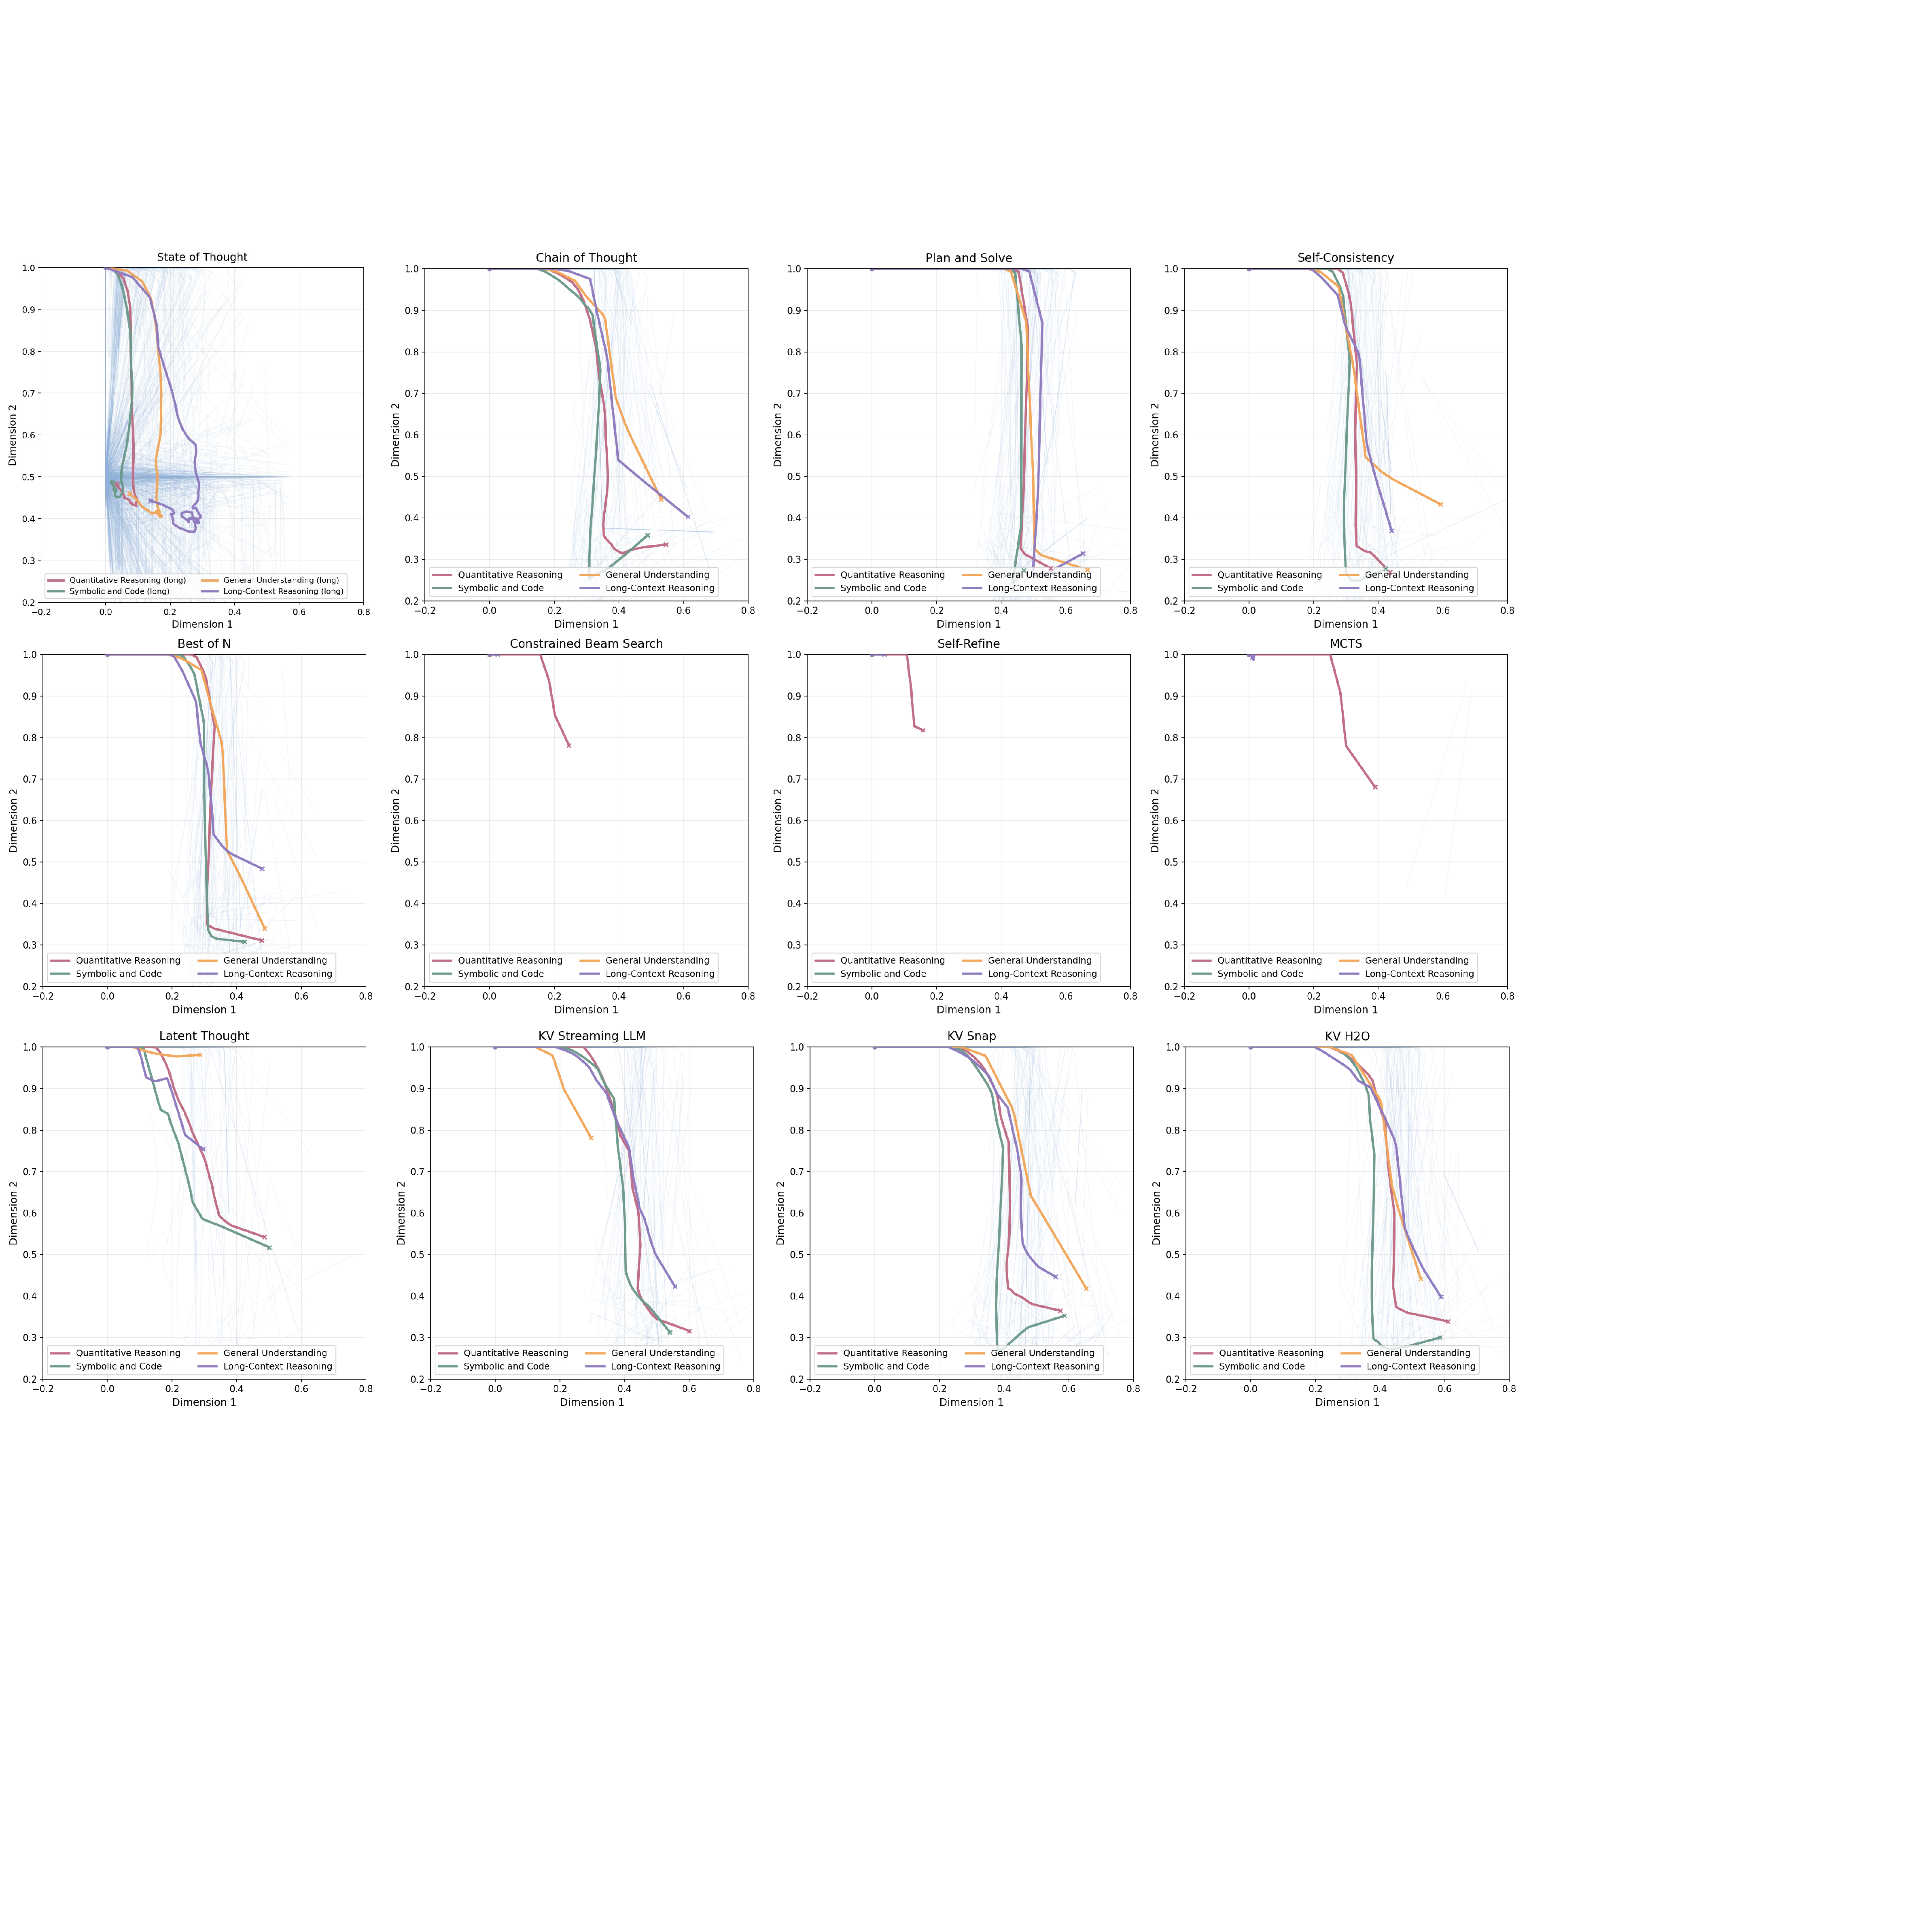
\includegraphics[width=1.0\textwidth]{figs/app_state_regimes.pdf}
\caption{
\textbf{Extended state-space trajectories across reasoning paradigms.}
This figure supplements the main-text trajectory view with additional paradigms and task categories.
}
\label{fig:app_state_regimes}
\end{figure*}

\paragraph{Interpretation.}
As shown in Figure~\ref{fig:app_state_regimes}, this analysis does not claim that each paradigm maps to a discrete symbolic state label.
Instead, it shows that the compact state \(m_t\) carries stable geometric structure: different paradigms trace distinguishable trajectory regions, while SoT occupies a broader and more adaptive regime rather than collapsing to a fixed externally scripted pattern.
The key insight is that SoT's gain is associated with controllable state coverage---reaching multiple useful regimes when needed---rather than with a single pre-committed reasoning template.

\subsection{State clusters, sparse memory, and stopping}
\label{app:cluster_ops}

We next extend the operator-level analysis of Sec.~\ref{sec:state_driven_activation}.
After aggregating SoT states across tasks, we cluster the observed \(m_t\) and summarize, for each cluster,
(i) its occupancy across task categories,
(ii) the average sparsity pattern of \(\mathcal{S}(y_{<t};m_t)\), and
(iii) the stop tendency induced by \(\mathcal{T}(m_t)\).
This links the geometry of the state space to concrete control behavior.

\begin{figure*}[t]
\centering
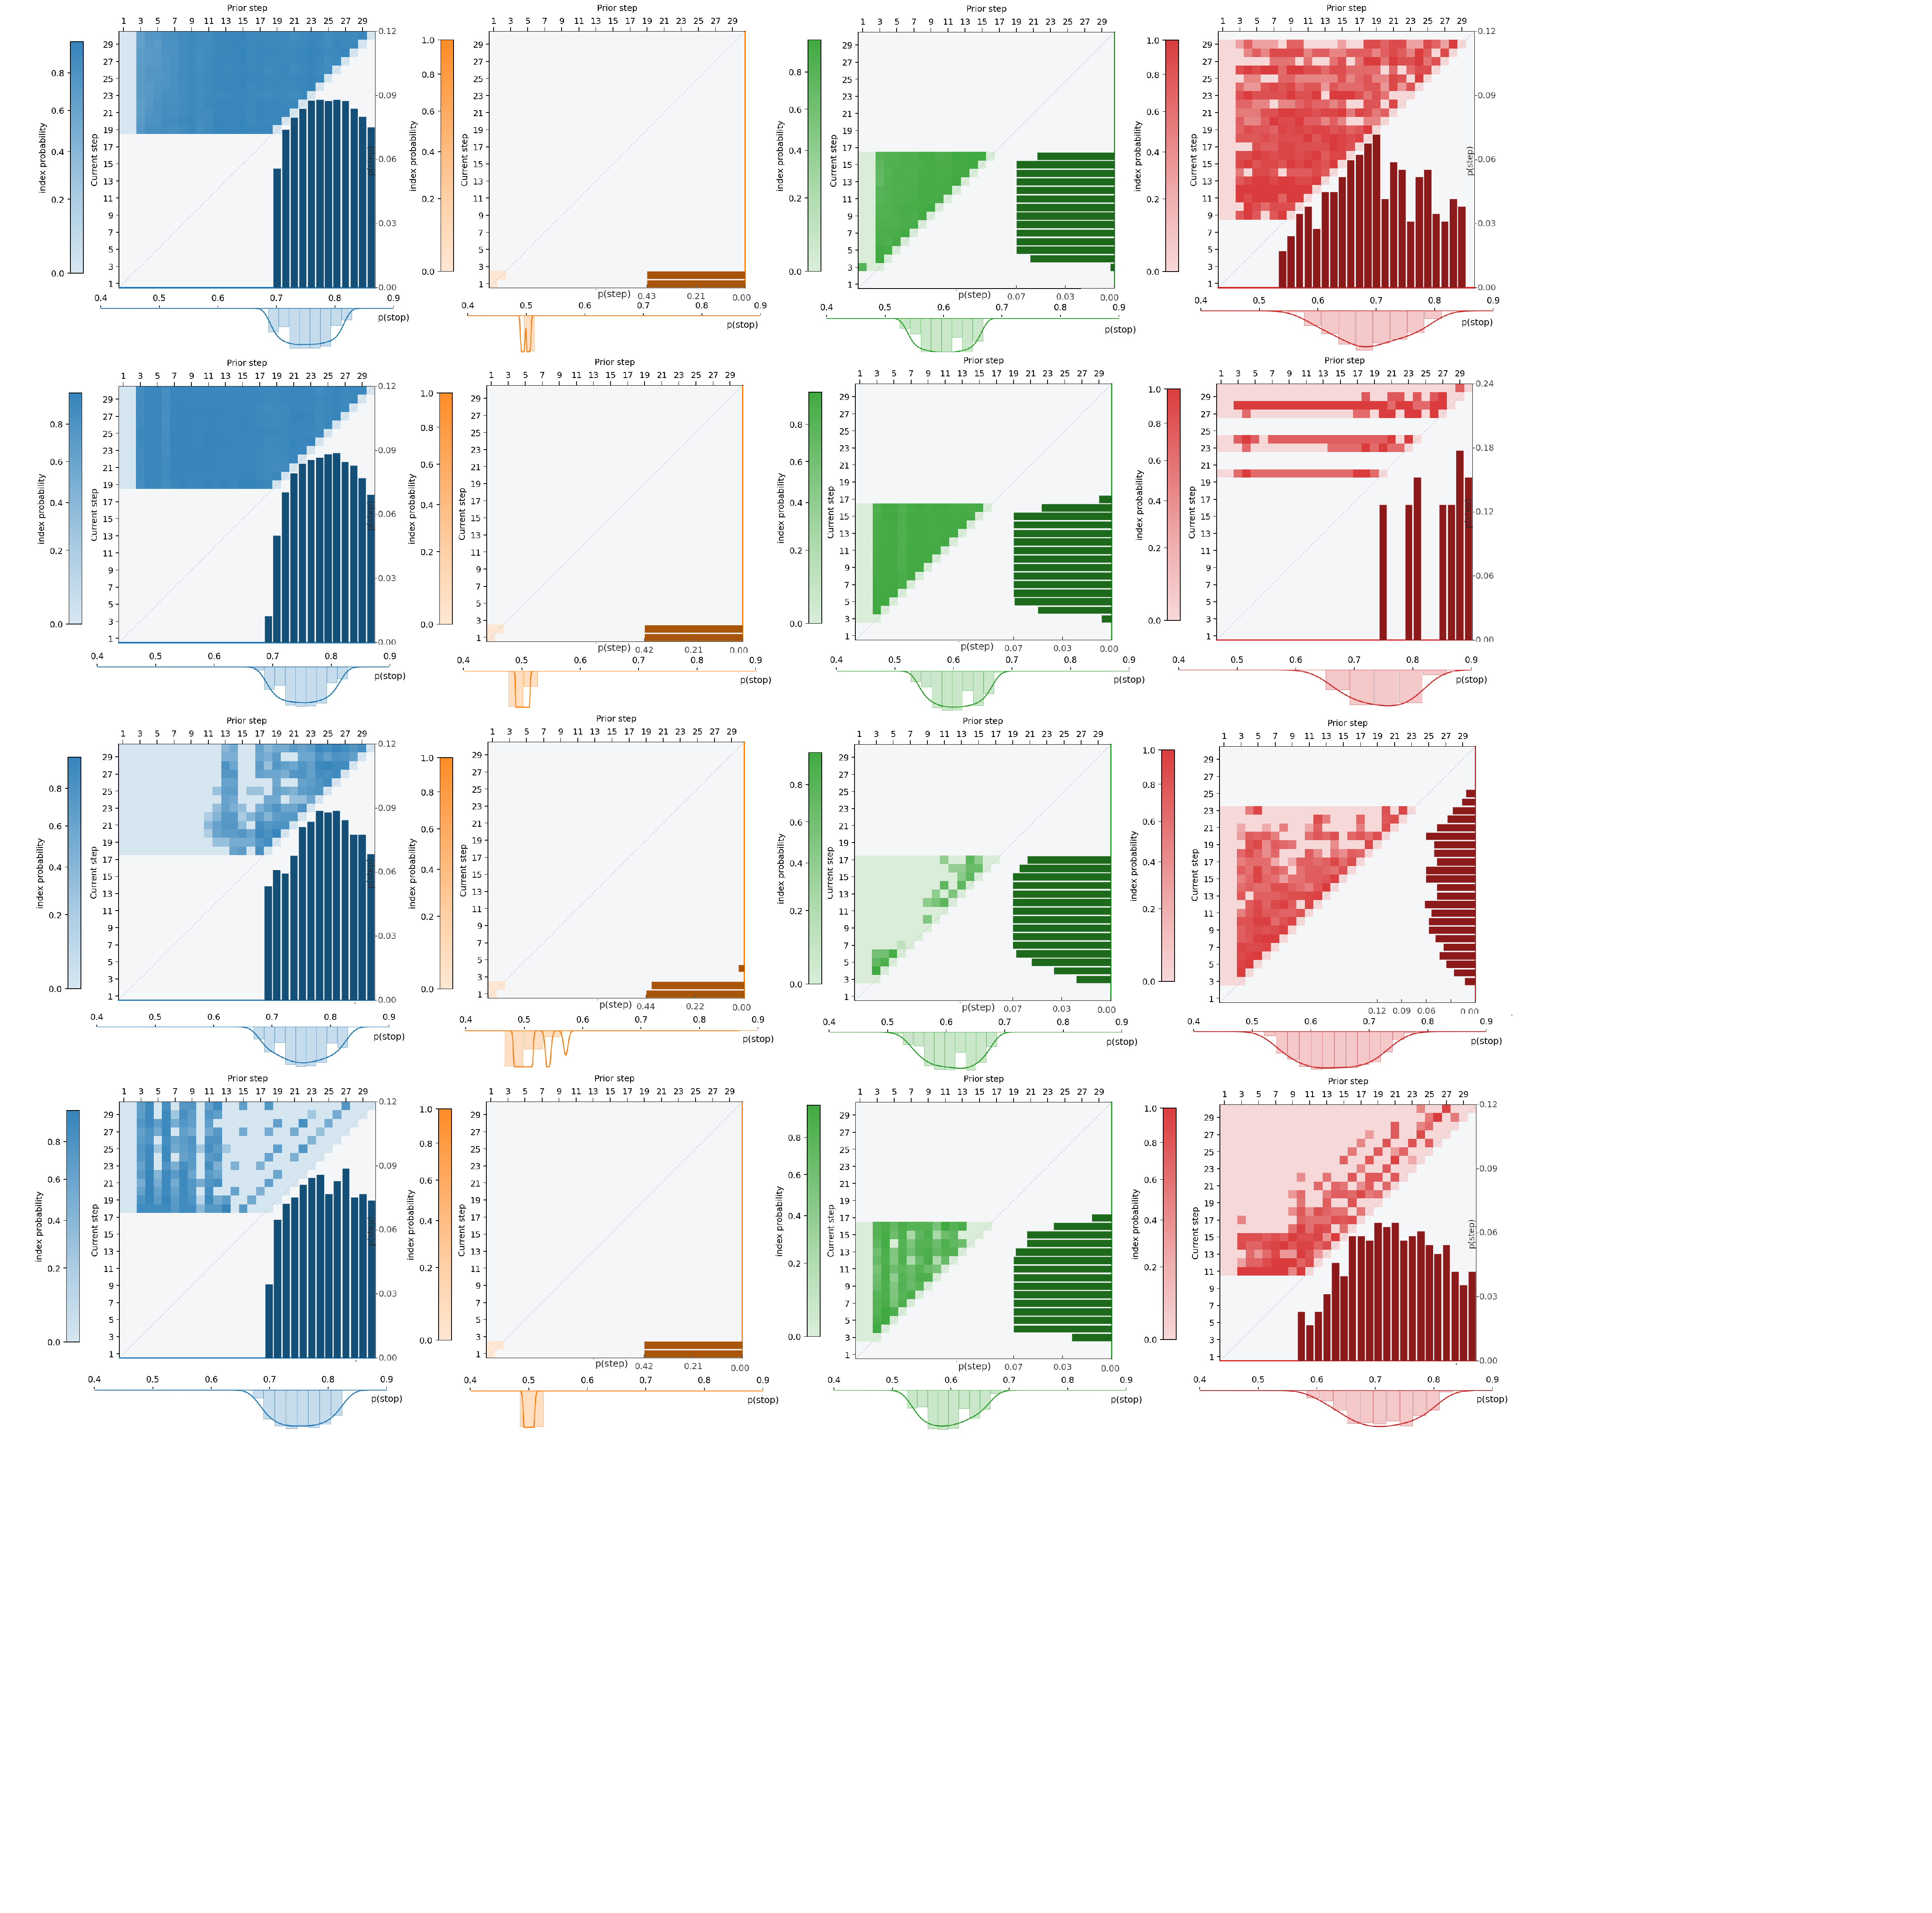
\includegraphics[width=1.0\textwidth]{figs/app_state_clusters.pdf}
\vspace{-4mm}
\caption{
\textbf{Clustered state regimes and operator profiles.}
}
\vspace{-4mm}
\label{fig:app_state_clusters}
\end{figure*}

\paragraph{Interpretation.}
Figure~\ref{fig:app_state_clusters} tests whether clustered states correspond to distinct control behavior, not just visual separability.
The observed cluster-specific sparsity and stop profiles indicate regime-dependent evidence organization and stopping, rather than generic recency bias, static compression, or a fixed-depth schedule.
This suggests that SoT's policy is conditionally compositional: the state first selects \emph{what} evidence remains active and then implicitly calibrates \emph{when} to terminate.

\subsection{Correct versus incorrect trajectories under internal and embedding-trajectory SoT}
\label{app:correct_wrong_traj}

Finally, we compare successful and unsuccessful trajectories under both the full SoT state and the SoT-Embed variant from Sec.~\ref{sec:endogenous_state} and Sec~\ref{sec:judge}.
For each of the four task categories, we aggregate trajectories by correctness and visualize the resulting state-space distributions.
We perform the same analysis twice:
once using the internal state derived from attention-side information transfer,
and once using features derived from the sentence-embedding trajectory (Appendix.~\ref{app:limitations_sot}).
This allows us to test whether the separation between healthy and unhealthy reasoning trajectories is preserved even when privileged internal access is removed.

\begin{figure*}[t]
\centering
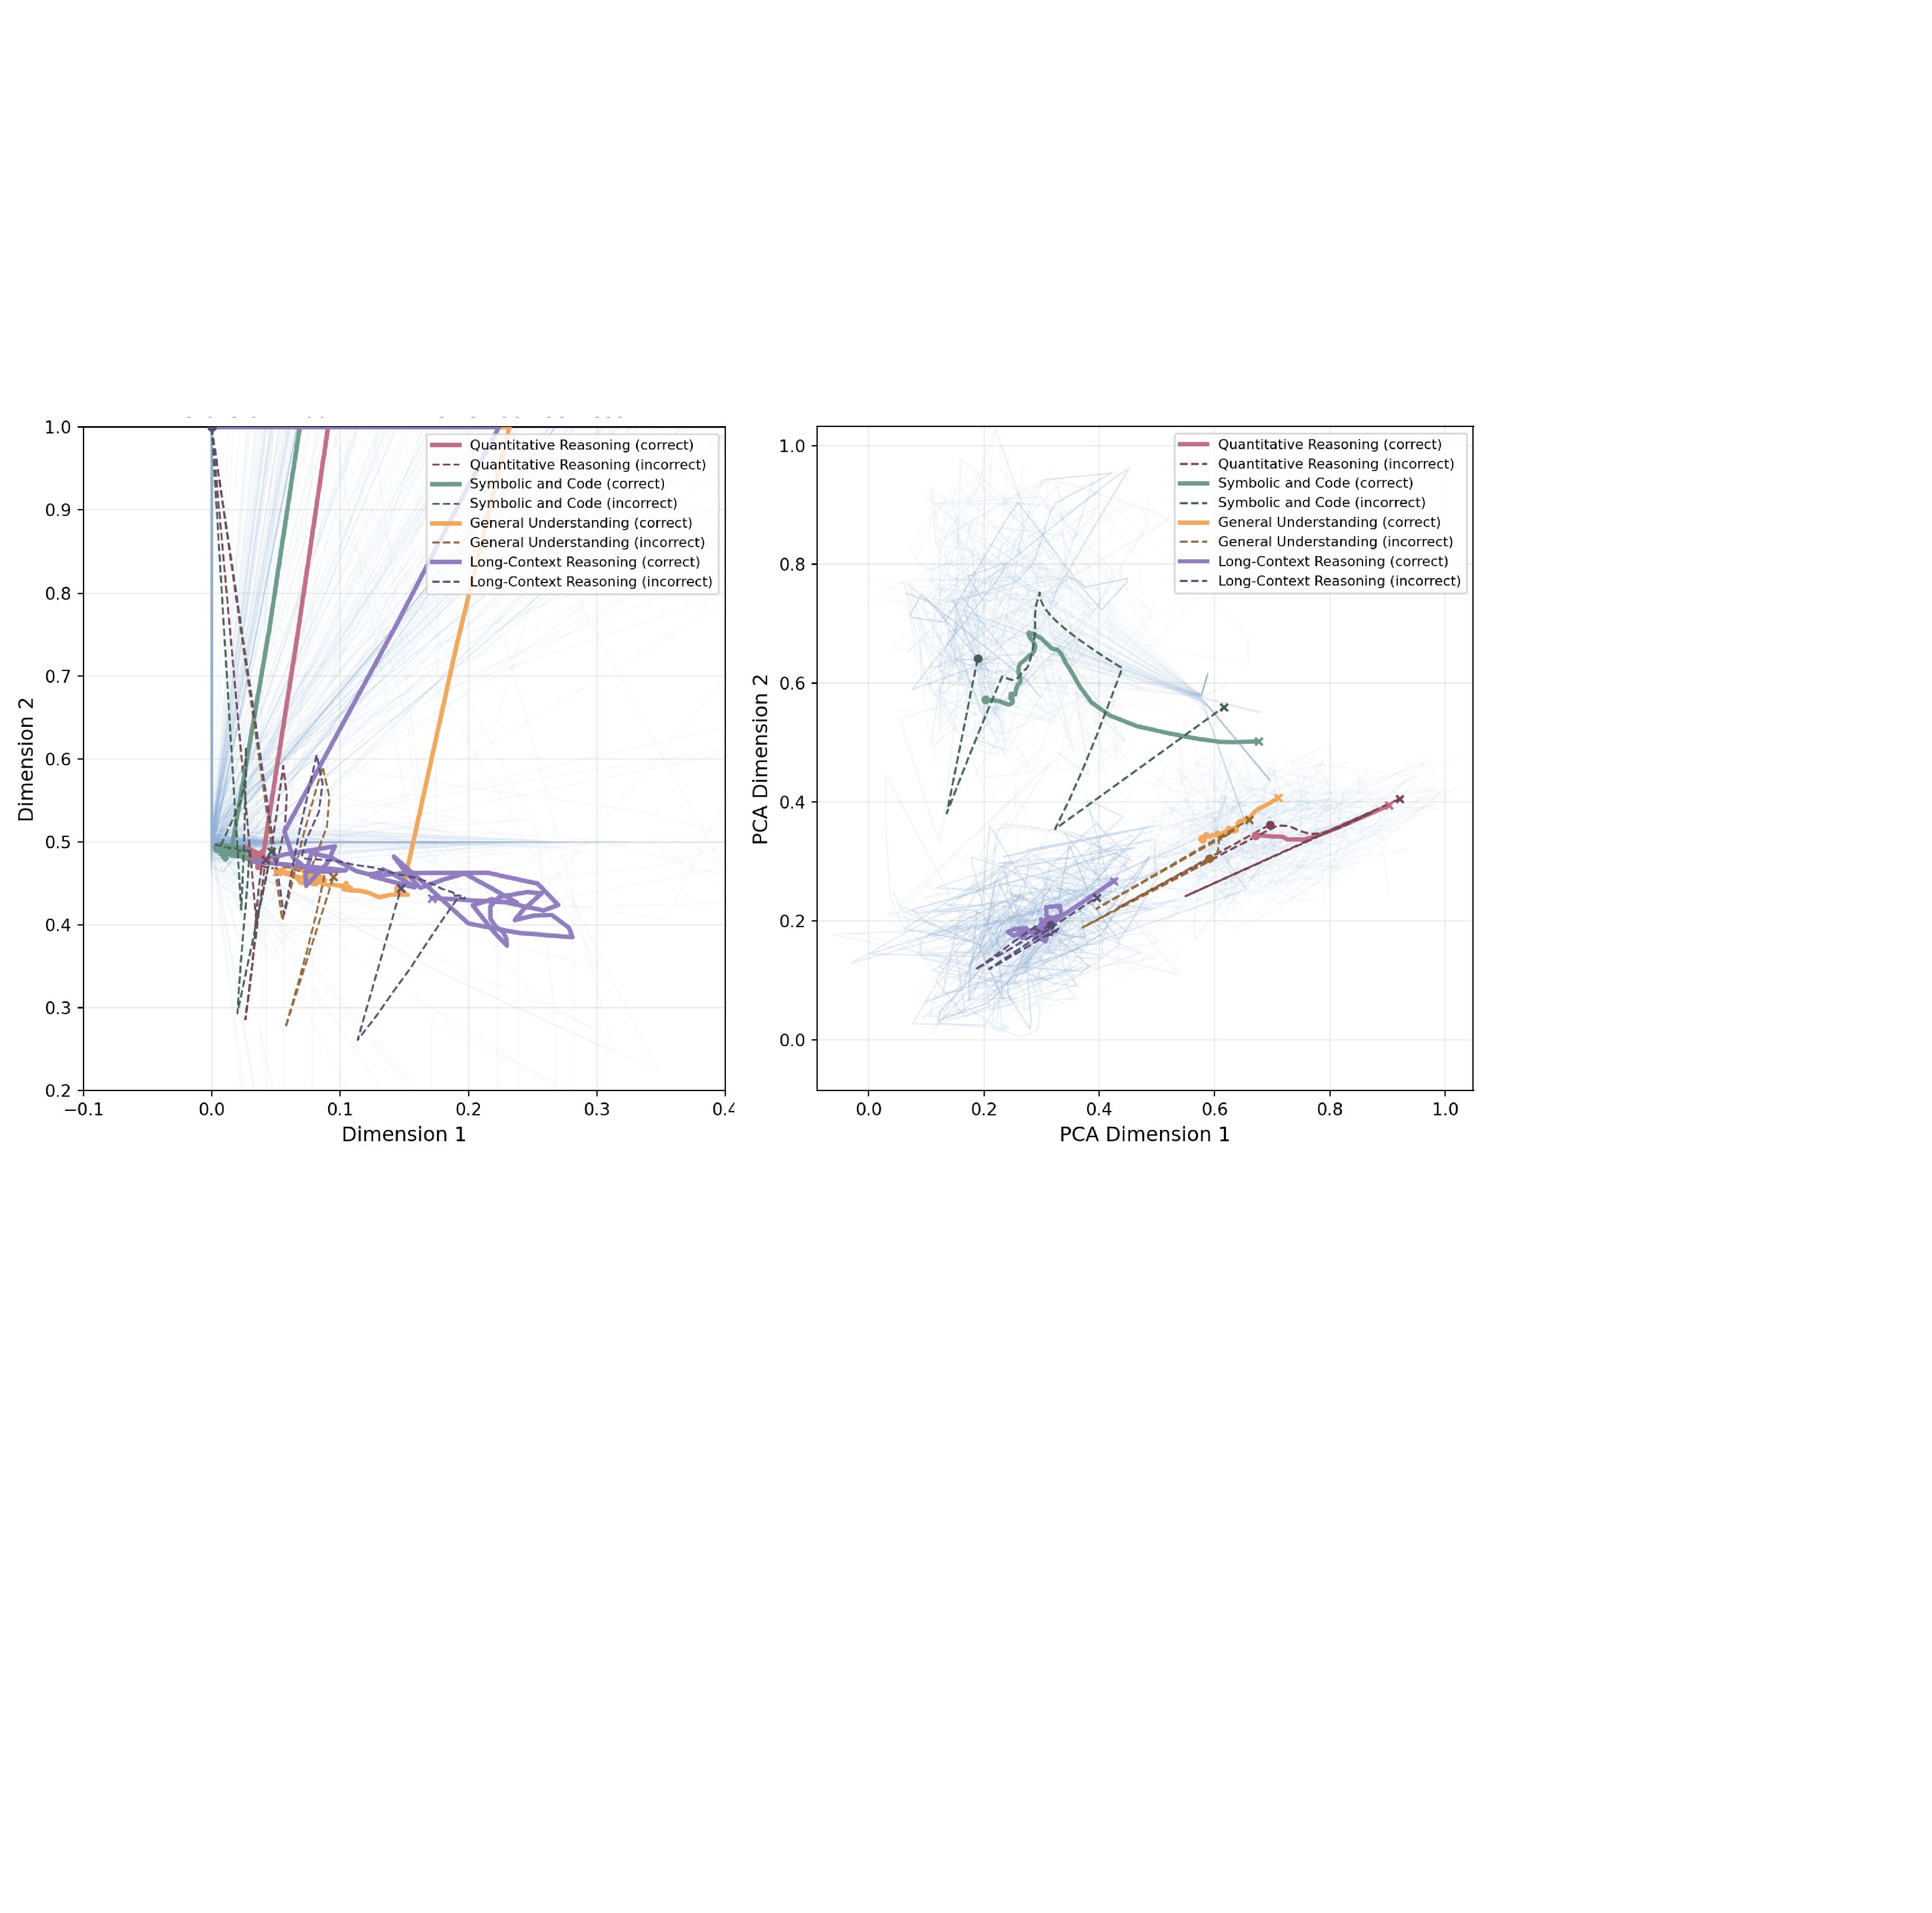
\includegraphics[width=1.0\textwidth]{figs/app_correct_incorrect.pdf}
\vspace{-5mm}
\caption{
\textbf{Correct and incorrect trajectory regimes under full-state and embedding-trajectory SoT.}
This figure compares successful and unsuccessful reasoning trajectories across all four task categories,
under both the internal-state SoT and SoT-Embed.
}
\vspace{-5mm}
\label{fig:app_correct_incorrect}
\end{figure*}

\paragraph{Interpretation.}
Figure~\ref{fig:app_correct_incorrect} serves two roles.
For full SoT, it links gains to trajectory quality by showing whether correct runs occupy more stable and favorable state regimes than incorrect runs.
For SoT-Embed, it tests whether this correct--incorrect separation persists under limited access; the preserved gap supports that SoT is a transferable trajectory-level principle rather than a privileged internal-state trick.
The practical insight is that trajectory-state separability can function as a lightweight health signal for reliability monitoring, even when white-box internals are unavailable.

\section{Additional Results}
\label{app:additional_results}

This section provides supplementary result tables and figures omitted from the main text for space.
Specifically, we provide backbone-specific main result tables, efficiency breakdown tables isolating tokens and latency, and limited-access variants expand the boundary studies.

\subsection{Additional backbone results}

Table~\ref{tab:app_main_qwen} and Table~\ref{tab:app_main_mixtral} report the full per-dataset accuracy results for the two LLM backbones not shown in the main text.
Two patterns are notable.
On Qwen2.5-14B, SoT achieves the best domain averages in QS (\(66.1\)), S\&C (\(76.8\)), and GU (\(81.4\)); the GU gain is especially clear, with all five GU datasets reaching the highest scores in the table (CSQA \(80.5\), StrQA \(75.0\), BoolQ \(86.8\), MMLU \(80.0\), RACE \(86.0\)).
On Mixtral-8x7B, SoT is near-best in QS (\(46.3\), close to \(46.4\)) and leads clearly in S\&C (\(51.7\)), GU (\(72.6\)), and LCR (\(23.5\)), indicating that the same state-conditioned control remains effective across substantially different backbone characteristics.
Taken together, these cross-backbone results support a mechanism-level claim: SoT's advantage is not tied to one architecture or one dataset family, but to a transferable control principle that improves diverse reasoning regimes under heterogeneous model priors.

\begin{table*}[!t]
\centering
%\vspace{-4mm}
\caption{\textbf{Main results on Qwen2.5-14B (accuracy, \%).}}
\label{tab:app_main_qwen}
\vspace{-2mm}
\footnotesize
{\setlength{\tabcolsep}{1.3pt}%
\setlength{\aboverulesep}{0pt}%
\setlength{\belowrulesep}{0pt}%
\setlength{\extrarowheight}{1.43pt}%
\renewcommand{\arraystretch}{0.823}%
\renewcommand{\tabularxcolumn}[1]{m{#1}}%
\begin{tabularx}{\linewidth}{@{} >{\centering\arraybackslash}p{1.65cm} >{\centering\arraybackslash}m{1.28cm} !{\vrule width 0.4pt} >{\centering\arraybackslash}X >{\centering\arraybackslash}X >{\centering\arraybackslash}X >{\centering\arraybackslash}m{3.1em} >{\centering\arraybackslash}X >{\centering\arraybackslash}X >{\centering\arraybackslash}X >{\centering\arraybackslash}X >{\centering\arraybackslash}X >{\centering\arraybackslash}m{3.1em} @{}}
\toprule
\multirow{2}{=}{\centering\textbf{Category}} & \multirow{2}{=}{\centering\textbf{Method}}
& \multicolumn{4}{>{\cellcolor[HTML]{E3F2FD}}c!{\vrule width 1pt}}{\textbf{Quantitative Reasoning}}
& \multicolumn{6}{>{\cellcolor[HTML]{E3F2FD}}c}{\textbf{Symbolic and Code}} \\
&
& {\small\textbf{GSM}} & {\small\textbf{MATH}} & {\small\textbf{DROP}} & \multicolumn{1}{>{\centering\arraybackslash}m{3.1em}!{\vrule width 1pt}}{\small\textbf{avg.}}
& {\small\textbf{FOL}} & {\small\textbf{PW}} & {\small\textbf{BBH}} & {\small\textbf{HE}} & {\small\textbf{MBPP}} & \multicolumn{1}{>{\centering\arraybackslash}m{3.1em}}{\small\textbf{avg.}} \\
\midrule
\multirow{7}{=}{\centering Reasoning\\Paradigm} & CoT & \cellcolor[HTML]{FFD4D3}{94.4} & \cellcolor[HTML]{FFD4D3}{77.5} & 1.9 & \multicolumn{1}{>{\centering\arraybackslash}m{3.1em}!{\vrule width 1pt}}{\cellcolor[HTML]{EAECEF}{65.6}} & 0.0 & 55.5 & 84.0 & \cellcolor[HTML]{FCE4D5}{75.0} & \cellcolor[HTML]{FFD4D3}{66.0} & \multicolumn{1}{>{\centering\arraybackslash}m{3.1em}}{\cellcolor[HTML]{EAECEF}{49.9}} \\
 & PS & 88.0 & 51.5 & 2.1 & \multicolumn{1}{>{\centering\arraybackslash}m{3.1em}!{\vrule width 1pt}}{\cellcolor[HTML]{EAECEF}{54.4}} & 0.5 & 65.5 & \cellcolor[HTML]{FFD4D3}{92.0} & 50.0 & 47.2 & \multicolumn{1}{>{\centering\arraybackslash}m{3.1em}}{\cellcolor[HTML]{EAECEF}{49.6}} \\
 & SR & 92.0 & 68.2 & \cellcolor[HTML]{FFFCE0}{17.6} & \multicolumn{1}{>{\centering\arraybackslash}m{3.1em}!{\vrule width 1pt}}{\cellcolor[HTML]{EAECEF}{65.5}} & 61.1 & 83.4 & 79.0 & 60.0 & 50.4 & \multicolumn{1}{>{\centering\arraybackslash}m{3.1em}}{\cellcolor[HTML]{EAECEF}{68.1}} \\
 & SC & \cellcolor[HTML]{FFFCE0}{92.8} & 61.0 & 1.9 & \multicolumn{1}{>{\centering\arraybackslash}m{3.1em}!{\vrule width 1pt}}{\cellcolor[HTML]{EAECEF}{59.5}} & 0.5 & 59.5 & \cellcolor[HTML]{FFFCE0}{87.0} & 55.0 & 48.8 & \multicolumn{1}{>{\centering\arraybackslash}m{3.1em}}{\cellcolor[HTML]{EAECEF}{47.2}} \\
 & BoN & \cellcolor[HTML]{FFFCE0}{92.8} & 61.0 & 1.9 & \multicolumn{1}{>{\centering\arraybackslash}m{3.1em}!{\vrule width 1pt}}{\cellcolor[HTML]{EAECEF}{59.5}} & 1.0 & 59.5 & \cellcolor[HTML]{FFFCE0}{87.0} & 55.0 & 48.8 & \multicolumn{1}{>{\centering\arraybackslash}m{3.1em}}{\cellcolor[HTML]{EAECEF}{47.3}} \\
 & CB & 60.0 & 41.2 & \cellcolor[HTML]{FFD4D3}{30.8} & \multicolumn{1}{>{\centering\arraybackslash}m{3.1em}!{\vrule width 1pt}}{\cellcolor[HTML]{EAECEF}{46.4}} & \cellcolor[HTML]{FFFCE0}{62.1} & \cellcolor[HTML]{FFFCE0}{85.0} & 51.0 & 50.0 & 60.8 & \multicolumn{1}{>{\centering\arraybackslash}m{3.1em}}{\cellcolor[HTML]{EAECEF}{69.8}} \\
 & MCTS & 66.2 & 50.0 & \cellcolor[HTML]{FCE4D5}{19.3} & \multicolumn{1}{>{\centering\arraybackslash}m{3.1em}!{\vrule width 1pt}}{\cellcolor[HTML]{EAECEF}{49.1}} & \cellcolor[HTML]{FCE4D5}{63.1} & \cellcolor[HTML]{FFD4D3}{88.5} & 53.0 & 60.0 & \cellcolor[HTML]{FCE4D5}{63.6} & \multicolumn{1}{>{\centering\arraybackslash}m{3.1em}}{\cellcolor[HTML]{EAECEF}{72.6}} \\
\midrule
\multirow{3}{=}{\centering Memory-Oriented} & H2O & 92.6 & 67.0 & 2.6 & \multicolumn{1}{>{\centering\arraybackslash}m{3.1em}!{\vrule width 1pt}}{\cellcolor[HTML]{EAECEF}{61.6}} & 0.5 & 14.8 & 81.0 & 72.8 & 45.2 & \multicolumn{1}{>{\centering\arraybackslash}m{3.1em}}{\cellcolor[HTML]{EAECEF}{33.4}} \\
 & SNAP & \cellcolor[HTML]{FFFCE0}{92.8} & 66.5 & 2.7 & \multicolumn{1}{>{\centering\arraybackslash}m{3.1em}!{\vrule width 1pt}}{\cellcolor[HTML]{EAECEF}{61.5}} & 2.0 & 13.0 & 83.0 & \cellcolor[HTML]{FFFCE0}{73.5} & 44.0 & \multicolumn{1}{>{\centering\arraybackslash}m{3.1em}}{\cellcolor[HTML]{EAECEF}{33.1}} \\
 & STREAM & 78.0 & 45.8 & 1.8 & \multicolumn{1}{>{\centering\arraybackslash}m{3.1em}!{\vrule width 1pt}}{\cellcolor[HTML]{EAECEF}{48.2}} & 5.9 & 19.5 & 3.0 & 68.4 & 3.2 & \multicolumn{1}{>{\centering\arraybackslash}m{3.1em}}{\cellcolor[HTML]{EAECEF}{19.1}} \\
\midrule
Latent & COCO & \cellcolor[HTML]{FCE4D5}{93.6} & \cellcolor[HTML]{FCE4D5}{74.8} & 2.8 & \multicolumn{1}{>{\centering\arraybackslash}m{3.1em}!{\vrule width 1pt}}{\cellcolor[HTML]{EAECEF}{64.6}} & 2.5 & 40.5 & 75.0 & 71.2 & 60.0 & \multicolumn{1}{>{\centering\arraybackslash}m{3.1em}}{\cellcolor[HTML]{EAECEF}{45.6}} \\
\midrule
RL-Based & GRPO\textsuperscript{\raisebox{-0.08ex}{\scriptsize\kern0.06em\textbf{+}}} & 0.6 & 5.0 & 0.0 & \multicolumn{1}{>{\centering\arraybackslash}m{3.1em}!{\vrule width 1pt}}{\cellcolor[HTML]{EAECEF}{1.9}} & 3.4 & 3.0 & 5.0 & 58.7 & 0.0 & \multicolumn{1}{>{\centering\arraybackslash}m{3.1em}}{\cellcolor[HTML]{EAECEF}{10.8}} \\
\midrule
Ours & \textbf{SoT} & \textbf{91.8} & \cellcolor[HTML]{FFFCE0}{\textbf{72.2}} & \textbf{15.1} & \multicolumn{1}{>{\centering\arraybackslash}m{3.1em}!{\vrule width 1pt}}{\cellcolor[HTML]{EAECEF}{\underline{\textbf{66.1}}}} & \cellcolor[HTML]{FFD4D3}{\textbf{66.5}} & \cellcolor[HTML]{FCE4D5}{\textbf{87.8}} & \cellcolor[HTML]{FCE4D5}{\textbf{91.0}} & \cellcolor[HTML]{FFD4D3}{\textbf{75.6}} & \cellcolor[HTML]{FFFCE0}{\textbf{62.8}} & \multicolumn{1}{>{\centering\arraybackslash}m{3.1em}}{\cellcolor[HTML]{EAECEF}{\underline{\textbf{76.8}}}} \\
\midrule\end{tabularx}\par\addvspace{0.35ex}}%
{\setlength{\tabcolsep}{1.3pt}%
\setlength{\aboverulesep}{0pt}%
\setlength{\belowrulesep}{0pt}%
\setlength{\extrarowheight}{1.43pt}%
\renewcommand{\arraystretch}{0.823}%
\renewcommand{\tabularxcolumn}[1]{m{#1}}%
\begin{tabularx}{\linewidth}{@{} >{\centering\arraybackslash}p{1.65cm} >{\centering\arraybackslash}m{1.28cm} !{\vrule width 0.4pt} >{\centering\arraybackslash}X >{\centering\arraybackslash}X >{\centering\arraybackslash}X >{\centering\arraybackslash}X >{\centering\arraybackslash}X >{\centering\arraybackslash}m{3.1em} >{\centering\arraybackslash}X >{\centering\arraybackslash}X >{\centering\arraybackslash}X >{\centering\arraybackslash}m{3.1em} @{}}
\multirow{2}{=}{\centering\textbf{Category}} & \multirow{2}{=}{\centering\textbf{Method}}
& \multicolumn{6}{>{\cellcolor[HTML]{E3F2FD}}c!{\vrule width 1pt}}{\textbf{General Understanding}}
& \multicolumn{4}{>{\cellcolor[HTML]{E3F2FD}}c}{\textbf{Long-Context Reasoning}} \\
&
& {\small\textbf{CSQA}} & {\small\textbf{StrQA}} & {\small\textbf{BoolQ}} & {\small\textbf{MMLU}} & {\small\textbf{RACE}} & \multicolumn{1}{>{\centering\arraybackslash}m{3.1em}!{\vrule width 1pt}}{\small\textbf{avg.}}
& {\small\textbf{HQA}} & {\small\textbf{NarQA}} & {\small\textbf{LB}} & \multicolumn{1}{>{\centering\arraybackslash}m{3.1em}}{\small\textbf{avg.}} \\
\midrule
\multirow{7}{=}{\centering Reasoning\\Paradigm} & CoT & 42.8 & 51.2 & 61.5 & 39.8 & 36.8 & \multicolumn{1}{>{\centering\arraybackslash}m{3.1em}!{\vrule width 1pt}}{\cellcolor[HTML]{EAECEF}{46.6}} & 2.0 & 4.6 & 18.4 & \multicolumn{1}{>{\centering\arraybackslash}m{3.1em}}{\cellcolor[HTML]{EAECEF}{5.7}} \\
 & PS & 58.0 & 58.4 & 42.0 & 48.6 & 40.2 & \multicolumn{1}{>{\centering\arraybackslash}m{3.1em}!{\vrule width 1pt}}{\cellcolor[HTML]{EAECEF}{49.9}} & 2.5 & 5.6 & 23.9 & \multicolumn{1}{>{\centering\arraybackslash}m{3.1em}}{\cellcolor[HTML]{EAECEF}{7.3}} \\
 & SR & \cellcolor[HTML]{FCE4D5}{75.0} & \cellcolor[HTML]{FCE4D5}{71.6} & 81.8 & \cellcolor[HTML]{FCE4D5}{74.0} & 63.4 & \multicolumn{1}{>{\centering\arraybackslash}m{3.1em}!{\vrule width 1pt}}{\cellcolor[HTML]{EAECEF}{73.7}} & 16.3 & 25.0 & \cellcolor[HTML]{FFD4D3}{30.8} & \multicolumn{1}{>{\centering\arraybackslash}m{3.1em}}{\cellcolor[HTML]{EAECEF}{22.0}} \\
 & SC & 40.2 & 55.8 & 61.8 & 38.6 & 48.6 & \multicolumn{1}{>{\centering\arraybackslash}m{3.1em}!{\vrule width 1pt}}{\cellcolor[HTML]{EAECEF}{48.5}} & 2.0 & 4.4 & 22.5 & \multicolumn{1}{>{\centering\arraybackslash}m{3.1em}}{\cellcolor[HTML]{EAECEF}{6.3}} \\
 & BoN & 40.2 & 55.6 & 61.8 & 38.6 & 49.2 & \multicolumn{1}{>{\centering\arraybackslash}m{3.1em}!{\vrule width 1pt}}{\cellcolor[HTML]{EAECEF}{48.5}} & 2.0 & 4.4 & 16.4 & \multicolumn{1}{>{\centering\arraybackslash}m{3.1em}}{\cellcolor[HTML]{EAECEF}{5.3}} \\
 & CB & 71.0 & \cellcolor[HTML]{FFFCE0}{70.2} & \cellcolor[HTML]{FFFCE0}{84.5} & \cellcolor[HTML]{FFFCE0}{67.8} & \cellcolor[HTML]{FFFCE0}{63.8} & \multicolumn{1}{>{\centering\arraybackslash}m{3.1em}!{\vrule width 1pt}}{\cellcolor[HTML]{EAECEF}{71.7}} & \cellcolor[HTML]{FFD4D3}{25.8} & \cellcolor[HTML]{FFD4D3}{33.5} & 26.3 & \multicolumn{1}{>{\centering\arraybackslash}m{3.1em}}{\cellcolor[HTML]{EAECEF}{\underline{28.8}}} \\
 & MCTS & \cellcolor[HTML]{FFFCE0}{71.2} & 69.4 & \cellcolor[HTML]{FCE4D5}{85.8} & 65.8 & 62.6 & \multicolumn{1}{>{\centering\arraybackslash}m{3.1em}!{\vrule width 1pt}}{\cellcolor[HTML]{EAECEF}{71.1}} & \cellcolor[HTML]{FFFCE0}{17.0} & \cellcolor[HTML]{FCE4D5}{29.0} & \cellcolor[HTML]{FCE4D5}{28.5} & \multicolumn{1}{>{\centering\arraybackslash}m{3.1em}}{\cellcolor[HTML]{EAECEF}{23.5}} \\
\midrule
\multirow{3}{=}{\centering Memory-Oriented} & H2O & 41.8 & 47.2 & 61.5 & 37.0 & 24.7 & \multicolumn{1}{>{\centering\arraybackslash}m{3.1em}!{\vrule width 1pt}}{\cellcolor[HTML]{EAECEF}{43.1}} & 2.0 & 2.0 & 0.0 & \multicolumn{1}{>{\centering\arraybackslash}m{3.1em}}{\cellcolor[HTML]{EAECEF}{1.7}} \\
 & SNAP & 41.8 & 47.2 & 61.0 & 37.4 & 27.0 & \multicolumn{1}{>{\centering\arraybackslash}m{3.1em}!{\vrule width 1pt}}{\cellcolor[HTML]{EAECEF}{43.4}} & 2.0 & 2.0 & 0.0 & \multicolumn{1}{>{\centering\arraybackslash}m{3.1em}}{\cellcolor[HTML]{EAECEF}{1.7}} \\
 & STREAM & 39.8 & 46.2 & 52.8 & 33.2 & 0.0 & \multicolumn{1}{>{\centering\arraybackslash}m{3.1em}!{\vrule width 1pt}}{\cellcolor[HTML]{EAECEF}{36.1}} & 2.4 & 0.0 & 0.0 & \multicolumn{1}{>{\centering\arraybackslash}m{3.1em}}{\cellcolor[HTML]{EAECEF}{1.1}} \\
\midrule
Latent & COCO & 49.0 & 45.5 & 61.8 & 53.6 & \cellcolor[HTML]{FCE4D5}{65.7} & \multicolumn{1}{>{\centering\arraybackslash}m{3.1em}!{\vrule width 1pt}}{\cellcolor[HTML]{EAECEF}{54.5}} & 2.3 & 7.4 & 25.3 & \multicolumn{1}{>{\centering\arraybackslash}m{3.1em}}{\cellcolor[HTML]{EAECEF}{8.0}} \\
\midrule
RL-Based & GRPO\textsuperscript{\raisebox{-0.08ex}{\scriptsize\kern0.06em\textbf{+}}} & 10.0 & 5.8 & 5.2 & 8.2 & 12.7 & \multicolumn{1}{>{\centering\arraybackslash}m{3.1em}!{\vrule width 1pt}}{\cellcolor[HTML]{EAECEF}{8.2}} & 0.1 & 0.1 & 0.3 & \multicolumn{1}{>{\centering\arraybackslash}m{3.1em}}{\cellcolor[HTML]{EAECEF}{0.1}} \\
\midrule
Ours & \textbf{SoT} & \cellcolor[HTML]{FFD4D3}{\textbf{80.5}} & \cellcolor[HTML]{FFD4D3}{\textbf{75.0}} & \cellcolor[HTML]{FFD4D3}{\textbf{86.8}} & \cellcolor[HTML]{FFD4D3}{\textbf{80.0}} & \cellcolor[HTML]{FFD4D3}{\textbf{86.0}} & \multicolumn{1}{>{\centering\arraybackslash}m{3.1em}!{\vrule width 1pt}}{\cellcolor[HTML]{EAECEF}{\underline{\textbf{81.4}}}} & \cellcolor[HTML]{FCE4D5}{\textbf{24.2}} & \cellcolor[HTML]{FFFCE0}{\textbf{25.4}} & \cellcolor[HTML]{FFFCE0}{\textbf{27.3}} & \multicolumn{1}{>{\centering\arraybackslash}m{3.1em}}{\cellcolor[HTML]{EAECEF}{\textbf{25.2}}} \\
\bottomrule\end{tabularx}}%

\vspace{-2mm}
\end{table*}

\begin{table*}[!t]
\centering
\caption{\textbf{Main results on Mixtral-8x7B (accuracy, \%).}}
\label{tab:app_main_mixtral}
\vspace{-2mm}
\footnotesize
{\setlength{\tabcolsep}{1.3pt}%
\setlength{\aboverulesep}{0pt}%
\setlength{\belowrulesep}{0pt}%
\setlength{\extrarowheight}{1.43pt}%
\renewcommand{\arraystretch}{0.823}%
\renewcommand{\tabularxcolumn}[1]{m{#1}}%
\begin{tabularx}{\linewidth}{@{} >{\centering\arraybackslash}p{1.65cm} >{\centering\arraybackslash}m{1.28cm} !{\vrule width 0.4pt} >{\centering\arraybackslash}X >{\centering\arraybackslash}X >{\centering\arraybackslash}X >{\centering\arraybackslash}m{3.1em} >{\centering\arraybackslash}X >{\centering\arraybackslash}X >{\centering\arraybackslash}X >{\centering\arraybackslash}X >{\centering\arraybackslash}X >{\centering\arraybackslash}m{3.1em} @{}}
\toprule
\multirow{2}{=}{\centering\textbf{Category}} & \multirow{2}{=}{\centering\textbf{Method}}
& \multicolumn{4}{>{\cellcolor[HTML]{E3F2FD}}c!{\vrule width 1pt}}{\textbf{Quantitative Reasoning}}
& \multicolumn{6}{>{\cellcolor[HTML]{E3F2FD}}c}{\textbf{Symbolic and Code}} \\
&
& {\small\textbf{GSM}} & {\small\textbf{MATH}} & {\small\textbf{DROP}} & \multicolumn{1}{>{\centering\arraybackslash}m{3.1em}!{\vrule width 1pt}}{\small\textbf{avg.}}
& {\small\textbf{FOL}} & {\small\textbf{PW}} & {\small\textbf{BBH}} & {\small\textbf{HE}} & {\small\textbf{MBPP}} & \multicolumn{1}{>{\centering\arraybackslash}m{3.1em}}{\small\textbf{avg.}} \\
\midrule
\multirow{7}{=}{\centering Reasoning\\Paradigm}
 & CoT & 64.8 & 41.5 & 9.9 & \multicolumn{1}{>{\centering\arraybackslash}m{3.1em}!{\vrule width 1pt}}{\cellcolor[HTML]{EAECEF}{43.3}} & 23.2 & 43.0 & 47.0 & \cellcolor[HTML]{FFFCE0}{20.0} & \cellcolor[HTML]{FFFCE0}{40.4} & \multicolumn{1}{>{\centering\arraybackslash}m{3.1em}}{\cellcolor[HTML]{EAECEF}{38.1}} \\
 & PS & 60.6 & 35.8 & \cellcolor[HTML]{FCE4D5}{10.6} & \multicolumn{1}{>{\centering\arraybackslash}m{3.1em}!{\vrule width 1pt}}{\cellcolor[HTML]{EAECEF}{39.8}} & 12.8 & 38.2 & 52.0 & \cellcolor[HTML]{FCE4D5}{25.0} & \cellcolor[HTML]{FCE4D5}{42.4} & \multicolumn{1}{>{\centering\arraybackslash}m{3.1em}}{\cellcolor[HTML]{EAECEF}{35.1}} \\
 & SR & 49.2 & 37.8 & 9.7 & \multicolumn{1}{>{\centering\arraybackslash}m{3.1em}!{\vrule width 1pt}}{\cellcolor[HTML]{EAECEF}{35.5}} & 27.6 & 54.5 & 51.0 & 15.0 & 32.0 & \multicolumn{1}{>{\centering\arraybackslash}m{3.1em}}{\cellcolor[HTML]{EAECEF}{41.9}} \\
 & SC & \cellcolor[HTML]{FFD4D3}{69.8} & \cellcolor[HTML]{FFFCE0}{43.0} & 9.8 & \multicolumn{1}{>{\centering\arraybackslash}m{3.1em}!{\vrule width 1pt}}{\cellcolor[HTML]{EAECEF}{45.9}} & 25.6 & 45.2 & \cellcolor[HTML]{FCE4D5}{56.0} & 20.0 & 37.2 & \multicolumn{1}{>{\centering\arraybackslash}m{3.1em}}{\cellcolor[HTML]{EAECEF}{39.7}} \\
 & BoN & \cellcolor[HTML]{FFFCE0}{69.0} & \cellcolor[HTML]{FFD4D3}{46.0} & 9.3 & \multicolumn{1}{>{\centering\arraybackslash}m{3.1em}!{\vrule width 1pt}}{\cellcolor[HTML]{EAECEF}{\underline{46.4}}} & 23.6 & 49.0 & \cellcolor[HTML]{FFD4D3}{59.0} & 15.0 & 38.0 & \multicolumn{1}{>{\centering\arraybackslash}m{3.1em}}{\cellcolor[HTML]{EAECEF}{41.2}} \\
 & CB & 50.0 & 30.2 & \cellcolor[HTML]{FFFCE0}{10.1} & \multicolumn{1}{>{\centering\arraybackslash}m{3.1em}!{\vrule width 1pt}}{\cellcolor[HTML]{EAECEF}{33.4}} & \cellcolor[HTML]{FCE4D5}{48.3} & \cellcolor[HTML]{FCE4D5}{60.5} & 39.0 & 10.0 & 34.4 & \multicolumn{1}{>{\centering\arraybackslash}m{3.1em}}{\cellcolor[HTML]{EAECEF}{48.0}} \\
 & MCTS & 45.6 & 26.8 & 8.0 & \multicolumn{1}{>{\centering\arraybackslash}m{3.1em}!{\vrule width 1pt}}{\cellcolor[HTML]{EAECEF}{29.9}} & \cellcolor[HTML]{FFD4D3}{50.7} & \cellcolor[HTML]{FFFCE0}{57.2} & 39.0 & 20.0 & 38.4 & \multicolumn{1}{>{\centering\arraybackslash}m{3.1em}}{\cellcolor[HTML]{EAECEF}{48.4}} \\
\midrule
\multirow{3}{=}{\centering Memory-Oriented}
 & H2O & 65.2 & 43.0 & 9.4 & \multicolumn{1}{>{\centering\arraybackslash}m{3.1em}!{\vrule width 1pt}}{\cellcolor[HTML]{EAECEF}{43.9}} & 23.6 & 43.8 & 52.0 & 15.0 & 31.2 & \multicolumn{1}{>{\centering\arraybackslash}m{3.1em}}{\cellcolor[HTML]{EAECEF}{36.6}} \\
 & SNAP & 64.8 & \cellcolor[HTML]{FCE4D5}{43.2} & 9.1 & \multicolumn{1}{>{\centering\arraybackslash}m{3.1em}!{\vrule width 1pt}}{\cellcolor[HTML]{EAECEF}{43.7}} & 23.6 & 43.8 & \cellcolor[HTML]{FFFCE0}{55.0} & 15.0 & 30.8 & \multicolumn{1}{>{\centering\arraybackslash}m{3.1em}}{\cellcolor[HTML]{EAECEF}{36.8}} \\
 & STREAM & 59.0 & 38.5 & 1.1 & \multicolumn{1}{>{\centering\arraybackslash}m{3.1em}!{\vrule width 1pt}}{\cellcolor[HTML]{EAECEF}{37.7}} & 8.9 & 39.0 & 0.0 & 0.0 & 2.8 & \multicolumn{1}{>{\centering\arraybackslash}m{3.1em}}{\cellcolor[HTML]{EAECEF}{18.6}} \\
\midrule
Latent & COCO & 60.8 & 38.0 & 9.8 & \multicolumn{1}{>{\centering\arraybackslash}m{3.1em}!{\vrule width 1pt}}{\cellcolor[HTML]{EAECEF}{40.5}} & 29.1 & 29.0 & 55.0 & 5.0 & 18.0 & \multicolumn{1}{>{\centering\arraybackslash}m{3.1em}}{\cellcolor[HTML]{EAECEF}{28.4}} \\
\midrule
RL-Based & GRPO & 1.2 & 3.8 & 0.0 & \multicolumn{1}{>{\centering\arraybackslash}m{3.1em}!{\vrule width 1pt}}{\cellcolor[HTML]{EAECEF}{1.8}} & 4.4 & 3.8 & 8.0 & 0.0 & 0.0 & \multicolumn{1}{>{\centering\arraybackslash}m{3.1em}}{\cellcolor[HTML]{EAECEF}{3.3}} \\
\midrule
Ours & \textbf{SoT} & \cellcolor[HTML]{FCE4D5}{\textbf{69.2}} & \textbf{42.0} & \cellcolor[HTML]{FFD4D3}{\textbf{14.0}} & \multicolumn{1}{>{\centering\arraybackslash}m{3.1em}!{\vrule width 1pt}}{\cellcolor[HTML]{EAECEF}{\textbf{46.3}}} & \cellcolor[HTML]{FFFCE0}{\textbf{43.8}} & \cellcolor[HTML]{FFD4D3}{\textbf{67.5}} & \textbf{55.0} & \cellcolor[HTML]{FFD4D3}{\textbf{33.5}} & \cellcolor[HTML]{FFD4D3}{\textbf{43.2}} & \multicolumn{1}{>{\centering\arraybackslash}m{3.1em}}{\cellcolor[HTML]{EAECEF}{\underline{\textbf{51.7}}}} \\
\midrule\end{tabularx}\par\addvspace{0.35ex}}%
{\setlength{\tabcolsep}{1.3pt}%
\setlength{\aboverulesep}{0pt}%
\setlength{\belowrulesep}{0pt}%
\setlength{\extrarowheight}{1.43pt}%
\renewcommand{\arraystretch}{0.823}%
\renewcommand{\tabularxcolumn}[1]{m{#1}}%
\begin{tabularx}{\linewidth}{@{} >{\centering\arraybackslash}p{1.65cm} >{\centering\arraybackslash}m{1.28cm} !{\vrule width 0.4pt} >{\centering\arraybackslash}X >{\centering\arraybackslash}X >{\centering\arraybackslash}X >{\centering\arraybackslash}X >{\centering\arraybackslash}X >{\centering\arraybackslash}m{3.1em} >{\centering\arraybackslash}X >{\centering\arraybackslash}X >{\centering\arraybackslash}X >{\centering\arraybackslash}m{3.1em} @{}}
\multirow{2}{=}{\centering\textbf{Category}} & \multirow{2}{=}{\centering\textbf{Method}}
& \multicolumn{6}{>{\cellcolor[HTML]{E3F2FD}}c!{\vrule width 1pt}}{\textbf{General Understanding}}
& \multicolumn{4}{>{\cellcolor[HTML]{E3F2FD}}c}{\textbf{Long-Context Reasoning}} \\
&
& {\small\textbf{CSQA}} & {\small\textbf{StrQA}} & {\small\textbf{BoolQ}} & {\small\textbf{MMLU}} & {\small\textbf{RACE}} & \multicolumn{1}{>{\centering\arraybackslash}m{3.1em}!{\vrule width 1pt}}{\small\textbf{avg.}}
& {\small\textbf{HQA}} & {\small\textbf{NarQA}} & {\small\textbf{LB}} & \multicolumn{1}{>{\centering\arraybackslash}m{3.1em}}{\small\textbf{avg.}} \\
\midrule
\multirow{7}{=}{\centering Reasoning\\Paradigm}
 & CoT & 46.5 & 53.5 & 72.8 & 49.8 & 47.7 & \multicolumn{1}{>{\centering\arraybackslash}m{3.1em}!{\vrule width 1pt}}{\cellcolor[HTML]{EAECEF}{54.1}} & 14.5 & 15.3 & 37.8 & \multicolumn{1}{>{\centering\arraybackslash}m{3.1em}}{\cellcolor[HTML]{EAECEF}{18.7}} \\
 & PS & 51.5 & 38.5 & 46.8 & 49.6 & 47.3 & \multicolumn{1}{>{\centering\arraybackslash}m{3.1em}!{\vrule width 1pt}}{\cellcolor[HTML]{EAECEF}{46.9}} & 11.1 & \cellcolor[HTML]{FFFCE0}{17.4} & 33.2 & \multicolumn{1}{>{\centering\arraybackslash}m{3.1em}}{\cellcolor[HTML]{EAECEF}{17.2}} \\
 & SR & \cellcolor[HTML]{FFFCE0}{65.5} & 62.0 & 80.2 & \cellcolor[HTML]{FCE4D5}{63.2} & \cellcolor[HTML]{FCE4D5}{61.0} & \multicolumn{1}{>{\centering\arraybackslash}m{3.1em}!{\vrule width 1pt}}{\cellcolor[HTML]{EAECEF}{66.5}} & 9.9 & 12.2 & 33.0 & \multicolumn{1}{>{\centering\arraybackslash}m{3.1em}}{\cellcolor[HTML]{EAECEF}{14.6}} \\
 & SC & 44.5 & 57.2 & 75.8 & 55.0 & 50.0 & \multicolumn{1}{>{\centering\arraybackslash}m{3.1em}!{\vrule width 1pt}}{\cellcolor[HTML]{EAECEF}{56.8}} & 14.5 & 15.3 & \cellcolor[HTML]{FCE4D5}{38.1} & \multicolumn{1}{>{\centering\arraybackslash}m{3.1em}}{\cellcolor[HTML]{EAECEF}{18.8}} \\
 & BoN & 46.0 & 54.5 & 77.2 & 54.6 & 52.0 & \multicolumn{1}{>{\centering\arraybackslash}m{3.1em}!{\vrule width 1pt}}{\cellcolor[HTML]{EAECEF}{57.0}} & 13.8 & 14.8 & \cellcolor[HTML]{FFFCE0}{37.9} & \multicolumn{1}{>{\centering\arraybackslash}m{3.1em}}{\cellcolor[HTML]{EAECEF}{18.2}} \\
 & CB & \cellcolor[HTML]{FCE4D5}{67.2} & \cellcolor[HTML]{FFD4D3}{69.5} & \cellcolor[HTML]{FFD4D3}{82.0} & \cellcolor[HTML]{FFFCE0}{58.6} & 49.3 & \multicolumn{1}{>{\centering\arraybackslash}m{3.1em}!{\vrule width 1pt}}{\cellcolor[HTML]{EAECEF}{65.8}} & 13.0 & 16.6 & 37.4 & \multicolumn{1}{>{\centering\arraybackslash}m{3.1em}}{\cellcolor[HTML]{EAECEF}{18.4}} \\
 & MCTS & 60.0 & \cellcolor[HTML]{FCE4D5}{68.2} & \cellcolor[HTML]{FFFCE0}{81.0} & 53.6 & \cellcolor[HTML]{FFFCE0}{54.0} & \multicolumn{1}{>{\centering\arraybackslash}m{3.1em}!{\vrule width 1pt}}{\cellcolor[HTML]{EAECEF}{63.4}} & 9.5 & 17.3 & 36.4 & \multicolumn{1}{>{\centering\arraybackslash}m{3.1em}}{\cellcolor[HTML]{EAECEF}{16.9}} \\
\midrule
\multirow{3}{=}{\centering Memory-Oriented}
 & H2O & 45.8 & 51.7 & 73.5 & 52.0 & 11.7 & \multicolumn{1}{>{\centering\arraybackslash}m{3.1em}!{\vrule width 1pt}}{\cellcolor[HTML]{EAECEF}{49.0}} & 13.1 & 6.6 & 0.0 & \multicolumn{1}{>{\centering\arraybackslash}m{3.1em}}{\cellcolor[HTML]{EAECEF}{8.5}} \\
 & SNAP & 45.8 & 51.7 & 73.8 & 52.4 & 12.0 & \multicolumn{1}{>{\centering\arraybackslash}m{3.1em}!{\vrule width 1pt}}{\cellcolor[HTML]{EAECEF}{49.1}} & 13.1 & 6.7 & 0.0 & \multicolumn{1}{>{\centering\arraybackslash}m{3.1em}}{\cellcolor[HTML]{EAECEF}{8.5}} \\
 & STREAM & 47.0 & 50.2 & 30.2 & 39.4 & 0.0 & \multicolumn{1}{>{\centering\arraybackslash}m{3.1em}!{\vrule width 1pt}}{\cellcolor[HTML]{EAECEF}{35.4}} & \cellcolor[HTML]{FCE4D5}{15.2} & 0.0 & 0.0 & \multicolumn{1}{>{\centering\arraybackslash}m{3.1em}}{\cellcolor[HTML]{EAECEF}{6.9}} \\
\midrule
Latent & COCO & 48.0 & 41.2 & 57.5 & 48.0 & 48.3 & \multicolumn{1}{>{\centering\arraybackslash}m{3.1em}!{\vrule width 1pt}}{\cellcolor[HTML]{EAECEF}{48.6}} & \cellcolor[HTML]{FFFCE0}{15.2} & \cellcolor[HTML]{FCE4D5}{20.4} & 17.4 & \multicolumn{1}{>{\centering\arraybackslash}m{3.1em}}{\cellcolor[HTML]{EAECEF}{17.5}} \\
\midrule
RL-Based & GRPO & 11.8 & 8.2 & 7.2 & 11.6 & 13.3 & \multicolumn{1}{>{\centering\arraybackslash}m{3.1em}!{\vrule width 1pt}}{\cellcolor[HTML]{EAECEF}{10.3}} & 0.1 & 0.2 & 0.6 & \multicolumn{1}{>{\centering\arraybackslash}m{3.1em}}{\cellcolor[HTML]{EAECEF}{0.2}} \\
\midrule
Ours & \textbf{SoT} & \cellcolor[HTML]{FFD4D3}{\textbf{71.0}} & \cellcolor[HTML]{FFFCE0}{\textbf{67.8}} & \cellcolor[HTML]{FCE4D5}{\textbf{81.5}} & \cellcolor[HTML]{FFD4D3}{\textbf{68.4}} & \cellcolor[HTML]{FFD4D3}{\textbf{76.0}} & \multicolumn{1}{>{\centering\arraybackslash}m{3.1em}!{\vrule width 1pt}}{\cellcolor[HTML]{EAECEF}{\underline{\textbf{72.6}}}} & \cellcolor[HTML]{FFD4D3}{\textbf{17.2}} & \cellcolor[HTML]{FFD4D3}{\textbf{22.2}} & \cellcolor[HTML]{FFD4D3}{\textbf{43.7}} & \multicolumn{1}{>{\centering\arraybackslash}m{3.1em}}{\cellcolor[HTML]{EAECEF}{\underline{\textbf{23.5}}}} \\
\bottomrule\end{tabularx}}%

\vspace{-2mm}
\end{table*}

\subsection{Extended efficiency and trade-off results}

Here we provide full per-dataset efficiency breakdowns for Llama-3.1-8B (Tables~\ref{tab:app_tok_llama}, \ref{tab:app_lat_llama}), Qwen2.5-14B (Tables~\ref{tab:app_tok_qwen}, \ref{tab:app_lat_qwen}), and Mixtral-8x7B (Tables~\ref{tab:app_tok_mixtral}, \ref{tab:app_lat_mixtral}).
Two consistent trends emerge: (i) search-heavy methods incur very large token/latency overhead, especially on long-context tasks (e.g., Qwen LCR token average \(4901.5\) for SC vs.\ \(254.0\) for SoT; Mixtral LCR token average \(7546.2\) for CB vs.\ \(260.6\) for SoT), and (ii) SoT remains in a low-cost regime across backbones, with particularly strong Llama efficiency in GU (\(64.0\) tokens, \(1.8\)s) and QS (\(219.4\) tokens, \(5.8\)s).
This indicates that SoT improves the accuracy--efficiency frontier through selective state-conditioned computation rather than brute-force trajectory expansion, so its efficiency gains reflect better control allocation, not merely shorter outputs by default.

\begin{table*}[!b]
\centering
\caption{\textbf{Generated reasoning tokens on Llama-3.1-8B.}}
\vspace{-2mm}
\label{tab:app_tok_llama}
\footnotesize
{\setlength{\tabcolsep}{1.3pt}%
\setlength{\aboverulesep}{0pt}%
\setlength{\belowrulesep}{0pt}%
\setlength{\extrarowheight}{1.43pt}%
\renewcommand{\arraystretch}{0.823}%
\renewcommand{\tabularxcolumn}[1]{m{#1}}%
\begin{tabularx}{\linewidth}{@{} >{\centering\arraybackslash}p{1.65cm} >{\centering\arraybackslash}m{1.28cm} !{\vrule width 0.4pt} >{\centering\arraybackslash}X >{\centering\arraybackslash}X >{\centering\arraybackslash}X >{\centering\arraybackslash}m{3.1em} >{\centering\arraybackslash}X >{\centering\arraybackslash}X >{\centering\arraybackslash}X >{\centering\arraybackslash}X >{\centering\arraybackslash}X >{\centering\arraybackslash}m{3.1em} @{}}
\toprule
\multirow{2}{=}{\centering\textbf{Category}} & \multirow{2}{=}{\centering\textbf{Method}}
& \multicolumn{4}{>{\cellcolor[HTML]{E3F2FD}}c!{\vrule width 1pt}}{\textbf{Quantitative Reasoning}}
& \multicolumn{6}{>{\cellcolor[HTML]{E3F2FD}}c}{\textbf{Symbolic and Code}} \\
&
& {\small\textbf{GSM}} & {\small\textbf{MATH}} & {\small\textbf{DROP}} & \multicolumn{1}{>{\centering\arraybackslash}m{3.1em}!{\vrule width 1pt}}{\small\textbf{avg.}}
& {\small\textbf{FOL}} & {\small\textbf{PW}} & {\small\textbf{BBH}} & {\small\textbf{HE}} & {\small\textbf{MBPP}} & \multicolumn{1}{>{\centering\arraybackslash}m{3.1em}}{\small\textbf{avg.}} \\
\midrule
\multirow{7}{=}{\centering Reasoning\\Paradigm}
 & CoT & 230.1 & 381.5 & 194.1 & \multicolumn{1}{>{\centering\arraybackslash}m{3.1em}!{\vrule width 1pt}}{\cellcolor[HTML]{EAECEF}{271.6}} & 342.9 & 332.0 & 264.4 & 490.1 & 415.4 & \multicolumn{1}{>{\centering\arraybackslash}m{3.1em}}{\cellcolor[HTML]{EAECEF}{369.8}} \\
 & PS & 311.0 & 358.9 & 259.9 & \multicolumn{1}{>{\centering\arraybackslash}m{3.1em}!{\vrule width 1pt}}{\cellcolor[HTML]{EAECEF}{314.2}} & 369.9 & 354.4 & 346.0 & 404.6 & 391.4 & \multicolumn{1}{>{\centering\arraybackslash}m{3.1em}}{\cellcolor[HTML]{EAECEF}{372.1}} \\
 & SR & 346.5 & 441.6 & 307.6 & \multicolumn{1}{>{\centering\arraybackslash}m{3.1em}!{\vrule width 1pt}}{\cellcolor[HTML]{EAECEF}{368.5}} & 337.8 & 330.4 & 336.4 & 517.6 & 473.0 & \multicolumn{1}{>{\centering\arraybackslash}m{3.1em}}{\cellcolor[HTML]{EAECEF}{391.7}} \\
 & SC & 678.4 & 928.6 & 578.2 & \multicolumn{1}{>{\centering\arraybackslash}m{3.1em}!{\vrule width 1pt}}{\cellcolor[HTML]{EAECEF}{736.8}} & 913.0 & 875.4 & 798.1 & 1135.3 & 1056.2 & \multicolumn{1}{>{\centering\arraybackslash}m{3.1em}}{\cellcolor[HTML]{EAECEF}{953.9}} \\
 & BoN & 678.4 & 928.6 & 578.2 & \multicolumn{1}{>{\centering\arraybackslash}m{3.1em}!{\vrule width 1pt}}{\cellcolor[HTML]{EAECEF}{736.8}} & 913.0 & 875.4 & 798.1 & 1135.3 & 1056.2 & \multicolumn{1}{>{\centering\arraybackslash}m{3.1em}}{\cellcolor[HTML]{EAECEF}{953.9}} \\
 & CB & 441.8 & 521.0 & 264.5 & \multicolumn{1}{>{\centering\arraybackslash}m{3.1em}!{\vrule width 1pt}}{\cellcolor[HTML]{EAECEF}{423.9}} & 325.8 & 324.6 & 290.0 & 424.8 & 447.3 & \multicolumn{1}{>{\centering\arraybackslash}m{3.1em}}{\cellcolor[HTML]{EAECEF}{363.9}} \\
 & MCTS & 462.2 & 482.3 & 275.0 & \multicolumn{1}{>{\centering\arraybackslash}m{3.1em}!{\vrule width 1pt}}{\cellcolor[HTML]{EAECEF}{422.1}} & 327.0 & 326.9 & 286.7 & 435.1 & 440.7 & \multicolumn{1}{>{\centering\arraybackslash}m{3.1em}}{\cellcolor[HTML]{EAECEF}{364.7}} \\
\midrule
\multirow{3}{=}{\centering Memory-Oriented}
 & H2O & 222.4 & \cellcolor[HTML]{FFFCE0}{293.8} & 141.6 & \multicolumn{1}{>{\centering\arraybackslash}m{3.1em}!{\vrule width 1pt}}{\cellcolor[HTML]{EAECEF}{226.0}} & 264.6 & 249.5 & 223.6 & \cellcolor[HTML]{FCE4D5}{267.9} & \cellcolor[HTML]{FFFCE0}{302.1} & \multicolumn{1}{>{\centering\arraybackslash}m{3.1em}}{\cellcolor[HTML]{EAECEF}{264.4}} \\
 & SNAP & 222.4 & 293.8 & 141.6 & \multicolumn{1}{>{\centering\arraybackslash}m{3.1em}!{\vrule width 1pt}}{\cellcolor[HTML]{EAECEF}{226.0}} & 264.6 & 249.5 & 223.6 & \cellcolor[HTML]{FFFCE0}{267.9} & 302.1 & \multicolumn{1}{>{\centering\arraybackslash}m{3.1em}}{\cellcolor[HTML]{EAECEF}{264.4}} \\
 & STREAM & \cellcolor[HTML]{FFD4D3}{104.8} & \cellcolor[HTML]{FFD4D3}{122.8} & \cellcolor[HTML]{FFD4D3}{32.1} & \multicolumn{1}{>{\centering\arraybackslash}m{3.1em}!{\vrule width 1pt}}{\cellcolor[HTML]{EAECEF}{\underline{92.6}}} & \cellcolor[HTML]{FFD4D3}{66.3} & \cellcolor[HTML]{FFD4D3}{66.0} & \cellcolor[HTML]{FFD4D3}{6.1} & \cellcolor[HTML]{FFD4D3}{54.4} & \cellcolor[HTML]{FFD4D3}{89.3} & \multicolumn{1}{>{\centering\arraybackslash}m{3.1em}}{\cellcolor[HTML]{EAECEF}{\underline{64.2}}} \\
\midrule
Latent & COCO & \cellcolor[HTML]{FCE4D5}{133.4} & \cellcolor[HTML]{FCE4D5}{260.0} & \cellcolor[HTML]{FCE4D5}{117.0} & \multicolumn{1}{>{\centering\arraybackslash}m{3.1em}!{\vrule width 1pt}}{\cellcolor[HTML]{EAECEF}{171.5}} & \cellcolor[HTML]{FCE4D5}{159.4} & \cellcolor[HTML]{FCE4D5}{186.2} & \cellcolor[HTML]{FCE4D5}{192.0} & 318.9 & \cellcolor[HTML]{FCE4D5}{245.4} & \multicolumn{1}{>{\centering\arraybackslash}m{3.1em}}{\cellcolor[HTML]{EAECEF}{214.6}} \\
\midrule
RL-Based & GRPO\textsuperscript{\raisebox{-0.08ex}{\scriptsize\kern0.06em\textbf{+}}} & 71.5 & 73.9 & 74.8 & \multicolumn{1}{>{\centering\arraybackslash}m{3.1em}!{\vrule width 1pt}}{\cellcolor[HTML]{EAECEF}{73.1}} & 63.9 & 65.3 & 69.2 & 79.0 & 75.5 & \multicolumn{1}{>{\centering\arraybackslash}m{3.1em}}{\cellcolor[HTML]{EAECEF}{69.7}} \\
\midrule
Ours & \textbf{SoT} & \cellcolor[HTML]{FFFCE0}{\textbf{187.3}} & \textbf{323.7} & \cellcolor[HTML]{FFFCE0}{\textbf{133.9}} & \multicolumn{1}{>{\centering\arraybackslash}m{3.1em}!{\vrule width 1pt}}{\cellcolor[HTML]{EAECEF}{\textbf{219.4}}} & \cellcolor[HTML]{FFFCE0}{\textbf{255.7}} & \cellcolor[HTML]{FFFCE0}{\textbf{241.2}} & \cellcolor[HTML]{FFFCE0}{\textbf{197.4}} & \textbf{405.6} & \textbf{375.0} & \multicolumn{1}{>{\centering\arraybackslash}m{3.1em}}{\cellcolor[HTML]{EAECEF}{\textbf{294.0}}} \\
\midrule\end{tabularx}\par\addvspace{0.35ex}}%
{\setlength{\tabcolsep}{1.3pt}%
\setlength{\aboverulesep}{0pt}%
\setlength{\belowrulesep}{0pt}%
\setlength{\extrarowheight}{1.43pt}%
\renewcommand{\arraystretch}{0.823}%
\renewcommand{\tabularxcolumn}[1]{m{#1}}%
\begin{tabularx}{\linewidth}{@{} >{\centering\arraybackslash}p{1.65cm} >{\centering\arraybackslash}m{1.28cm} !{\vrule width 0.4pt} >{\centering\arraybackslash}X >{\centering\arraybackslash}X >{\centering\arraybackslash}X >{\centering\arraybackslash}X >{\centering\arraybackslash}X >{\centering\arraybackslash}m{3.1em} >{\centering\arraybackslash}X >{\centering\arraybackslash}X >{\centering\arraybackslash}X >{\centering\arraybackslash}m{3.1em} @{}}
\multirow{2}{=}{\centering\textbf{Category}} & \multirow{2}{=}{\centering\textbf{Method}}
& \multicolumn{6}{>{\cellcolor[HTML]{E3F2FD}}c!{\vrule width 1pt}}{\textbf{General Understanding}}
& \multicolumn{4}{>{\cellcolor[HTML]{E3F2FD}}c}{\textbf{Long-Context Reasoning}} \\
&
& {\small\textbf{CSQA}} & {\small\textbf{StrQA}} & {\small\textbf{BoolQ}} & {\small\textbf{MMLU}} & {\small\textbf{RACE}} & \multicolumn{1}{>{\centering\arraybackslash}m{3.1em}!{\vrule width 1pt}}{\small\textbf{avg.}}
& {\small\textbf{HQA}} & {\small\textbf{NarQA}} & {\small\textbf{LB}} & \multicolumn{1}{>{\centering\arraybackslash}m{3.1em}}{\small\textbf{avg.}} \\
\midrule
\multirow{7}{=}{\centering Reasoning\\Paradigm}
 & CoT & 194.7 & 221.7 & 164.8 & 279.4 & 178.8 & \multicolumn{1}{>{\centering\arraybackslash}m{3.1em}!{\vrule width 1pt}}{\cellcolor[HTML]{EAECEF}{212.9}} & 275.4 & 165.9 & 60.7 & \multicolumn{1}{>{\centering\arraybackslash}m{3.1em}}{\cellcolor[HTML]{EAECEF}{198.1}} \\
 & PS & 283.7 & 344.4 & 310.1 & 353.0 & 292.8 & \multicolumn{1}{>{\centering\arraybackslash}m{3.1em}!{\vrule width 1pt}}{\cellcolor[HTML]{EAECEF}{319.8}} & 316.1 & 310.6 & 125.8 & \multicolumn{1}{>{\centering\arraybackslash}m{3.1em}}{\cellcolor[HTML]{EAECEF}{282.3}} \\
 & SR & 278.3 & 304.0 & 260.9 & 326.8 & 278.8 & \multicolumn{1}{>{\centering\arraybackslash}m{3.1em}!{\vrule width 1pt}}{\cellcolor[HTML]{EAECEF}{292.2}} & 326.9 & 284.1 & 135.3 & \multicolumn{1}{>{\centering\arraybackslash}m{3.1em}}{\cellcolor[HTML]{EAECEF}{278.8}} \\
 & SC & 568.3 & 660.8 & 488.6 & 790.3 & 569.0 & \multicolumn{1}{>{\centering\arraybackslash}m{3.1em}!{\vrule width 1pt}}{\cellcolor[HTML]{EAECEF}{626.5}} & 671.0 & 541.9 & 141.3 & \multicolumn{1}{>{\centering\arraybackslash}m{3.1em}}{\cellcolor[HTML]{EAECEF}{533.8}} \\
 & BoN & 568.3 & 660.8 & 488.6 & 790.3 & 569.0 & \multicolumn{1}{>{\centering\arraybackslash}m{3.1em}!{\vrule width 1pt}}{\cellcolor[HTML]{EAECEF}{626.5}} & 671.0 & 541.9 & 141.3 & \multicolumn{1}{>{\centering\arraybackslash}m{3.1em}}{\cellcolor[HTML]{EAECEF}{533.8}} \\
 & CB & 392.8 & 426.7 & 298.7 & 364.2 & 180.3 & \multicolumn{1}{>{\centering\arraybackslash}m{3.1em}!{\vrule width 1pt}}{\cellcolor[HTML]{EAECEF}{341.7}} & 443.4 & 196.4 & 46.7 & \multicolumn{1}{>{\centering\arraybackslash}m{3.1em}}{\cellcolor[HTML]{EAECEF}{283.7}} \\
 & MCTS & 375.6 & 423.3 & 301.9 & 353.5 & 178.0 & \multicolumn{1}{>{\centering\arraybackslash}m{3.1em}!{\vrule width 1pt}}{\cellcolor[HTML]{EAECEF}{335.2}} & 446.1 & 196.6 & 56.2 & \multicolumn{1}{>{\centering\arraybackslash}m{3.1em}}{\cellcolor[HTML]{EAECEF}{286.6}} \\
\midrule
\multirow{3}{=}{\centering Memory-Oriented}
 & H2O & 190.3 & 219.6 & 157.0 & 254.0 & \cellcolor[HTML]{FFFCE0}{57.8} & \multicolumn{1}{>{\centering\arraybackslash}m{3.1em}!{\vrule width 1pt}}{\cellcolor[HTML]{EAECEF}{175.7}} & 237.4 & \cellcolor[HTML]{FFFCE0}{126.3} & \cellcolor[HTML]{FFFCE0}{53.0} & \multicolumn{1}{>{\centering\arraybackslash}m{3.1em}}{\cellcolor[HTML]{EAECEF}{138.9}} \\
 & SNAP & 190.3 & 219.6 & 157.0 & 254.0 & 57.8 & \multicolumn{1}{>{\centering\arraybackslash}m{3.1em}!{\vrule width 1pt}}{\cellcolor[HTML]{EAECEF}{175.7}} & 237.4 & 126.3 & \cellcolor[HTML]{FFFCE0}{53.0} & \multicolumn{1}{>{\centering\arraybackslash}m{3.1em}}{\cellcolor[HTML]{EAECEF}{138.9}} \\
 & STREAM & \cellcolor[HTML]{FFFCE0}{117.5} & \cellcolor[HTML]{FFFCE0}{149.5} & \cellcolor[HTML]{FCE4D5}{60.7} & \cellcolor[HTML]{FCE4D5}{90.5} & \cellcolor[HTML]{FFD4D3}{35.0} & \multicolumn{1}{>{\centering\arraybackslash}m{3.1em}!{\vrule width 1pt}}{\cellcolor[HTML]{EAECEF}{90.4}} & \cellcolor[HTML]{FFD4D3}{148.7} & \cellcolor[HTML]{FCE4D5}{79.0} & \cellcolor[HTML]{FFD4D3}{33.4} & \multicolumn{1}{>{\centering\arraybackslash}m{3.1em}}{\cellcolor[HTML]{EAECEF}{\underline{87.0}}} \\
\midrule
Latent & COCO & \cellcolor[HTML]{FFD4D3}{56.1} & \cellcolor[HTML]{FFD4D3}{99.5} & \cellcolor[HTML]{FFFCE0}{72.4} & \cellcolor[HTML]{FFFCE0}{120.8} & 76.0 & \multicolumn{1}{>{\centering\arraybackslash}m{3.1em}!{\vrule width 1pt}}{\cellcolor[HTML]{EAECEF}{87.2}} & \cellcolor[HTML]{FCE4D5}{175.8} & \cellcolor[HTML]{FCE4D5}{104.9} & 71.0 & \multicolumn{1}{>{\centering\arraybackslash}m{3.1em}}{\cellcolor[HTML]{EAECEF}{131.5}} \\
\midrule
RL-Based & GRPO\textsuperscript{\raisebox{-0.08ex}{\scriptsize\kern0.06em\textbf{+}}} & 70.0 & 69.6 & 70.7 & 71.1 & 76.9 & \multicolumn{1}{>{\centering\arraybackslash}m{3.1em}!{\vrule width 1pt}}{\cellcolor[HTML]{EAECEF}{71.4}} & 71.9 & 77.6 & 84.9 & \multicolumn{1}{>{\centering\arraybackslash}m{3.1em}}{\cellcolor[HTML]{EAECEF}{76.2}} \\
\midrule
Ours & \textbf{SoT} & \cellcolor[HTML]{FCE4D5}{\textbf{94.0}} & \cellcolor[HTML]{FCE4D5}{\textbf{107.8}} & \cellcolor[HTML]{FFD4D3}{\textbf{22.0}} & \cellcolor[HTML]{FFD4D3}{\textbf{62.2}} & \cellcolor[HTML]{FCE4D5}{\textbf{24.5}} & \multicolumn{1}{>{\centering\arraybackslash}m{3.1em}!{\vrule width 1pt}}{\cellcolor[HTML]{EAECEF}{\underline{\textbf{64.0}}}} & \cellcolor[HTML]{FFFCE0}{\textbf{216.1}} & \textbf{166.9} & \textbf{121.1} & \multicolumn{1}{>{\centering\arraybackslash}m{3.1em}}{\cellcolor[HTML]{EAECEF}{\textbf{181.6}}} \\
\bottomrule\end{tabularx}}%

\vspace{-3mm}
\end{table*}

\begin{table*}[t]
\centering
\vspace{-4mm}
\caption{\textbf{End-to-end latency on Llama-3.1-8B.}}
\vspace{-2mm}
\label{tab:app_lat_llama}
\footnotesize
{\setlength{\tabcolsep}{1.3pt}%
\setlength{\aboverulesep}{0pt}%
\setlength{\belowrulesep}{0pt}%
\setlength{\extrarowheight}{1.43pt}%
\renewcommand{\arraystretch}{0.823}%
\renewcommand{\tabularxcolumn}[1]{m{#1}}%
\begin{tabularx}{\linewidth}{@{} >{\centering\arraybackslash}p{1.65cm} >{\centering\arraybackslash}m{1.28cm} !{\vrule width 0.4pt} >{\centering\arraybackslash}X >{\centering\arraybackslash}X >{\centering\arraybackslash}X >{\centering\arraybackslash}m{3.1em} >{\centering\arraybackslash}X >{\centering\arraybackslash}X >{\centering\arraybackslash}X >{\centering\arraybackslash}X >{\centering\arraybackslash}X >{\centering\arraybackslash}m{3.1em} @{}}
\toprule
\multirow{2}{=}{\centering\textbf{Category}} & \multirow{2}{=}{\centering\textbf{Method}}
& \multicolumn{4}{>{\cellcolor[HTML]{E3F2FD}}c!{\vrule width 1pt}}{\textbf{Quantitative Reasoning}}
& \multicolumn{6}{>{\cellcolor[HTML]{E3F2FD}}c}{\textbf{Symbolic and Code}} \\
&
& {\small\textbf{GSM}} & {\small\textbf{MATH}} & {\small\textbf{DROP}} & \multicolumn{1}{>{\centering\arraybackslash}m{3.1em}!{\vrule width 1pt}}{\small\textbf{avg.}}
& {\small\textbf{FOL}} & {\small\textbf{PW}} & {\small\textbf{BBH}} & {\small\textbf{HE}} & {\small\textbf{MBPP}} & \multicolumn{1}{>{\centering\arraybackslash}m{3.1em}}{\small\textbf{avg.}} \\
\midrule
\multirow{7}{=}{\centering Reasoning\\Paradigm}
 & CoT & 12.1 & 25.6 & 15.7 & \multicolumn{1}{>{\centering\arraybackslash}m{3.1em}!{\vrule width 1pt}}{\cellcolor[HTML]{EAECEF}{17.5}} & 24.0 & 23.9 & 18.9 & 41.3 & 30.4 & \multicolumn{1}{>{\centering\arraybackslash}m{3.1em}}{\cellcolor[HTML]{EAECEF}{27.5}} \\
 & PS & 18.7 & 22.1 & 22.3 & \multicolumn{1}{>{\centering\arraybackslash}m{3.1em}!{\vrule width 1pt}}{\cellcolor[HTML]{EAECEF}{20.7}} & 26.2 & 24.4 & 27.7 & 32.3 & 27.3 & \multicolumn{1}{>{\centering\arraybackslash}m{3.1em}}{\cellcolor[HTML]{EAECEF}{26.8}} \\
 & SR & 21.6 & 30.3 & 27.2 & \multicolumn{1}{>{\centering\arraybackslash}m{3.1em}!{\vrule width 1pt}}{\cellcolor[HTML]{EAECEF}{25.9}} & 22.6 & 21.6 & 26.2 & 45.1 & 35.5 & \multicolumn{1}{>{\centering\arraybackslash}m{3.1em}}{\cellcolor[HTML]{EAECEF}{28.8}} \\
 & SC & 34.8 & 51.8 & 45.5 & \multicolumn{1}{>{\centering\arraybackslash}m{3.1em}!{\vrule width 1pt}}{\cellcolor[HTML]{EAECEF}{43.1}} & 58.9 & 55.7 & 57.4 & 85.1 & 68.1 & \multicolumn{1}{>{\centering\arraybackslash}m{3.1em}}{\cellcolor[HTML]{EAECEF}{63.5}} \\
 & BoN & 34.9 & 51.9 & 45.6 & \multicolumn{1}{>{\centering\arraybackslash}m{3.1em}!{\vrule width 1pt}}{\cellcolor[HTML]{EAECEF}{43.2}} & 58.8 & 55.4 & 57.6 & 85.0 & 68.6 & \multicolumn{1}{>{\centering\arraybackslash}m{3.1em}}{\cellcolor[HTML]{EAECEF}{63.5}} \\
 & CB & 20.9 & 25.6 & 19.2 & \multicolumn{1}{>{\centering\arraybackslash}m{3.1em}!{\vrule width 1pt}}{\cellcolor[HTML]{EAECEF}{22.0}} & \cellcolor[HTML]{FFFCE0}{16.5} & \cellcolor[HTML]{FCE4D5}{16.2} & 17.9 & 26.3 & 23.0 & \multicolumn{1}{>{\centering\arraybackslash}m{3.1em}}{\cellcolor[HTML]{EAECEF}{19.4}} \\
 & MCTS & 21.9 & 22.1 & 19.8 & \multicolumn{1}{>{\centering\arraybackslash}m{3.1em}!{\vrule width 1pt}}{\cellcolor[HTML]{EAECEF}{21.4}} & 16.6 & \cellcolor[HTML]{FFFCE0}{16.5} & 17.6 & 26.6 & 22.1 & \multicolumn{1}{>{\centering\arraybackslash}m{3.1em}}{\cellcolor[HTML]{EAECEF}{19.4}} \\
\midrule
\multirow{3}{=}{\centering Memory-Oriented}
 & H2O & 13.3 & 21.9 & 15.5 & \multicolumn{1}{>{\centering\arraybackslash}m{3.1em}!{\vrule width 1pt}}{\cellcolor[HTML]{EAECEF}{16.7}} & 23.4 & 46.2 & 20.5 & 38.1 & 28.4 & \multicolumn{1}{>{\centering\arraybackslash}m{3.1em}}{\cellcolor[HTML]{EAECEF}{34.6}} \\
 & SNAP & 13.3 & 22.0 & 15.1 & \multicolumn{1}{>{\centering\arraybackslash}m{3.1em}!{\vrule width 1pt}}{\cellcolor[HTML]{EAECEF}{16.6}} & 23.2 & 47.2 & 20.6 & 37.2 & 28.4 & \multicolumn{1}{>{\centering\arraybackslash}m{3.1em}}{\cellcolor[HTML]{EAECEF}{34.8}} \\
 & STREAM & \cellcolor[HTML]{FFFCE0}{11.0} & \cellcolor[HTML]{FFFCE0}{16.4} & \cellcolor[HTML]{FCE4D5}{9.9} & \multicolumn{1}{>{\centering\arraybackslash}m{3.1em}!{\vrule width 1pt}}{\cellcolor[HTML]{EAECEF}{12.5}} & 18.1 & 33.9 & \cellcolor[HTML]{FCE4D5}{11.4} & \cellcolor[HTML]{FCE4D5}{22.3} & \cellcolor[HTML]{FFFCE0}{19.2} & \multicolumn{1}{>{\centering\arraybackslash}m{3.1em}}{\cellcolor[HTML]{EAECEF}{24.0}} \\
\midrule
Latent & COCO & \cellcolor[HTML]{FCE4D5}{6.7} & \cellcolor[HTML]{FCE4D5}{16.0} & \cellcolor[HTML]{FFFCE0}{13.4} & \multicolumn{1}{>{\centering\arraybackslash}m{3.1em}!{\vrule width 1pt}}{\cellcolor[HTML]{EAECEF}{11.5}} & \cellcolor[HTML]{FCE4D5}{10.2} & 28.0 & \cellcolor[HTML]{FFFCE0}{14.0} & \cellcolor[HTML]{FFFCE0}{24.9} & \cellcolor[HTML]{FCE4D5}{16.0} & \multicolumn{1}{>{\centering\arraybackslash}m{3.1em}}{\cellcolor[HTML]{EAECEF}{20.4}} \\
\midrule
RL-Based & GRPO\textsuperscript{\raisebox{-0.08ex}{\scriptsize\kern0.06em\textbf{+}}} & 6.6 & 6.8 & 9.9 & \multicolumn{1}{>{\centering\arraybackslash}m{3.1em}!{\vrule width 1pt}}{\cellcolor[HTML]{EAECEF}{7.5}} & 6.2 & 6.5 & 7.7 & 8.7 & 7.4 & \multicolumn{1}{>{\centering\arraybackslash}m{3.1em}}{\cellcolor[HTML]{EAECEF}{7.1}} \\
\midrule
Ours & \textbf{SoT} & \cellcolor[HTML]{FFD4D3}{\textbf{4.8}} & \cellcolor[HTML]{FFD4D3}{\textbf{8.1}} & \cellcolor[HTML]{FFD4D3}{\textbf{4.4}} & \multicolumn{1}{>{\centering\arraybackslash}m{3.1em}!{\vrule width 1pt}}{\cellcolor[HTML]{EAECEF}{\underline{\textbf{5.8}}}} & \cellcolor[HTML]{FFD4D3}{\textbf{7.2}} & \cellcolor[HTML]{FFD4D3}{\textbf{7.1}} & \cellcolor[HTML]{FFD4D3}{\textbf{5.6}} & \cellcolor[HTML]{FFD4D3}{\textbf{15.0}} & \cellcolor[HTML]{FFD4D3}{\textbf{13.3}} & \multicolumn{1}{>{\centering\arraybackslash}m{3.1em}}{\cellcolor[HTML]{EAECEF}{\underline{\textbf{9.5}}}} \\
\midrule\end{tabularx}\par\addvspace{0.35ex}}%
{\setlength{\tabcolsep}{1.3pt}%
\setlength{\aboverulesep}{0pt}%
\setlength{\belowrulesep}{0pt}%
\setlength{\extrarowheight}{1.43pt}%
\renewcommand{\arraystretch}{0.823}%
\renewcommand{\tabularxcolumn}[1]{m{#1}}%
\begin{tabularx}{\linewidth}{@{} >{\centering\arraybackslash}p{1.65cm} >{\centering\arraybackslash}m{1.28cm} !{\vrule width 0.4pt} >{\centering\arraybackslash}X >{\centering\arraybackslash}X >{\centering\arraybackslash}X >{\centering\arraybackslash}X >{\centering\arraybackslash}X >{\centering\arraybackslash}m{3.1em} >{\centering\arraybackslash}X >{\centering\arraybackslash}X >{\centering\arraybackslash}X >{\centering\arraybackslash}m{3.1em} @{}}
\multirow{2}{=}{\centering\textbf{Category}} & \multirow{2}{=}{\centering\textbf{Method}}
& \multicolumn{6}{>{\cellcolor[HTML]{E3F2FD}}c!{\vrule width 1pt}}{\textbf{General Understanding}}
& \multicolumn{4}{>{\cellcolor[HTML]{E3F2FD}}c}{\textbf{Long-Context Reasoning}} \\
&
& {\small\textbf{CSQA}} & {\small\textbf{StrQA}} & {\small\textbf{BoolQ}} & {\small\textbf{MMLU}} & {\small\textbf{RACE}} & \multicolumn{1}{>{\centering\arraybackslash}m{3.1em}!{\vrule width 1pt}}{\small\textbf{avg.}}
& {\small\textbf{HQA}} & {\small\textbf{NarQA}} & {\small\textbf{LB}} & \multicolumn{1}{>{\centering\arraybackslash}m{3.1em}}{\small\textbf{avg.}} \\
\midrule
\multirow{7}{=}{\centering Reasoning\\Paradigm}
 & CoT & 9.3 & \cellcolor[HTML]{FFFCE0}{9.8} & 9.6 & 16.7 & 19.1 & \multicolumn{1}{>{\centering\arraybackslash}m{3.1em}!{\vrule width 1pt}}{\cellcolor[HTML]{EAECEF}{12.8}} & 15.2 & \cellcolor[HTML]{FFFCE0}{18.5} & 33.8 & \multicolumn{1}{>{\centering\arraybackslash}m{3.1em}}{\cellcolor[HTML]{EAECEF}{19.6}} \\
 & PS & 15.8 & 18.7 & 21.8 & 22.9 & 34.8 & \multicolumn{1}{>{\centering\arraybackslash}m{3.1em}!{\vrule width 1pt}}{\cellcolor[HTML]{EAECEF}{22.2}} & 16.6 & 38.0 & 70.7 & \multicolumn{1}{>{\centering\arraybackslash}m{3.1em}}{\cellcolor[HTML]{EAECEF}{33.7}} \\
 & SR & 14.7 & 15.1 & 17.0 & 20.0 & 32.1 & \multicolumn{1}{>{\centering\arraybackslash}m{3.1em}!{\vrule width 1pt}}{\cellcolor[HTML]{EAECEF}{19.2}} & 17.0 & 33.7 & 76.3 & \multicolumn{1}{>{\centering\arraybackslash}m{3.1em}}{\cellcolor[HTML]{EAECEF}{33.2}} \\
 & SC & 26.0 & 28.6 & 27.8 & 44.9 & 66.0 & \multicolumn{1}{>{\centering\arraybackslash}m{3.1em}!{\vrule width 1pt}}{\cellcolor[HTML]{EAECEF}{37.6}} & 29.4 & 60.9 & 74.9 & \multicolumn{1}{>{\centering\arraybackslash}m{3.1em}}{\cellcolor[HTML]{EAECEF}{48.9}} \\
 & BoN & 26.0 & 28.5 & 27.8 & 44.8 & 61.7 & \multicolumn{1}{>{\centering\arraybackslash}m{3.1em}!{\vrule width 1pt}}{\cellcolor[HTML]{EAECEF}{36.9}} & 29.4 & 61.0 & 75.1 & \multicolumn{1}{>{\centering\arraybackslash}m{3.1em}}{\cellcolor[HTML]{EAECEF}{49.0}} \\
 & CB & 16.6 & 16.4 & 16.1 & 17.1 & 18.0 & \multicolumn{1}{>{\centering\arraybackslash}m{3.1em}!{\vrule width 1pt}}{\cellcolor[HTML]{EAECEF}{16.8}} & 17.4 & 19.2 & 26.2 & \multicolumn{1}{>{\centering\arraybackslash}m{3.1em}}{\cellcolor[HTML]{EAECEF}{19.5}} \\
 & MCTS & 15.9 & 16.3 & 16.3 & 16.7 & \cellcolor[HTML]{FFFCE0}{17.7} & \multicolumn{1}{>{\centering\arraybackslash}m{3.1em}!{\vrule width 1pt}}{\cellcolor[HTML]{EAECEF}{16.5}} & 17.2 & 19.2 & 32.6 & \multicolumn{1}{>{\centering\arraybackslash}m{3.1em}}{\cellcolor[HTML]{EAECEF}{20.5}} \\
\midrule
\multirow{3}{=}{\centering Memory-Oriented}
 & H2O & 9.9 & 10.6 & 10.4 & 17.0 & 35.7 & \multicolumn{1}{>{\centering\arraybackslash}m{3.1em}!{\vrule width 1pt}}{\cellcolor[HTML]{EAECEF}{15.8}} & 13.4 & 35.6 & \cellcolor[HTML]{FFFCE0}{11.5} & \multicolumn{1}{>{\centering\arraybackslash}m{3.1em}}{\cellcolor[HTML]{EAECEF}{21.5}} \\
 & SNAP & 9.9 & 10.6 & 10.4 & 18.4 & 35.6 & \multicolumn{1}{>{\centering\arraybackslash}m{3.1em}!{\vrule width 1pt}}{\cellcolor[HTML]{EAECEF}{16.1}} & 13.3 & 34.3 & \cellcolor[HTML]{FCE4D5}{11.4} & \multicolumn{1}{>{\centering\arraybackslash}m{3.1em}}{\cellcolor[HTML]{EAECEF}{20.9}} \\
 & STREAM & \cellcolor[HTML]{FFFCE0}{8.4} & 11.0 & \cellcolor[HTML]{FFFCE0}{7.2} & \cellcolor[HTML]{FFFCE0}{15.3} & \cellcolor[HTML]{FCE4D5}{4.5} & \multicolumn{1}{>{\centering\arraybackslash}m{3.1em}!{\vrule width 1pt}}{\cellcolor[HTML]{EAECEF}{9.8}} & \cellcolor[HTML]{FFFCE0}{11.2} & \cellcolor[HTML]{FCE4D5}{13.4} & \cellcolor[HTML]{FFD4D3}{1.0} & \multicolumn{1}{>{\centering\arraybackslash}m{3.1em}}{\cellcolor[HTML]{EAECEF}{\underline{10.3}}} \\
\midrule
Latent & COCO & \cellcolor[HTML]{FCE4D5}{2.5} & \cellcolor[HTML]{FCE4D5}{3.9} & \cellcolor[HTML]{FCE4D5}{4.1} & \cellcolor[HTML]{FCE4D5}{6.9} & 18.9 & \multicolumn{1}{>{\centering\arraybackslash}m{3.1em}!{\vrule width 1pt}}{\cellcolor[HTML]{EAECEF}{6.7}} & \cellcolor[HTML]{FCE4D5}{9.6} & 27.5 & 93.3 & \multicolumn{1}{>{\centering\arraybackslash}m{3.1em}}{\cellcolor[HTML]{EAECEF}{30.3}} \\
\midrule
RL-Based & GRPO\textsuperscript{\raisebox{-0.08ex}{\scriptsize\kern0.06em\textbf{+}}} & 6.6 & 5.8 & 7.3 & 6.8 & 12.4 & \multicolumn{1}{>{\centering\arraybackslash}m{3.1em}!{\vrule width 1pt}}{\cellcolor[HTML]{EAECEF}{7.5}} & 6.1 & 12.7 & 115.6 & \multicolumn{1}{>{\centering\arraybackslash}m{3.1em}}{\cellcolor[HTML]{EAECEF}{26.9}} \\
\midrule
Ours & \textbf{SoT} & \cellcolor[HTML]{FFD4D3}{\textbf{2.4}} & \cellcolor[HTML]{FFD4D3}{\textbf{2.6}} & \cellcolor[HTML]{FFD4D3}{\textbf{0.8}} & \cellcolor[HTML]{FFD4D3}{\textbf{1.7}} & \cellcolor[HTML]{FFD4D3}{\textbf{1.6}} & \multicolumn{1}{>{\centering\arraybackslash}m{3.1em}!{\vrule width 1pt}}{\cellcolor[HTML]{EAECEF}{\underline{\textbf{1.8}}}} & \cellcolor[HTML]{FFD4D3}{\textbf{6.1}} & \cellcolor[HTML]{FFD4D3}{\textbf{7.8}} & \textbf{97.5} & \multicolumn{1}{>{\centering\arraybackslash}m{3.1em}}{\cellcolor[HTML]{EAECEF}{\textbf{22.0}}} \\
\bottomrule\end{tabularx}}%

\vspace{-2mm}
\end{table*}

% ---------- QWEN TOK/LAT ----------
\begin{table*}[t]
\centering
\caption{\textbf{Generated reasoning tokens on Qwen2.5-14B.}}
\vspace{-2mm}
\label{tab:app_tok_qwen}
\footnotesize
{\setlength{\tabcolsep}{1.3pt}%
\setlength{\aboverulesep}{0pt}%
\setlength{\belowrulesep}{0pt}%
\setlength{\extrarowheight}{1.43pt}%
\renewcommand{\arraystretch}{0.823}%
\renewcommand{\tabularxcolumn}[1]{m{#1}}%
\begin{tabularx}{\linewidth}{@{} >{\centering\arraybackslash}p{1.65cm} >{\centering\arraybackslash}m{1.28cm} !{\vrule width 0.4pt} >{\centering\arraybackslash}X >{\centering\arraybackslash}X >{\centering\arraybackslash}X >{\centering\arraybackslash}m{3.1em} >{\centering\arraybackslash}X >{\centering\arraybackslash}X >{\centering\arraybackslash}X >{\centering\arraybackslash}X >{\centering\arraybackslash}X >{\centering\arraybackslash}m{3.1em} @{}}
\toprule
\multirow{2}{=}{\centering\textbf{Category}} & \multirow{2}{=}{\centering\textbf{Method}}
& \multicolumn{4}{>{\cellcolor[HTML]{E3F2FD}}c!{\vrule width 1pt}}{\textbf{Quantitative Reasoning}}
& \multicolumn{6}{>{\cellcolor[HTML]{E3F2FD}}c}{\textbf{Symbolic and Code}} \\
&
& {\small\textbf{GSM}} & {\small\textbf{MATH}} & {\small\textbf{DROP}} & \multicolumn{1}{>{\centering\arraybackslash}m{3.1em}!{\vrule width 1pt}}{\small\textbf{avg.}}
& {\small\textbf{FOL}} & {\small\textbf{PW}} & {\small\textbf{BBH}} & {\small\textbf{HE}} & {\small\textbf{MBPP}} & \multicolumn{1}{>{\centering\arraybackslash}m{3.1em}}{\small\textbf{avg.}} \\
\midrule
\multirow{7}{=}{\centering Reasoning\\Paradigm} & CoT & 399.4 & 521.3 & 544.5 & \multicolumn{1}{>{\centering\arraybackslash}m{3.1em}!{\vrule width 1pt}}{\cellcolor[HTML]{EAECEF}{476.3}} & 503.3 & 416.7 & 456.0 & 644.4 & 597.8 & \multicolumn{1}{>{\centering\arraybackslash}m{3.1em}}{\cellcolor[HTML]{EAECEF}{490.0}} \\
 & PS & 653.4 & 698.4 & 1021.3 & \multicolumn{1}{>{\centering\arraybackslash}m{3.1em}!{\vrule width 1pt}}{\cellcolor[HTML]{EAECEF}{760.4}} & 639.7 & 633.2 & 896.3 & 935.2 & 829.9 & \multicolumn{1}{>{\centering\arraybackslash}m{3.1em}}{\cellcolor[HTML]{EAECEF}{718.3}} \\
 & SR & 1326.7 & 1454.9 & 1804.9 & \multicolumn{1}{>{\centering\arraybackslash}m{3.1em}!{\vrule width 1pt}}{\cellcolor[HTML]{EAECEF}{1489.0}} & 1496.6 & 1528.6 & 1601.1 & 1891.5 & 1717.5 & \multicolumn{1}{>{\centering\arraybackslash}m{3.1em}}{\cellcolor[HTML]{EAECEF}{1625.0}} \\
 & SC & 1188.4 & 1366.3 & 1646.3 & \multicolumn{1}{>{\centering\arraybackslash}m{3.1em}!{\vrule width 1pt}}{\cellcolor[HTML]{EAECEF}{1362.2}} & 1430.4 & 1227.5 & 1433.2 & 1798.6 & 1614.9 & \multicolumn{1}{>{\centering\arraybackslash}m{3.1em}}{\cellcolor[HTML]{EAECEF}{1402.2}} \\
 & BoN & 1188.4 & 1366.3 & 1646.3 & \multicolumn{1}{>{\centering\arraybackslash}m{3.1em}!{\vrule width 1pt}}{\cellcolor[HTML]{EAECEF}{1362.2}} & 1430.6 & 1227.5 & 1433.2 & 1798.6 & 1614.9 & \multicolumn{1}{>{\centering\arraybackslash}m{3.1em}}{\cellcolor[HTML]{EAECEF}{1402.3}} \\
 & CB & 3868.3 & 3866.0 & 4187.8 & \multicolumn{1}{>{\centering\arraybackslash}m{3.1em}!{\vrule width 1pt}}{\cellcolor[HTML]{EAECEF}{3947.4}} & 3846.2 & 3823.3 & 4166.9 & 3991.8 & 4045.2 & \multicolumn{1}{>{\centering\arraybackslash}m{3.1em}}{\cellcolor[HTML]{EAECEF}{3923.9}} \\
 & MCTS & 3899.3 & 3884.1 & 4184.7 & \multicolumn{1}{>{\centering\arraybackslash}m{3.1em}!{\vrule width 1pt}}{\cellcolor[HTML]{EAECEF}{3965.6}} & 3896.8 & 3822.2 & 4170.8 & 4040.7 & 3998.4 & \multicolumn{1}{>{\centering\arraybackslash}m{3.1em}}{\cellcolor[HTML]{EAECEF}{3923.3}} \\
\midrule
\multirow{3}{=}{\centering Memory-Oriented} & H2O & \cellcolor[HTML]{FFFCE0}{390.5} & \cellcolor[HTML]{FFFCE0}{446.4} & \cellcolor[HTML]{FFFCE0}{490.7} & \multicolumn{1}{>{\centering\arraybackslash}m{3.1em}!{\vrule width 1pt}}{\cellcolor[HTML]{EAECEF}{434.2}} & \cellcolor[HTML]{FFFCE0}{447.9} & 398.1 & 453.6 & \cellcolor[HTML]{FCE4D5}{509.5} & \cellcolor[HTML]{FCE4D5}{488.4} & \multicolumn{1}{>{\centering\arraybackslash}m{3.1em}}{\cellcolor[HTML]{EAECEF}{440.5}} \\
 & SNAP & \cellcolor[HTML]{FFFCE0}{390.5} & \cellcolor[HTML]{FFFCE0}{446.4} & \cellcolor[HTML]{FFFCE0}{490.7} & \multicolumn{1}{>{\centering\arraybackslash}m{3.1em}!{\vrule width 1pt}}{\cellcolor[HTML]{EAECEF}{434.2}} & \cellcolor[HTML]{FFFCE0}{447.9} & 398.1 & 453.6 & \cellcolor[HTML]{FCE4D5}{509.5} & \cellcolor[HTML]{FCE4D5}{488.4} & \multicolumn{1}{>{\centering\arraybackslash}m{3.1em}}{\cellcolor[HTML]{EAECEF}{440.5}} \\
 & STREAM & \cellcolor[HTML]{FFD4D3}{260.7} & \cellcolor[HTML]{FFD4D3}{262.7} & \cellcolor[HTML]{FCE4D5}{371.5} & \multicolumn{1}{>{\centering\arraybackslash}m{3.1em}!{\vrule width 1pt}}{\cellcolor[HTML]{EAECEF}{\underline{289.1}}} & \cellcolor[HTML]{FFD4D3}{263.1} & \cellcolor[HTML]{FCE4D5}{256.1} & \cellcolor[HTML]{FFD4D3}{272.2} & \cellcolor[HTML]{FFD4D3}{279.4} & \cellcolor[HTML]{FFD4D3}{267.2} & \multicolumn{1}{>{\centering\arraybackslash}m{3.1em}}{\cellcolor[HTML]{EAECEF}{\underline{262.8}}} \\
\midrule
Latent & COCO & \cellcolor[HTML]{FCE4D5}{371.8} & 466.9 & 520.8 & \multicolumn{1}{>{\centering\arraybackslash}m{3.1em}!{\vrule width 1pt}}{\cellcolor[HTML]{EAECEF}{440.7}} & 473.8 & \cellcolor[HTML]{FFFCE0}{314.2} & \cellcolor[HTML]{FFFCE0}{441.7} & 597.3 & \cellcolor[HTML]{FFFCE0}{579.5} & \multicolumn{1}{>{\centering\arraybackslash}m{3.1em}}{\cellcolor[HTML]{EAECEF}{436.6}} \\
\midrule
RL-Based & GRPO\textsuperscript{\raisebox{-0.08ex}{\scriptsize\kern0.06em\textbf{+}}} & 861.6 & 839.9 & 1065.7 & \multicolumn{1}{>{\centering\arraybackslash}m{3.1em}!{\vrule width 1pt}}{\cellcolor[HTML]{EAECEF}{905.4}} & 920.6 & 893.4 & 966.5 & 902.2 & 888.4 & \multicolumn{1}{>{\centering\arraybackslash}m{3.1em}}{\cellcolor[HTML]{EAECEF}{905.4}} \\
\midrule
Ours & \textbf{SoT} & \textbf{885.0} & \cellcolor[HTML]{FCE4D5}{\textbf{392.7}} & \cellcolor[HTML]{FFD4D3}{\textbf{184.6}} & \multicolumn{1}{>{\centering\arraybackslash}m{3.1em}!{\vrule width 1pt}}{\cellcolor[HTML]{EAECEF}{545.8}} & \cellcolor[HTML]{FCE4D5}{\textbf{338.4}} & \cellcolor[HTML]{FFD4D3}{\textbf{233.7}} & \cellcolor[HTML]{FCE4D5}{\textbf{310.4}} & \cellcolor[HTML]{FFFCE0}{\textbf{569.2}} & \textbf{678.2} & \multicolumn{1}{>{\centering\arraybackslash}m{3.1em}}{\cellcolor[HTML]{EAECEF}{408.4}} \\
\midrule\end{tabularx}\par\addvspace{0.35ex}}%
{\setlength{\tabcolsep}{1.3pt}%
\setlength{\aboverulesep}{0pt}%
\setlength{\belowrulesep}{0pt}%
\setlength{\extrarowheight}{1.43pt}%
\renewcommand{\arraystretch}{0.823}%
\renewcommand{\tabularxcolumn}[1]{m{#1}}%
\begin{tabularx}{\linewidth}{@{} >{\centering\arraybackslash}p{1.65cm} >{\centering\arraybackslash}m{1.28cm} !{\vrule width 0.4pt} >{\centering\arraybackslash}X >{\centering\arraybackslash}X >{\centering\arraybackslash}X >{\centering\arraybackslash}X >{\centering\arraybackslash}X >{\centering\arraybackslash}m{3.1em} >{\centering\arraybackslash}X >{\centering\arraybackslash}X >{\centering\arraybackslash}X >{\centering\arraybackslash}m{3.1em} @{}}
\multirow{2}{=}{\centering\textbf{Category}} & \multirow{2}{=}{\centering\textbf{Method}}
& \multicolumn{6}{>{\cellcolor[HTML]{E3F2FD}}c!{\vrule width 1pt}}{\textbf{General Understanding}}
& \multicolumn{4}{>{\cellcolor[HTML]{E3F2FD}}c}{\textbf{Long-Context Reasoning}} \\
&
& {\small\textbf{CSQA}} & {\small\textbf{StrQA}} & {\small\textbf{BoolQ}} & {\small\textbf{MMLU}} & {\small\textbf{RACE}} & \multicolumn{1}{>{\centering\arraybackslash}m{3.1em}!{\vrule width 1pt}}{\small\textbf{avg.}}
& {\small\textbf{HQA}} & {\small\textbf{NarQA}} & {\small\textbf{LB}} & \multicolumn{1}{>{\centering\arraybackslash}m{3.1em}}{\small\textbf{avg.}} \\
\midrule
\multirow{7}{=}{\centering Reasoning\\Paradigm} & CoT & 263.1 & 251.8 & 314.9 & 401.0 & 612.3 & \multicolumn{1}{>{\centering\arraybackslash}m{3.1em}!{\vrule width 1pt}}{\cellcolor[HTML]{EAECEF}{358.1}} & 322.1 & 729.9 & \cellcolor[HTML]{FCE4D5}{6597.5} & \multicolumn{1}{>{\centering\arraybackslash}m{3.1em}}{\cellcolor[HTML]{EAECEF}{529.6}} \\
 & PS & 490.2 & 472.6 & 686.0 & 660.5 & 638.2 & \multicolumn{1}{>{\centering\arraybackslash}m{3.1em}!{\vrule width 1pt}}{\cellcolor[HTML]{EAECEF}{590.6}} & 507.3 & 1386.6 & 14498.2 & \multicolumn{1}{>{\centering\arraybackslash}m{3.1em}}{\cellcolor[HTML]{EAECEF}{3172.2}} \\
 & SR & 985.7 & 938.4 & 1139.9 & 1361.6 & 702.1 & \multicolumn{1}{>{\centering\arraybackslash}m{3.1em}!{\vrule width 1pt}}{\cellcolor[HTML]{EAECEF}{1058.5}} & 1156.6 & 2363.8 & 21847.2 & \multicolumn{1}{>{\centering\arraybackslash}m{3.1em}}{\cellcolor[HTML]{EAECEF}{5062.3}} \\
 & SC & 810.6 & 771.2 & 951.1 & 1206.6 & 685.4 & \multicolumn{1}{>{\centering\arraybackslash}m{3.1em}!{\vrule width 1pt}}{\cellcolor[HTML]{EAECEF}{911.0}} & 990.2 & 2208.3 & 21690.8 & \multicolumn{1}{>{\centering\arraybackslash}m{3.1em}}{\cellcolor[HTML]{EAECEF}{4901.7}} \\
 & BoN & 810.6 & 771.0 & 951.1 & 1206.6 & 681.8 & \multicolumn{1}{>{\centering\arraybackslash}m{3.1em}!{\vrule width 1pt}}{\cellcolor[HTML]{EAECEF}{910.5}} & 990.2 & 2208.3 & 19860.0 & \multicolumn{1}{>{\centering\arraybackslash}m{3.1em}}{\cellcolor[HTML]{EAECEF}{1610.2}} \\
 & CB & 3706.4 & 3592.7 & 3862.3 & 3802.0 & 3688.4 & \multicolumn{1}{>{\centering\arraybackslash}m{3.1em}!{\vrule width 1pt}}{\cellcolor[HTML]{EAECEF}{3736.0}} & 3814.4 & 4637.4 & 21703.1 & \multicolumn{1}{>{\centering\arraybackslash}m{3.1em}}{\cellcolor[HTML]{EAECEF}{7107.6}} \\
 & MCTS & 3844.0 & 3728.3 & 3915.2 & 3853.4 & 3715.6 & \multicolumn{1}{>{\centering\arraybackslash}m{3.1em}!{\vrule width 1pt}}{\cellcolor[HTML]{EAECEF}{3818.2}} & 3724.2 & 4612.7 & 21714.8 & \multicolumn{1}{>{\centering\arraybackslash}m{3.1em}}{\cellcolor[HTML]{EAECEF}{7059.2}} \\
\midrule
\multirow{3}{=}{\centering Memory-Oriented} & H2O & 264.0 & 263.9 & 313.3 & 389.6 & \cellcolor[HTML]{FFFCE0}{572.2} & \multicolumn{1}{>{\centering\arraybackslash}m{3.1em}!{\vrule width 1pt}}{\cellcolor[HTML]{EAECEF}{351.5}} & 321.7 & \cellcolor[HTML]{FFFCE0}{624.7} & \cellcolor[HTML]{FFFCE0}{7141.2} & \multicolumn{1}{>{\centering\arraybackslash}m{3.1em}}{\cellcolor[HTML]{EAECEF}{1573.1}} \\
 & SNAP & 264.0 & 263.9 & 313.3 & 389.6 & \cellcolor[HTML]{FFFCE0}{572.2} & \multicolumn{1}{>{\centering\arraybackslash}m{3.1em}!{\vrule width 1pt}}{\cellcolor[HTML]{EAECEF}{351.5}} & 321.7 & \cellcolor[HTML]{FFFCE0}{624.7} & \cellcolor[HTML]{FFFCE0}{7141.2} & \multicolumn{1}{>{\centering\arraybackslash}m{3.1em}}{\cellcolor[HTML]{EAECEF}{1573.1}} \\
 & STREAM & \cellcolor[HTML]{FCE4D5}{238.4} & \cellcolor[HTML]{FFFCE0}{231.8} & \cellcolor[HTML]{FCE4D5}{264.0} & \cellcolor[HTML]{FCE4D5}{259.1} & \cellcolor[HTML]{FCE4D5}{550.5} & \multicolumn{1}{>{\centering\arraybackslash}m{3.1em}!{\vrule width 1pt}}{\cellcolor[HTML]{EAECEF}{294.2}} & \cellcolor[HTML]{FCE4D5}{257.2} & \cellcolor[HTML]{FCE4D5}{565.4} & \cellcolor[HTML]{FFFCE0}{7141.2} & \multicolumn{1}{>{\centering\arraybackslash}m{3.1em}}{\cellcolor[HTML]{EAECEF}{1521.3}} \\
\midrule
Latent & COCO & \cellcolor[HTML]{FFFCE0}{242.7} & \cellcolor[HTML]{FCE4D5}{207.4} & \cellcolor[HTML]{FFFCE0}{300.5} & \cellcolor[HTML]{FFFCE0}{345.7} & 652.5 & \multicolumn{1}{>{\centering\arraybackslash}m{3.1em}!{\vrule width 1pt}}{\cellcolor[HTML]{EAECEF}{334.4}} & \cellcolor[HTML]{FFFCE0}{311.1} & 671.2 & 7246.6 & \multicolumn{1}{>{\centering\arraybackslash}m{3.1em}}{\cellcolor[HTML]{EAECEF}{1603.4}} \\
\midrule
RL-Based & GRPO\textsuperscript{\raisebox{-0.08ex}{\scriptsize\kern0.06em\textbf{+}}} & 859.0 & 823.0 & 945.2 & 882.9 & 1264.8 & \multicolumn{1}{>{\centering\arraybackslash}m{3.1em}!{\vrule width 1pt}}{\cellcolor[HTML]{EAECEF}{935.9}} & 819.9 & 1280.9 & 7806.1 & \multicolumn{1}{>{\centering\arraybackslash}m{3.1em}}{\cellcolor[HTML]{EAECEF}{2158.9}} \\
\midrule
Ours & \textbf{SoT} & \cellcolor[HTML]{FFD4D3}{\textbf{149.2}} & \cellcolor[HTML]{FFD4D3}{\textbf{126.4}} & \cellcolor[HTML]{FFD4D3}{\textbf{45.1}} & \cellcolor[HTML]{FFD4D3}{\textbf{199.4}} & \cellcolor[HTML]{FFD4D3}{\textbf{127.8}} & \multicolumn{1}{>{\centering\arraybackslash}m{3.1em}!{\vrule width 1pt}}{\cellcolor[HTML]{EAECEF}{\underline{\textbf{133.2}}}} & \cellcolor[HTML]{FFD4D3}{\textbf{229.2}} & \cellcolor[HTML]{FFD4D3}{\textbf{175.1}} & \cellcolor[HTML]{FFD4D3}{\textbf{500.9}} & \multicolumn{1}{>{\centering\arraybackslash}m{3.1em}}{\cellcolor[HTML]{EAECEF}{\underline{\textbf{254.0}}}} \\
\bottomrule\end{tabularx}}%

\vspace{-2mm}
\end{table*}

\begin{table*}[t]
\centering
\vspace{-4mm}
\caption{\textbf{End-to-end latency on Qwen2.5-14B.}}
\vspace{-2mm}
\label{tab:app_lat_qwen}
\footnotesize
{\setlength{\tabcolsep}{1.3pt}%
\setlength{\aboverulesep}{0pt}%
\setlength{\belowrulesep}{0pt}%
\setlength{\extrarowheight}{1.43pt}%
\renewcommand{\arraystretch}{0.823}%
\renewcommand{\tabularxcolumn}[1]{m{#1}}%
\begin{tabularx}{\linewidth}{@{} >{\centering\arraybackslash}p{1.65cm} >{\centering\arraybackslash}m{1.28cm} !{\vrule width 0.4pt} >{\centering\arraybackslash}X >{\centering\arraybackslash}X >{\centering\arraybackslash}X >{\centering\arraybackslash}m{3.1em} >{\centering\arraybackslash}X >{\centering\arraybackslash}X >{\centering\arraybackslash}X >{\centering\arraybackslash}X >{\centering\arraybackslash}X >{\centering\arraybackslash}m{3.1em} @{}}
\toprule
\multirow{2}{=}{\centering\textbf{Category}} & \multirow{2}{=}{\centering\textbf{Method}}
& \multicolumn{4}{>{\cellcolor[HTML]{E3F2FD}}c!{\vrule width 1pt}}{\textbf{Quantitative Reasoning}}
& \multicolumn{6}{>{\cellcolor[HTML]{E3F2FD}}c}{\textbf{Symbolic and Code}} \\
&
& {\small\textbf{GSM}} & {\small\textbf{MATH}} & {\small\textbf{DROP}} & \multicolumn{1}{>{\centering\arraybackslash}m{3.1em}!{\vrule width 1pt}}{\small\textbf{avg.}}
& {\small\textbf{FOL}} & {\small\textbf{PW}} & {\small\textbf{BBH}} & {\small\textbf{HE}} & {\small\textbf{MBPP}} & \multicolumn{1}{>{\centering\arraybackslash}m{3.1em}}{\small\textbf{avg.}} \\
\midrule
\multirow{7}{=}{\centering Reasoning\\Paradigm} & CoT & 25.0 & 47.4 & 26.6 & \multicolumn{1}{>{\centering\arraybackslash}m{3.1em}!{\vrule width 1pt}}{\cellcolor[HTML]{EAECEF}{32.9}} & 39.2 & 25.8 & 23.0 & 60.7 & 56.7 & \multicolumn{1}{>{\centering\arraybackslash}m{3.1em}}{\cellcolor[HTML]{EAECEF}{36.9}} \\
 & PS & 27.9 & 36.7 & 32.2 & \multicolumn{1}{>{\centering\arraybackslash}m{3.1em}!{\vrule width 1pt}}{\cellcolor[HTML]{EAECEF}{31.9}} & 22.4 & 19.6 & 38.0 & 50.1 & 46.1 & \multicolumn{1}{>{\centering\arraybackslash}m{3.1em}}{\cellcolor[HTML]{EAECEF}{29.5}} \\
 & SR & 37.8 & 56.3 & 43.5 & \multicolumn{1}{>{\centering\arraybackslash}m{3.1em}!{\vrule width 1pt}}{\cellcolor[HTML]{EAECEF}{45.4}} & 41.1 & 49.8 & 39.6 & 87.1 & 80.4 & \multicolumn{1}{>{\centering\arraybackslash}m{3.1em}}{\cellcolor[HTML]{EAECEF}{59.6}} \\
 & SC & 73.0 & 100.4 & 81.7 & \multicolumn{1}{>{\centering\arraybackslash}m{3.1em}!{\vrule width 1pt}}{\cellcolor[HTML]{EAECEF}{84.3}} & 107.6 & 72.8 & 79.9 & 149.6 & 129.4 & \multicolumn{1}{>{\centering\arraybackslash}m{3.1em}}{\cellcolor[HTML]{EAECEF}{96.9}} \\
 & BoN & 72.4 & 101.7 & 82.0 & \multicolumn{1}{>{\centering\arraybackslash}m{3.1em}!{\vrule width 1pt}}{\cellcolor[HTML]{EAECEF}{84.6}} & 100.2 & 72.7 & 79.8 & 149.7 & 129.8 & \multicolumn{1}{>{\centering\arraybackslash}m{3.1em}}{\cellcolor[HTML]{EAECEF}{95.4}} \\
 & CB & 40.6 & 43.1 & 39.0 & \multicolumn{1}{>{\centering\arraybackslash}m{3.1em}!{\vrule width 1pt}}{\cellcolor[HTML]{EAECEF}{41.0}} & 35.0 & 33.0 & 40.1 & 49.8 & 52.6 & \multicolumn{1}{>{\centering\arraybackslash}m{3.1em}}{\cellcolor[HTML]{EAECEF}{39.5}} \\
 & MCTS & 43.7 & 46.8 & 41.5 & \multicolumn{1}{>{\centering\arraybackslash}m{3.1em}!{\vrule width 1pt}}{\cellcolor[HTML]{EAECEF}{44.2}} & 34.8 & 30.5 & 40.0 & 50.6 & 52.8 & \multicolumn{1}{>{\centering\arraybackslash}m{3.1em}}{\cellcolor[HTML]{EAECEF}{38.5}} \\
\midrule
\multirow{3}{=}{\centering Memory-Oriented} & H2O & \cellcolor[HTML]{FFFCE0}{16.2} & 25.4 & 15.0 & \multicolumn{1}{>{\centering\arraybackslash}m{3.1em}!{\vrule width 1pt}}{\cellcolor[HTML]{EAECEF}{18.9}} & 23.5 & 16.3 & 15.7 & 33.8 & \cellcolor[HTML]{FFFCE0}{30.0} & \multicolumn{1}{>{\centering\arraybackslash}m{3.1em}}{\cellcolor[HTML]{EAECEF}{21.8}} \\
 & SNAP & \cellcolor[HTML]{FFFCE0}{16.2} & 25.5 & 14.9 & \multicolumn{1}{>{\centering\arraybackslash}m{3.1em}!{\vrule width 1pt}}{\cellcolor[HTML]{EAECEF}{18.9}} & 23.5 & 16.1 & 15.7 & 34.6 & 30.9 & \multicolumn{1}{>{\centering\arraybackslash}m{3.1em}}{\cellcolor[HTML]{EAECEF}{21.9}} \\
 & STREAM & \cellcolor[HTML]{FCE4D5}{14.5} & \cellcolor[HTML]{FFFCE0}{21.7} & \cellcolor[HTML]{FCE4D5}{11.9} & \multicolumn{1}{>{\centering\arraybackslash}m{3.1em}!{\vrule width 1pt}}{\cellcolor[HTML]{EAECEF}{16.2}} & \cellcolor[HTML]{FCE4D5}{19.2} & \cellcolor[HTML]{FFFCE0}{14.6} & \cellcolor[HTML]{FCE4D5}{13.5} & \cellcolor[HTML]{FFFCE0}{28.1} & \cellcolor[HTML]{FFD4D3}{27.0} & \multicolumn{1}{>{\centering\arraybackslash}m{3.1em}}{\cellcolor[HTML]{EAECEF}{19.0}} \\
\midrule
Latent & COCO & \cellcolor[HTML]{FFD4D3}{12.9} & \cellcolor[HTML]{FCE4D5}{21.2} & \cellcolor[HTML]{FFFCE0}{12.3} & \multicolumn{1}{>{\centering\arraybackslash}m{3.1em}!{\vrule width 1pt}}{\cellcolor[HTML]{EAECEF}{\underline{15.5}}} & \cellcolor[HTML]{FFFCE0}{19.5} & \cellcolor[HTML]{FFD4D3}{7.3} & \cellcolor[HTML]{FFD4D3}{12.3} & \cellcolor[HTML]{FCE4D5}{27.9} & \cellcolor[HTML]{FCE4D5}{29.0} & \multicolumn{1}{>{\centering\arraybackslash}m{3.1em}}{\cellcolor[HTML]{EAECEF}{\underline{16.5}}} \\
\midrule
RL-Based & GRPO\textsuperscript{\raisebox{-0.08ex}{\scriptsize\kern0.06em\textbf{+}}} & 66.3 & 64.0 & 85.5 & \multicolumn{1}{>{\centering\arraybackslash}m{3.1em}!{\vrule width 1pt}}{\cellcolor[HTML]{EAECEF}{70.3}} & 71.7 & 68.9 & 76.0 & 68.9 & 68.4 & \multicolumn{1}{>{\centering\arraybackslash}m{3.1em}}{\cellcolor[HTML]{EAECEF}{70.1}} \\
\midrule
Ours & \textbf{SoT} & \textbf{21.1} & \cellcolor[HTML]{FFD4D3}{\textbf{16.8}} & \cellcolor[HTML]{FFD4D3}{\textbf{9.5}} & \multicolumn{1}{>{\centering\arraybackslash}m{3.1em}!{\vrule width 1pt}}{\cellcolor[HTML]{EAECEF}{16.8}} & \cellcolor[HTML]{FFD4D3}{\textbf{14.8}} & \cellcolor[HTML]{FCE4D5}{\textbf{10.2}} & \cellcolor[HTML]{FFFCE0}{\textbf{14.3}} & \cellcolor[HTML]{FFD4D3}{\textbf{27.4}} & \textbf{32.8} & \multicolumn{1}{>{\centering\arraybackslash}m{3.1em}}{\cellcolor[HTML]{EAECEF}{19.0}} \\
\midrule\end{tabularx}\par\addvspace{0.35ex}}%
{\setlength{\tabcolsep}{1.3pt}%
\setlength{\aboverulesep}{0pt}%
\setlength{\belowrulesep}{0pt}%
\setlength{\extrarowheight}{1.43pt}%
\renewcommand{\arraystretch}{0.823}%
\renewcommand{\tabularxcolumn}[1]{m{#1}}%
\begin{tabularx}{\linewidth}{@{} >{\centering\arraybackslash}p{1.65cm} >{\centering\arraybackslash}m{1.28cm} !{\vrule width 0.4pt} >{\centering\arraybackslash}X >{\centering\arraybackslash}X >{\centering\arraybackslash}X >{\centering\arraybackslash}X >{\centering\arraybackslash}X >{\centering\arraybackslash}m{3.1em} >{\centering\arraybackslash}X >{\centering\arraybackslash}X >{\centering\arraybackslash}X >{\centering\arraybackslash}m{3.1em} @{}}
\multirow{2}{=}{\centering\textbf{Category}} & \multirow{2}{=}{\centering\textbf{Method}}
& \multicolumn{6}{>{\cellcolor[HTML]{E3F2FD}}c!{\vrule width 1pt}}{\textbf{General Understanding}}
& \multicolumn{4}{>{\cellcolor[HTML]{E3F2FD}}c}{\textbf{Long-Context Reasoning}} \\
&
& {\small\textbf{CSQA}} & {\small\textbf{StrQA}} & {\small\textbf{BoolQ}} & {\small\textbf{MMLU}} & {\small\textbf{RACE}} & \multicolumn{1}{>{\centering\arraybackslash}m{3.1em}!{\vrule width 1pt}}{\small\textbf{avg.}}
& {\small\textbf{HQA}} & {\small\textbf{NarQA}} & {\small\textbf{LB}} & \multicolumn{1}{>{\centering\arraybackslash}m{3.1em}}{\small\textbf{avg.}} \\
\midrule
\multirow{7}{=}{\centering Reasoning\\Paradigm} & CoT & 10.1 & 11.4 & 9.2 & 25.3 & 21.8 & \multicolumn{1}{>{\centering\arraybackslash}m{3.1em}!{\vrule width 1pt}}{\cellcolor[HTML]{EAECEF}{15.7}} & 18.1 & 35.2 & 254.1 & \multicolumn{1}{>{\centering\arraybackslash}m{3.1em}}{\cellcolor[HTML]{EAECEF}{26.7}} \\
 & PS & 11.9 & 13.2 & 16.8 & 25.1 & 23.6 & \multicolumn{1}{>{\centering\arraybackslash}m{3.1em}!{\vrule width 1pt}}{\cellcolor[HTML]{EAECEF}{18.2}} & 20.1 & 38.3 & 262.8 & \multicolumn{1}{>{\centering\arraybackslash}m{3.1em}}{\cellcolor[HTML]{EAECEF}{67.5}} \\
 & SR & 18.9 & 20.6 & 18.9 & 35.4 & 30.2 & \multicolumn{1}{>{\centering\arraybackslash}m{3.1em}!{\vrule width 1pt}}{\cellcolor[HTML]{EAECEF}{25.1}} & 32.0 & 57.2 & 366.3 & \multicolumn{1}{>{\centering\arraybackslash}m{3.1em}}{\cellcolor[HTML]{EAECEF}{97.2}} \\
 & SC & 32.2 & 33.8 & 27.5 & 72.4 & 65.8 & \multicolumn{1}{>{\centering\arraybackslash}m{3.1em}!{\vrule width 1pt}}{\cellcolor[HTML]{EAECEF}{46.7}} & 56.4 & 110.1 & 555.9 & \multicolumn{1}{>{\centering\arraybackslash}m{3.1em}}{\cellcolor[HTML]{EAECEF}{160.0}} \\
 & BoN & 32.4 & 33.6 & 28.0 & 72.4 & 64.2 & \multicolumn{1}{>{\centering\arraybackslash}m{3.1em}!{\vrule width 1pt}}{\cellcolor[HTML]{EAECEF}{46.5}} & 56.4 & 110.1 & 977.5 & \multicolumn{1}{>{\centering\arraybackslash}m{3.1em}}{\cellcolor[HTML]{EAECEF}{84.1}} \\
 & CB & 27.2 & 28.4 & 27.3 & 34.9 & 29.7 & \multicolumn{1}{>{\centering\arraybackslash}m{3.1em}!{\vrule width 1pt}}{\cellcolor[HTML]{EAECEF}{29.8}} & 39.2 & 42.0 & 162.4 & \multicolumn{1}{>{\centering\arraybackslash}m{3.1em}}{\cellcolor[HTML]{EAECEF}{60.8}} \\
 & MCTS & 32.6 & 34.1 & 31.9 & 35.9 & 30.5 & \multicolumn{1}{>{\centering\arraybackslash}m{3.1em}!{\vrule width 1pt}}{\cellcolor[HTML]{EAECEF}{33.3}} & 40.1 & 43.3 & 172.1 & \multicolumn{1}{>{\centering\arraybackslash}m{3.1em}}{\cellcolor[HTML]{EAECEF}{63.3}} \\
\midrule
\multirow{3}{=}{\centering Memory-Oriented} & H2O & 7.0 & 8.8 & 5.9 & 15.8 & 10.7 & \multicolumn{1}{>{\centering\arraybackslash}m{3.1em}!{\vrule width 1pt}}{\cellcolor[HTML]{EAECEF}{9.9}} & 12.6 & 14.8 & \cellcolor[HTML]{FCE4D5}{7.4} & \multicolumn{1}{>{\centering\arraybackslash}m{3.1em}}{\cellcolor[HTML]{EAECEF}{12.6}} \\
 & SNAP & 6.9 & \cellcolor[HTML]{FFFCE0}{8.7} & 5.9 & 15.8 & 11.7 & \multicolumn{1}{>{\centering\arraybackslash}m{3.1em}!{\vrule width 1pt}}{\cellcolor[HTML]{EAECEF}{10.0}} & 12.6 & 15.3 & \cellcolor[HTML]{FCE4D5}{7.4} & \multicolumn{1}{>{\centering\arraybackslash}m{3.1em}}{\cellcolor[HTML]{EAECEF}{12.8}} \\
 & STREAM & \cellcolor[HTML]{FFFCE0}{6.3} & \cellcolor[HTML]{FCE4D5}{8.3} & \cellcolor[HTML]{FFFCE0}{5.7} & \cellcolor[HTML]{FFFCE0}{15.3} & \cellcolor[HTML]{FFD4D3}{3.6} & \multicolumn{1}{>{\centering\arraybackslash}m{3.1em}!{\vrule width 1pt}}{\cellcolor[HTML]{EAECEF}{8.4}} & \cellcolor[HTML]{FFFCE0}{11.2} & \cellcolor[HTML]{FFFCE0}{12.8} & \cellcolor[HTML]{FFD4D3}{5.4} & \multicolumn{1}{>{\centering\arraybackslash}m{3.1em}}{\cellcolor[HTML]{EAECEF}{\underline{10.8}}} \\
\midrule
Latent & COCO & \cellcolor[HTML]{FFD4D3}{5.3} & \cellcolor[HTML]{FFD4D3}{5.0} & \cellcolor[HTML]{FCE4D5}{4.4} & \cellcolor[HTML]{FCE4D5}{10.5} & \cellcolor[HTML]{FFFCE0}{10.6} & \multicolumn{1}{>{\centering\arraybackslash}m{3.1em}!{\vrule width 1pt}}{\cellcolor[HTML]{EAECEF}{7.1}} & \cellcolor[HTML]{FCE4D5}{10.7} & \cellcolor[HTML]{FCE4D5}{11.7} & 126.2 & \multicolumn{1}{>{\centering\arraybackslash}m{3.1em}}{\cellcolor[HTML]{EAECEF}{30.3}} \\
\midrule
RL-Based & GRPO\textsuperscript{\raisebox{-0.08ex}{\scriptsize\kern0.06em\textbf{+}}} & 65.7 & 62.2 & 74.1 & 67.9 & 105.5 & \multicolumn{1}{>{\centering\arraybackslash}m{3.1em}!{\vrule width 1pt}}{\cellcolor[HTML]{EAECEF}{73.2}} & 61.9 & 107.8 & 787.9 & \multicolumn{1}{>{\centering\arraybackslash}m{3.1em}}{\cellcolor[HTML]{EAECEF}{200.3}} \\
\midrule
Ours & \textbf{SoT} & \cellcolor[HTML]{FCE4D5}{\textbf{6.1}} & \cellcolor[HTML]{FFD4D3}{\textbf{5.0}} & \cellcolor[HTML]{FFD4D3}{\textbf{2.2}} & \cellcolor[HTML]{FFD4D3}{\textbf{8.2}} & \cellcolor[HTML]{FCE4D5}{\textbf{7.0}} & \multicolumn{1}{>{\centering\arraybackslash}m{3.1em}!{\vrule width 1pt}}{\cellcolor[HTML]{EAECEF}{\underline{\textbf{5.8}}}} & \cellcolor[HTML]{FFD4D3}{\textbf{10.2}} & \cellcolor[HTML]{FFD4D3}{\textbf{10.2}} & \cellcolor[HTML]{FFFCE0}{\textbf{89.6}} & \multicolumn{1}{>{\centering\arraybackslash}m{3.1em}}{\cellcolor[HTML]{EAECEF}{\textbf{23.4}}} \\
\bottomrule\end{tabularx}}%

\vspace{-2mm}
\end{table*}

% ---------- MIXTRAL TOK/LAT ----------
\begin{table*}[t]
\centering
\caption{\textbf{Generated reasoning tokens on Mixtral-8x7B.}}
\vspace{-2mm}
\label{tab:app_tok_mixtral}
\footnotesize
{\setlength{\tabcolsep}{1.3pt}%
\setlength{\aboverulesep}{0pt}%
\setlength{\belowrulesep}{0pt}%
\setlength{\extrarowheight}{1.43pt}%
\renewcommand{\arraystretch}{0.823}%
\renewcommand{\tabularxcolumn}[1]{m{#1}}%
\begin{tabularx}{\linewidth}{@{} >{\centering\arraybackslash}p{1.65cm} >{\centering\arraybackslash}m{1.28cm} !{\vrule width 0.4pt} >{\centering\arraybackslash}X >{\centering\arraybackslash}X >{\centering\arraybackslash}X >{\centering\arraybackslash}m{3.1em} >{\centering\arraybackslash}X >{\centering\arraybackslash}X >{\centering\arraybackslash}X >{\centering\arraybackslash}X >{\centering\arraybackslash}X >{\centering\arraybackslash}m{3.1em} @{}}
\toprule
\multirow{2}{=}{\centering\textbf{Category}} & \multirow{2}{=}{\centering\textbf{Method}}
& \multicolumn{4}{>{\cellcolor[HTML]{E3F2FD}}c!{\vrule width 1pt}}{\textbf{Quantitative Reasoning}}
& \multicolumn{6}{>{\cellcolor[HTML]{E3F2FD}}c}{\textbf{Symbolic and Code}} \\
&
& {\small\textbf{GSM}} & {\small\textbf{MATH}} & {\small\textbf{DROP}} & \multicolumn{1}{>{\centering\arraybackslash}m{3.1em}!{\vrule width 1pt}}{\small\textbf{avg.}}
& {\small\textbf{FOL}} & {\small\textbf{PW}} & {\small\textbf{BBH}} & {\small\textbf{HE}} & {\small\textbf{MBPP}} & \multicolumn{1}{>{\centering\arraybackslash}m{3.1em}}{\small\textbf{avg.}} \\
\midrule
\multirow{7}{=}{\centering Reasoning\\Paradigm}
 & CoT & 348.8 & 439.0 & 534.7 & \multicolumn{1}{>{\centering\arraybackslash}m{3.1em}!{\vrule width 1pt}}{\cellcolor[HTML]{EAECEF}{425.3}} & 394.8 & 353.3 & 471.7 & 617.2 & 574.4 & \multicolumn{1}{>{\centering\arraybackslash}m{3.1em}}{\cellcolor[HTML]{EAECEF}{436.3}} \\
 & PS & 665.9 & 703.1 & 1094.4 & \multicolumn{1}{>{\centering\arraybackslash}m{3.1em}!{\vrule width 1pt}}{\cellcolor[HTML]{EAECEF}{785.4}} & 801.5 & 728.8 & 944.9 & 1000.4 & 868.1 & \multicolumn{1}{>{\centering\arraybackslash}m{3.1em}}{\cellcolor[HTML]{EAECEF}{807.6}} \\
 & SR & 1222.4 & 1336.4 & 1779.2 & \multicolumn{1}{>{\centering\arraybackslash}m{3.1em}!{\vrule width 1pt}}{\cellcolor[HTML]{EAECEF}{1399.6}} & 1403.3 & 1283.2 & 1782.4 & 1970.0 & 1709.8 & \multicolumn{1}{>{\centering\arraybackslash}m{3.1em}}{\cellcolor[HTML]{EAECEF}{1483.3}} \\
 & SC & 1038.6 & 1205.6 & 1612.7 & \multicolumn{1}{>{\centering\arraybackslash}m{3.1em}!{\vrule width 1pt}}{\cellcolor[HTML]{EAECEF}{1237.8}} & 1168.6 & 1070.2 & 1408.3 & 1817.2 & 1588.2 & \multicolumn{1}{>{\centering\arraybackslash}m{3.1em}}{\cellcolor[HTML]{EAECEF}{1273.9}} \\
 & BoN & 1036.5 & 1200.6 & 1607.1 & \multicolumn{1}{>{\centering\arraybackslash}m{3.1em}!{\vrule width 1pt}}{\cellcolor[HTML]{EAECEF}{1233.8}} & 1198.4 & 1053.9 & 1418.7 & 1809.9 & 1579.2 & \multicolumn{1}{>{\centering\arraybackslash}m{3.1em}}{\cellcolor[HTML]{EAECEF}{1272.0}} \\
 & CB & 3872.7 & 3857.2 & 4205.3 & \multicolumn{1}{>{\centering\arraybackslash}m{3.1em}!{\vrule width 1pt}}{\cellcolor[HTML]{EAECEF}{3950.7}} & 3913.1 & 3867.3 & 4130.2 & 4221.4 & 4093.7 & \multicolumn{1}{>{\centering\arraybackslash}m{3.1em}}{\cellcolor[HTML]{EAECEF}{3969.3}} \\
 & MCTS & 3901.8 & 3917.4 & 4191.3 & \multicolumn{1}{>{\centering\arraybackslash}m{3.1em}!{\vrule width 1pt}}{\cellcolor[HTML]{EAECEF}{3979.4}} & 3991.9 & 3915.2 & 4148.5 & 4170.1 & 4070.7 & \multicolumn{1}{>{\centering\arraybackslash}m{3.1em}}{\cellcolor[HTML]{EAECEF}{4000.4}} \\
\midrule
\multirow{3}{=}{\centering Memory-Oriented}
 & H2O & 339.4 & 392.5 & \cellcolor[HTML]{FFFCE0}{485.2} & \multicolumn{1}{>{\centering\arraybackslash}m{3.1em}!{\vrule width 1pt}}{\cellcolor[HTML]{EAECEF}{393.5}} & 378.2 & 354.1 & 443.5 & \cellcolor[HTML]{FCE4D5}{500.1} & \cellcolor[HTML]{FCE4D5}{480.9} & \multicolumn{1}{>{\centering\arraybackslash}m{3.1em}}{\cellcolor[HTML]{EAECEF}{403.9}} \\
 & SNAP & 339.4 & 392.5 & 485.2 & \multicolumn{1}{>{\centering\arraybackslash}m{3.1em}!{\vrule width 1pt}}{\cellcolor[HTML]{EAECEF}{393.5}} & 378.2 & 354.1 & 443.5 & \cellcolor[HTML]{FFFCE0}{500.1} & \cellcolor[HTML]{FFFCE0}{480.9} & \multicolumn{1}{>{\centering\arraybackslash}m{3.1em}}{\cellcolor[HTML]{EAECEF}{403.9}} \\
 & STREAM & \cellcolor[HTML]{FCE4D5}{256.9} & \cellcolor[HTML]{FFD4D3}{259.2} & \cellcolor[HTML]{FCE4D5}{386.4} & \multicolumn{1}{>{\centering\arraybackslash}m{3.1em}!{\vrule width 1pt}}{\cellcolor[HTML]{EAECEF}{290.0}} & \cellcolor[HTML]{FCE4D5}{261.4} & \cellcolor[HTML]{FCE4D5}{254.0} & \cellcolor[HTML]{FCE4D5}{279.1} & \cellcolor[HTML]{FFD4D3}{288.6} & \cellcolor[HTML]{FFD4D3}{268.8} & \multicolumn{1}{>{\centering\arraybackslash}m{3.1em}}{\cellcolor[HTML]{EAECEF}{\underline{262.7}}} \\
\midrule
Latent & COCO & \cellcolor[HTML]{FFFCE0}{295.1} & \cellcolor[HTML]{FCE4D5}{327.0} & 498.1 & \multicolumn{1}{>{\centering\arraybackslash}m{3.1em}!{\vrule width 1pt}}{\cellcolor[HTML]{EAECEF}{356.5}} & \cellcolor[HTML]{FFFCE0}{313.1} & \cellcolor[HTML]{FFFCE0}{343.1} & \cellcolor[HTML]{FFFCE0}{422.9} & 591.0 & 553.2 & \multicolumn{1}{>{\centering\arraybackslash}m{3.1em}}{\cellcolor[HTML]{EAECEF}{404.2}} \\
\midrule
RL-Based & GRPO\textsuperscript{\raisebox{-0.08ex}{\scriptsize\kern0.06em\textbf{+}}} & 892.3 & 882.3 & 1138.4 & \multicolumn{1}{>{\centering\arraybackslash}m{3.1em}!{\vrule width 1pt}}{\cellcolor[HTML]{EAECEF}{950.5}} & 954.7 & 943.2 & 1045.8 & 967.9 & 952.0 & \multicolumn{1}{>{\centering\arraybackslash}m{3.1em}}{\cellcolor[HTML]{EAECEF}{958.9}} \\
\midrule
Ours & \textbf{SoT} & \cellcolor[HTML]{FFD4D3}{\textbf{208.0}} & \cellcolor[HTML]{FFFCE0}{\textbf{361.9}} & \cellcolor[HTML]{FFD4D3}{\textbf{163.7}} & \multicolumn{1}{>{\centering\arraybackslash}m{3.1em}!{\vrule width 1pt}}{\cellcolor[HTML]{EAECEF}{\underline{\textbf{248.2}}}} & \cellcolor[HTML]{FFD4D3}{\textbf{192.0}} & \cellcolor[HTML]{FFD4D3}{\textbf{155.6}} & \cellcolor[HTML]{FFD4D3}{\textbf{184.4}} & \textbf{605.5} & \textbf{597.6} & \multicolumn{1}{>{\centering\arraybackslash}m{3.1em}}{\cellcolor[HTML]{EAECEF}{\textbf{329.8}}} \\
\midrule\end{tabularx}\par\addvspace{0.35ex}}%
{\setlength{\tabcolsep}{1.3pt}%
\setlength{\aboverulesep}{0pt}%
\setlength{\belowrulesep}{0pt}%
\setlength{\extrarowheight}{1.43pt}%
\renewcommand{\arraystretch}{0.823}%
\renewcommand{\tabularxcolumn}[1]{m{#1}}%
\begin{tabularx}{\linewidth}{@{} >{\centering\arraybackslash}p{1.65cm} >{\centering\arraybackslash}m{1.28cm} !{\vrule width 0.4pt} >{\centering\arraybackslash}X >{\centering\arraybackslash}X >{\centering\arraybackslash}X >{\centering\arraybackslash}X >{\centering\arraybackslash}X >{\centering\arraybackslash}m{3.1em} >{\centering\arraybackslash}X >{\centering\arraybackslash}X >{\centering\arraybackslash}X >{\centering\arraybackslash}m{3.1em} @{}}
\multirow{2}{=}{\centering\textbf{Category}} & \multirow{2}{=}{\centering\textbf{Method}}
& \multicolumn{6}{>{\cellcolor[HTML]{E3F2FD}}c!{\vrule width 1pt}}{\textbf{General Understanding}}
& \multicolumn{4}{>{\cellcolor[HTML]{E3F2FD}}c}{\textbf{Long-Context Reasoning}} \\
&
& {\small\textbf{CSQA}} & {\small\textbf{StrQA}} & {\small\textbf{BoolQ}} & {\small\textbf{MMLU}} & {\small\textbf{RACE}} & \multicolumn{1}{>{\centering\arraybackslash}m{3.1em}!{\vrule width 1pt}}{\small\textbf{avg.}}
& {\small\textbf{HQA}} & {\small\textbf{NarQA}} & {\small\textbf{LB}} & \multicolumn{1}{>{\centering\arraybackslash}m{3.1em}}{\small\textbf{avg.}} \\
\midrule
\multirow{7}{=}{\centering Reasoning\\Paradigm}
 & CoT & 249.9 & 210.3 & 303.7 & 328.0 & 678.5 & \multicolumn{1}{>{\centering\arraybackslash}m{3.1em}!{\vrule width 1pt}}{\cellcolor[HTML]{EAECEF}{336.6}} & 251.4 & 726.3 & 7933.4 & \multicolumn{1}{>{\centering\arraybackslash}m{3.1em}}{\cellcolor[HTML]{EAECEF}{1711.6}} \\
 & PS & 564.3 & 520.0 & 776.7 & 698.3 & 1504.5 & \multicolumn{1}{>{\centering\arraybackslash}m{3.1em}!{\vrule width 1pt}}{\cellcolor[HTML]{EAECEF}{772.5}} & 504.2 & 1532.9 & 16024.9 & \multicolumn{1}{>{\centering\arraybackslash}m{3.1em}}{\cellcolor[HTML]{EAECEF}{3480.7}} \\
 & SR & 1028.7 & 930.4 & 1183.0 & 1336.8 & 2407.1 & \multicolumn{1}{>{\centering\arraybackslash}m{3.1em}!{\vrule width 1pt}}{\cellcolor[HTML]{EAECEF}{1323.7}} & 1021.2 & 2314.3 & 24064.0 & \multicolumn{1}{>{\centering\arraybackslash}m{3.1em}}{\cellcolor[HTML]{EAECEF}{5351.5}} \\
 & SC & 759.4 & 642.2 & 914.4 & 999.0 & 2068.0 & \multicolumn{1}{>{\centering\arraybackslash}m{3.1em}!{\vrule width 1pt}}{\cellcolor[HTML]{EAECEF}{1023.1}} & 765.5 & 2173.8 & 23802.6 & \multicolumn{1}{>{\centering\arraybackslash}m{3.1em}}{\cellcolor[HTML]{EAECEF}{5138.5}} \\
 & BoN & 749.1 & 634.0 & 914.7 & 991.5 & 2055.7 & \multicolumn{1}{>{\centering\arraybackslash}m{3.1em}!{\vrule width 1pt}}{\cellcolor[HTML]{EAECEF}{1015.8}} & 769.4 & 2174.5 & 23802.6 & \multicolumn{1}{>{\centering\arraybackslash}m{3.1em}}{\cellcolor[HTML]{EAECEF}{5140.5}} \\
 & CB & 3859.3 & 3821.0 & 3966.2 & 3903.2 & 4678.4 & \multicolumn{1}{>{\centering\arraybackslash}m{3.1em}!{\vrule width 1pt}}{\cellcolor[HTML]{EAECEF}{4006.8}} & 3831.2 & 4804.9 & 23908.3 & \multicolumn{1}{>{\centering\arraybackslash}m{3.1em}}{\cellcolor[HTML]{EAECEF}{7546.2}} \\
 & MCTS & 3884.2 & 3752.5 & 3961.4 & 3924.7 & 4651.3 & \multicolumn{1}{>{\centering\arraybackslash}m{3.1em}!{\vrule width 1pt}}{\cellcolor[HTML]{EAECEF}{3998.5}} & 3721.6 & 4781.4 & 23933.4 & \multicolumn{1}{>{\centering\arraybackslash}m{3.1em}}{\cellcolor[HTML]{EAECEF}{7491.7}} \\
\midrule
\multirow{3}{=}{\centering Memory-Oriented}
 & H2O & \cellcolor[HTML]{FFFCE0}{248.2} & \cellcolor[HTML]{FFFCE0}{208.3} & \cellcolor[HTML]{FFFCE0}{300.8} & \cellcolor[HTML]{FFFCE0}{323.5} & \cellcolor[HTML]{FFFCE0}{597.7} & \multicolumn{1}{>{\centering\arraybackslash}m{3.1em}!{\vrule width 1pt}}{\cellcolor[HTML]{EAECEF}{322.0}} & 249.8 & \cellcolor[HTML]{FFFCE0}{645.0} & \cellcolor[HTML]{FCE4D5}{7872.4} & \multicolumn{1}{>{\centering\arraybackslash}m{3.1em}}{\cellcolor[HTML]{EAECEF}{1670.0}} \\
 & SNAP & 248.2 & 208.3 & 300.8 & \cellcolor[HTML]{FFFCE0}{323.5} & 597.7 & \multicolumn{1}{>{\centering\arraybackslash}m{3.1em}!{\vrule width 1pt}}{\cellcolor[HTML]{EAECEF}{322.0}} & 249.8 & 645.0 & \cellcolor[HTML]{FFFCE0}{7872.4} & \multicolumn{1}{>{\centering\arraybackslash}m{3.1em}}{\cellcolor[HTML]{EAECEF}{1670.0}} \\
 & STREAM & \cellcolor[HTML]{FCE4D5}{223.8} & \cellcolor[HTML]{FCE4D5}{198.1} & \cellcolor[HTML]{FCE4D5}{265.1} & \cellcolor[HTML]{FCE4D5}{247.1} & \cellcolor[HTML]{FCE4D5}{582.8} & \multicolumn{1}{>{\centering\arraybackslash}m{3.1em}!{\vrule width 1pt}}{\cellcolor[HTML]{EAECEF}{286.6}} & \cellcolor[HTML]{FCE4D5}{231.2} & \cellcolor[HTML]{FCE4D5}{602.8} & 7872.4 & \multicolumn{1}{>{\centering\arraybackslash}m{3.1em}}{\cellcolor[HTML]{EAECEF}{1645.5}} \\
\midrule
Latent & COCO & 260.0 & 268.5 & 365.4 & 329.5 & 728.5 & \multicolumn{1}{>{\centering\arraybackslash}m{3.1em}!{\vrule width 1pt}}{\cellcolor[HTML]{EAECEF}{370.4}} & \cellcolor[HTML]{FFFCE0}{231.2} & 713.4 & 8116.8 & \multicolumn{1}{>{\centering\arraybackslash}m{3.1em}}{\cellcolor[HTML]{EAECEF}{1728.1}} \\
\midrule
RL-Based & GRPO\textsuperscript{\raisebox{-0.08ex}{\scriptsize\kern0.06em\textbf{+}}} & 881.4 & 832.7 & 968.3 & 919.0 & 1323.5 & \multicolumn{1}{>{\centering\arraybackslash}m{3.1em}!{\vrule width 1pt}}{\cellcolor[HTML]{EAECEF}{964.7}} & 835.6 & 1341.9 & 8574.6 & \multicolumn{1}{>{\centering\arraybackslash}m{3.1em}}{\cellcolor[HTML]{EAECEF}{2317.2}} \\
\midrule
Ours & \textbf{SoT} & \cellcolor[HTML]{FFD4D3}{\textbf{135.0}} & \cellcolor[HTML]{FFD4D3}{\textbf{123.8}} & \cellcolor[HTML]{FFD4D3}{\textbf{95.7}} & \cellcolor[HTML]{FFD4D3}{\textbf{182.5}} & \cellcolor[HTML]{FFD4D3}{\textbf{180.2}} & \multicolumn{1}{>{\centering\arraybackslash}m{3.1em}!{\vrule width 1pt}}{\cellcolor[HTML]{EAECEF}{\underline{\textbf{143.6}}}} & \cellcolor[HTML]{FFD4D3}{\textbf{185.1}} & \cellcolor[HTML]{FFD4D3}{\textbf{281.3}} & \cellcolor[HTML]{FFD4D3}{\textbf{419.8}} & \multicolumn{1}{>{\centering\arraybackslash}m{3.1em}}{\cellcolor[HTML]{EAECEF}{\underline{\textbf{260.6}}}} \\
\bottomrule\end{tabularx}}%

\vspace{-2mm}
\end{table*}

\begin{table*}[t]
\centering
\vspace{-4mm}
\caption{\textbf{End-to-end latency on Mixtral-8x7B.}}
\vspace{-2mm}
\label{tab:app_lat_mixtral}
\footnotesize
{\setlength{\tabcolsep}{1.3pt}%
\setlength{\aboverulesep}{0pt}%
\setlength{\belowrulesep}{0pt}%
\setlength{\extrarowheight}{1.43pt}%
\renewcommand{\arraystretch}{0.823}%
\renewcommand{\tabularxcolumn}[1]{m{#1}}%
\begin{tabularx}{\linewidth}{@{} >{\centering\arraybackslash}p{1.65cm} >{\centering\arraybackslash}m{1.28cm} !{\vrule width 0.4pt} >{\centering\arraybackslash}X >{\centering\arraybackslash}X >{\centering\arraybackslash}X >{\centering\arraybackslash}m{3.1em} >{\centering\arraybackslash}X >{\centering\arraybackslash}X >{\centering\arraybackslash}X >{\centering\arraybackslash}X >{\centering\arraybackslash}X >{\centering\arraybackslash}m{3.1em} @{}}
\toprule
\multirow{2}{=}{\centering\textbf{Category}} & \multirow{2}{=}{\centering\textbf{Method}}
& \multicolumn{4}{>{\cellcolor[HTML]{E3F2FD}}c!{\vrule width 1pt}}{\textbf{Quantitative Reasoning}}
& \multicolumn{6}{>{\cellcolor[HTML]{E3F2FD}}c}{\textbf{Symbolic and Code}} \\
&
& {\small\textbf{GSM}} & {\small\textbf{MATH}} & {\small\textbf{DROP}} & \multicolumn{1}{>{\centering\arraybackslash}m{3.1em}!{\vrule width 1pt}}{\small\textbf{avg.}}
& {\small\textbf{FOL}} & {\small\textbf{PW}} & {\small\textbf{BBH}} & {\small\textbf{HE}} & {\small\textbf{MBPP}} & \multicolumn{1}{>{\centering\arraybackslash}m{3.1em}}{\small\textbf{avg.}} \\
\midrule
\multirow{7}{=}{\centering Reasoning\\Paradigm}
 & CoT & \cellcolor[HTML]{FFD4D3}{26.7} & \cellcolor[HTML]{FFD4D3}{40.5} & \cellcolor[HTML]{FFD4D3}{18.0} & \multicolumn{1}{>{\centering\arraybackslash}m{3.1em}!{\vrule width 1pt}}{\cellcolor[HTML]{EAECEF}{\underline{29.1}}} & \cellcolor[HTML]{FCE4D5}{28.6} & \cellcolor[HTML]{FFD4D3}{19.3} & \cellcolor[HTML]{FFD4D3}{27.0} & \cellcolor[HTML]{FCE4D5}{49.7} & \cellcolor[HTML]{FCE4D5}{46.7} & \multicolumn{1}{>{\centering\arraybackslash}m{3.1em}}{\cellcolor[HTML]{EAECEF}{\underline{29.7}}} \\
 & PS & \cellcolor[HTML]{FCE4D5}{31.2} & \cellcolor[HTML]{FCE4D5}{41.1} & \cellcolor[HTML]{FCE4D5}{23.8} & \multicolumn{1}{>{\centering\arraybackslash}m{3.1em}!{\vrule width 1pt}}{\cellcolor[HTML]{EAECEF}{32.6}} & 36.3 & \cellcolor[HTML]{FCE4D5}{25.1} & 37.1 & \cellcolor[HTML]{FFD4D3}{46.7} & \cellcolor[HTML]{FFD4D3}{42.7} & \multicolumn{1}{>{\centering\arraybackslash}m{3.1em}}{\cellcolor[HTML]{EAECEF}{33.6}} \\
 & SR & 44.6 & 52.2 & 29.9 & \multicolumn{1}{>{\centering\arraybackslash}m{3.1em}!{\vrule width 1pt}}{\cellcolor[HTML]{EAECEF}{43.5}} & 51.7 & 39.0 & 54.1 & 72.8 & \cellcolor[HTML]{FFFCE0}{64.1} & \multicolumn{1}{>{\centering\arraybackslash}m{3.1em}}{\cellcolor[HTML]{EAECEF}{50.4}} \\
 & SC & 76.4 & 130.4 & 56.5 & \multicolumn{1}{>{\centering\arraybackslash}m{3.1em}!{\vrule width 1pt}}{\cellcolor[HTML]{EAECEF}{89.4}} & 70.8 & 66.0 & 72.4 & 132.9 & 123.9 & \multicolumn{1}{>{\centering\arraybackslash}m{3.1em}}{\cellcolor[HTML]{EAECEF}{83.9}} \\
 & BoN & 78.3 & 97.2 & 54.0 & \multicolumn{1}{>{\centering\arraybackslash}m{3.1em}!{\vrule width 1pt}}{\cellcolor[HTML]{EAECEF}{78.5}} & 76.5 & 62.3 & 73.8 & 130.9 & 121.5 & \multicolumn{1}{>{\centering\arraybackslash}m{3.1em}}{\cellcolor[HTML]{EAECEF}{83.1}} \\
 & CB & 63.2 & 65.4 & 35.5 & \multicolumn{1}{>{\centering\arraybackslash}m{3.1em}!{\vrule width 1pt}}{\cellcolor[HTML]{EAECEF}{57.0}} & 56.1 & 53.8 & 52.1 & 71.5 & 72.0 & \multicolumn{1}{>{\centering\arraybackslash}m{3.1em}}{\cellcolor[HTML]{EAECEF}{59.1}} \\
 & MCTS & 66.3 & 70.5 & 39.9 & \multicolumn{1}{>{\centering\arraybackslash}m{3.1em}!{\vrule width 1pt}}{\cellcolor[HTML]{EAECEF}{61.1}} & 60.6 & 55.7 & 57.1 & \cellcolor[HTML]{FFFCE0}{70.7} & 71.2 & \multicolumn{1}{>{\centering\arraybackslash}m{3.1em}}{\cellcolor[HTML]{EAECEF}{61.2}} \\
\midrule
\multirow{3}{=}{\centering Memory-Oriented}
 & H2O & 42.8 & 64.0 & 36.7 & \multicolumn{1}{>{\centering\arraybackslash}m{3.1em}!{\vrule width 1pt}}{\cellcolor[HTML]{EAECEF}{48.4}} & 47.5 & 36.2 & 38.3 & 96.7 & 89.6 & \multicolumn{1}{>{\centering\arraybackslash}m{3.1em}}{\cellcolor[HTML]{EAECEF}{53.7}} \\
 & SNAP & 43.6 & 65.3 & 35.8 & \multicolumn{1}{>{\centering\arraybackslash}m{3.1em}!{\vrule width 1pt}}{\cellcolor[HTML]{EAECEF}{48.9}} & 42.3 & 36.5 & 38.4 & 96.4 & 88.5 & \multicolumn{1}{>{\centering\arraybackslash}m{3.1em}}{\cellcolor[HTML]{EAECEF}{52.5}} \\
 & STREAM & 38.6 & 56.9 & 26.8 & \multicolumn{1}{>{\centering\arraybackslash}m{3.1em}!{\vrule width 1pt}}{\cellcolor[HTML]{EAECEF}{41.7}} & \cellcolor[HTML]{FFFCE0}{35.6} & 31.8 & \cellcolor[HTML]{FFFCE0}{33.3} & 85.8 & 81.3 & \multicolumn{1}{>{\centering\arraybackslash}m{3.1em}}{\cellcolor[HTML]{EAECEF}{46.6}} \\
\midrule
Latent & COCO & \cellcolor[HTML]{FFFCE0}{33.5} & \cellcolor[HTML]{FFFCE0}{42.1} & \cellcolor[HTML]{FFFCE0}{26.3} & \multicolumn{1}{>{\centering\arraybackslash}m{3.1em}!{\vrule width 1pt}}{\cellcolor[HTML]{EAECEF}{34.6}} & \cellcolor[HTML]{FFD4D3}{23.4} & 34.6 & \cellcolor[HTML]{FCE4D5}{30.7} & 82.6 & 79.4 & \multicolumn{1}{>{\centering\arraybackslash}m{3.1em}}{\cellcolor[HTML]{EAECEF}{44.4}} \\
\midrule
RL-Based & GRPO\textsuperscript{\raisebox{-0.08ex}{\scriptsize\kern0.06em\textbf{+}}} & 190.2 & 278.6 & 206.3 & \multicolumn{1}{>{\centering\arraybackslash}m{3.1em}!{\vrule width 1pt}}{\cellcolor[HTML]{EAECEF}{223.7}} & 191.5 & 203.6 & 204.7 & 186.2 & 186.4 & \multicolumn{1}{>{\centering\arraybackslash}m{3.1em}}{\cellcolor[HTML]{EAECEF}{196.4}} \\
\midrule
Ours & \textbf{SoT} & \textbf{37.7} & \textbf{60.1} & \textbf{32.1} & \multicolumn{1}{>{\centering\arraybackslash}m{3.1em}!{\vrule width 1pt}}{\cellcolor[HTML]{EAECEF}{\textbf{43.8}}} & \textbf{38.3} & \cellcolor[HTML]{FFFCE0}{\textbf{30.3}} & \textbf{35.3} & \textbf{115.1} & \textbf{110.2} & \multicolumn{1}{>{\centering\arraybackslash}m{3.1em}}{\cellcolor[HTML]{EAECEF}{\textbf{62.6}}} \\
\midrule\end{tabularx}\par\addvspace{0.35ex}}%
{\setlength{\tabcolsep}{1.3pt}%
\setlength{\aboverulesep}{0pt}%
\setlength{\belowrulesep}{0pt}%
\setlength{\extrarowheight}{1.43pt}%
\renewcommand{\arraystretch}{0.823}%
\renewcommand{\tabularxcolumn}[1]{m{#1}}%
\begin{tabularx}{\linewidth}{@{} >{\centering\arraybackslash}p{1.65cm} >{\centering\arraybackslash}m{1.28cm} !{\vrule width 0.4pt} >{\centering\arraybackslash}X >{\centering\arraybackslash}X >{\centering\arraybackslash}X >{\centering\arraybackslash}X >{\centering\arraybackslash}X >{\centering\arraybackslash}m{3.1em} >{\centering\arraybackslash}X >{\centering\arraybackslash}X >{\centering\arraybackslash}X >{\centering\arraybackslash}m{3.1em} @{}}
\multirow{2}{=}{\centering\textbf{Category}} & \multirow{2}{=}{\centering\textbf{Method}}
& \multicolumn{6}{>{\cellcolor[HTML]{E3F2FD}}c!{\vrule width 1pt}}{\textbf{General Understanding}}
& \multicolumn{4}{>{\cellcolor[HTML]{E3F2FD}}c}{\textbf{Long-Context Reasoning}} \\
&
& {\small\textbf{CSQA}} & {\small\textbf{StrQA}} & {\small\textbf{BoolQ}} & {\small\textbf{MMLU}} & {\small\textbf{RACE}} & \multicolumn{1}{>{\centering\arraybackslash}m{3.1em}!{\vrule width 1pt}}{\small\textbf{avg.}}
& {\small\textbf{HQA}} & {\small\textbf{NarQA}} & {\small\textbf{LB}} & \multicolumn{1}{>{\centering\arraybackslash}m{3.1em}}{\small\textbf{avg.}} \\
\midrule
\multirow{7}{=}{\centering Reasoning\\Paradigm}
 & CoT & \cellcolor[HTML]{FFD4D3}{15.6} & \cellcolor[HTML]{FFD4D3}{15.1} & \cellcolor[HTML]{FFD4D3}{11.6} & \cellcolor[HTML]{FFD4D3}{21.3} & \cellcolor[HTML]{FCE4D5}{15.8} & \multicolumn{1}{>{\centering\arraybackslash}m{3.1em}!{\vrule width 1pt}}{\cellcolor[HTML]{EAECEF}{\underline{16.2}}} & \cellcolor[HTML]{FFD4D3}{19.3} & \cellcolor[HTML]{FFD4D3}{15.2} & 15.1 & \multicolumn{1}{>{\centering\arraybackslash}m{3.1em}}{\cellcolor[HTML]{EAECEF}{\underline{17.1}}} \\
 & PS & \cellcolor[HTML]{FCE4D5}{22.2} & 25.6 & 27.2 & \cellcolor[HTML]{FCE4D5}{30.7} & 34.3 & \multicolumn{1}{>{\centering\arraybackslash}m{3.1em}!{\vrule width 1pt}}{\cellcolor[HTML]{EAECEF}{27.8}} & \cellcolor[HTML]{FCE4D5}{22.5} & \cellcolor[HTML]{FCE4D5}{23.3} & 31.3 & \multicolumn{1}{>{\centering\arraybackslash}m{3.1em}}{\cellcolor[HTML]{EAECEF}{24.3}} \\
 & SR & 33.7 & 35.4 & 27.8 & 44.3 & 37.4 & \multicolumn{1}{>{\centering\arraybackslash}m{3.1em}!{\vrule width 1pt}}{\cellcolor[HTML]{EAECEF}{36.1}} & 36.2 & \cellcolor[HTML]{FFFCE0}{26.4} & 40.0 & \multicolumn{1}{>{\centering\arraybackslash}m{3.1em}}{\cellcolor[HTML]{EAECEF}{33.1}} \\
 & SC & 46.2 & 46.4 & 30.8 & 63.9 & 43.4 & \multicolumn{1}{>{\centering\arraybackslash}m{3.1em}!{\vrule width 1pt}}{\cellcolor[HTML]{EAECEF}{47.2}} & 59.3 & 44.8 & 33.8 & \multicolumn{1}{>{\centering\arraybackslash}m{3.1em}}{\cellcolor[HTML]{EAECEF}{49.5}} \\
 & BoN & 439.0 & 45.6 & 30.5 & 61.2 & 42.6 & \multicolumn{1}{>{\centering\arraybackslash}m{3.1em}!{\vrule width 1pt}}{\cellcolor[HTML]{EAECEF}{124.7}} & 61.4 & 43.7 & 33.9 & \multicolumn{1}{>{\centering\arraybackslash}m{3.1em}}{\cellcolor[HTML]{EAECEF}{50.1}} \\
 & CB & 97.1 & 66.4 & 49.3 & 56.4 & 37.1 & \multicolumn{1}{>{\centering\arraybackslash}m{3.1em}!{\vrule width 1pt}}{\cellcolor[HTML]{EAECEF}{62.2}} & 66.7 & 28.6 & 23.0 & \multicolumn{1}{>{\centering\arraybackslash}m{3.1em}}{\cellcolor[HTML]{EAECEF}{45.0}} \\
 & MCTS & 65.3 & 72.4 & 55.6 & 61.1 & 40.3 & \multicolumn{1}{>{\centering\arraybackslash}m{3.1em}!{\vrule width 1pt}}{\cellcolor[HTML]{EAECEF}{60.0}} & 68.2 & 31.1 & 25.3 & \multicolumn{1}{>{\centering\arraybackslash}m{3.1em}}{\cellcolor[HTML]{EAECEF}{47.0}} \\
\midrule
\multirow{3}{=}{\centering Memory-Oriented}
 & H2O & 26.3 & 25.6 & \cellcolor[HTML]{FFFCE0}{16.2} & 35.4 & \cellcolor[HTML]{FFFCE0}{30.0} & \multicolumn{1}{>{\centering\arraybackslash}m{3.1em}!{\vrule width 1pt}}{\cellcolor[HTML]{EAECEF}{27.0}} & 34.8 & 35.6 & \cellcolor[HTML]{FFFCE0}{4.3} & \multicolumn{1}{>{\centering\arraybackslash}m{3.1em}}{\cellcolor[HTML]{EAECEF}{30.0}} \\
 & SNAP & 26.3 & 26.1 & 16.3 & 36.0 & 31.3 & \multicolumn{1}{>{\centering\arraybackslash}m{3.1em}!{\vrule width 1pt}}{\cellcolor[HTML]{EAECEF}{27.4}} & 33.2 & 35.3 & \cellcolor[HTML]{FCE4D5}{3.9} & \multicolumn{1}{>{\centering\arraybackslash}m{3.1em}}{\cellcolor[HTML]{EAECEF}{29.1}} \\
 & STREAM & \cellcolor[HTML]{FFFCE0}{25.2} & \cellcolor[HTML]{FFFCE0}{24.4} & \cellcolor[HTML]{FCE4D5}{14.7} & \cellcolor[HTML]{FFFCE0}{32.4} & \cellcolor[HTML]{FFD4D3}{15.1} & \multicolumn{1}{>{\centering\arraybackslash}m{3.1em}!{\vrule width 1pt}}{\cellcolor[HTML]{EAECEF}{23.2}} & 32.9 & 27.5 & \cellcolor[HTML]{FFD4D3}{2.5} & \multicolumn{1}{>{\centering\arraybackslash}m{3.1em}}{\cellcolor[HTML]{EAECEF}{25.8}} \\
\midrule
Latent & COCO & 28.8 & 40.4 & 31.8 & 34.4 & 40.2 & \multicolumn{1}{>{\centering\arraybackslash}m{3.1em}!{\vrule width 1pt}}{\cellcolor[HTML]{EAECEF}{34.8}} & \cellcolor[HTML]{FFFCE0}{30.7} & 29.2 & 118.6 & \multicolumn{1}{>{\centering\arraybackslash}m{3.1em}}{\cellcolor[HTML]{EAECEF}{44.8}} \\
\midrule
RL-Based & GRPO\textsuperscript{\raisebox{-0.08ex}{\scriptsize\kern0.06em\textbf{+}}} & 184.1 & 185.1 & 197.3 & 198.7 & 242.5 & \multicolumn{1}{>{\centering\arraybackslash}m{3.1em}!{\vrule width 1pt}}{\cellcolor[HTML]{EAECEF}{199.4}} & 172.2 & 232.8 & 357.4 & \multicolumn{1}{>{\centering\arraybackslash}m{3.1em}}{\cellcolor[HTML]{EAECEF}{226.0}} \\
\midrule
Ours & \textbf{SoT} & \textbf{26.8} & \cellcolor[HTML]{FCE4D5}{\textbf{23.0}} & \textbf{19.4} & \textbf{34.0} & \textbf{37.4} & \multicolumn{1}{>{\centering\arraybackslash}m{3.1em}!{\vrule width 1pt}}{\cellcolor[HTML]{EAECEF}{\textbf{28.0}}} & \textbf{35.3} & \textbf{52.7} & \textbf{160.8} & \multicolumn{1}{>{\centering\arraybackslash}m{3.1em}}{\cellcolor[HTML]{EAECEF}{\textbf{62.8}}} \\
\bottomrule\end{tabularx}}%

\vspace{-2mm}
\end{table*}

\clearpage
\begin{figure*}[t]
\centering
\begin{subfigure}{0.49\textwidth}
    \centering
    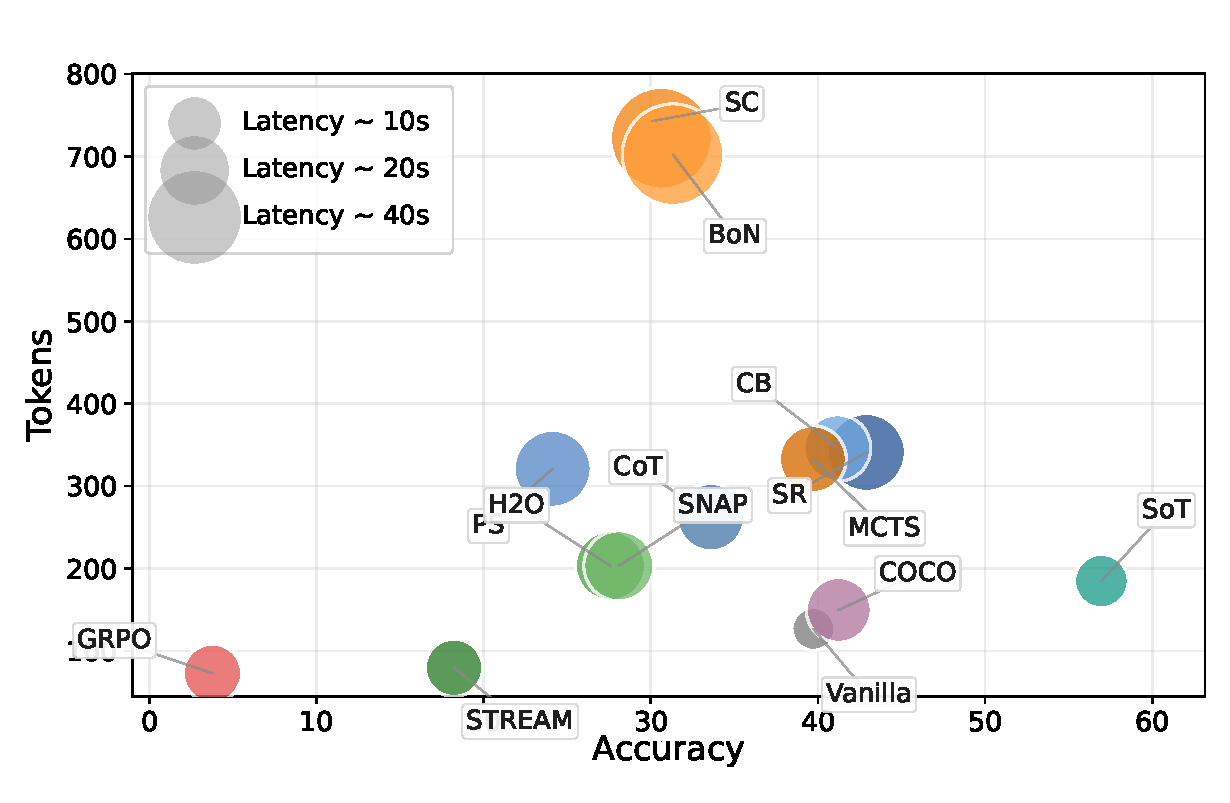
\includegraphics[width=1.0\textwidth]{figs/tradeoff_llama_ungrouped_baselines.pdf}
    \caption{Llama-3.1-8B}
\end{subfigure}
\hfill
\begin{subfigure}{0.49\textwidth}
    \centering
    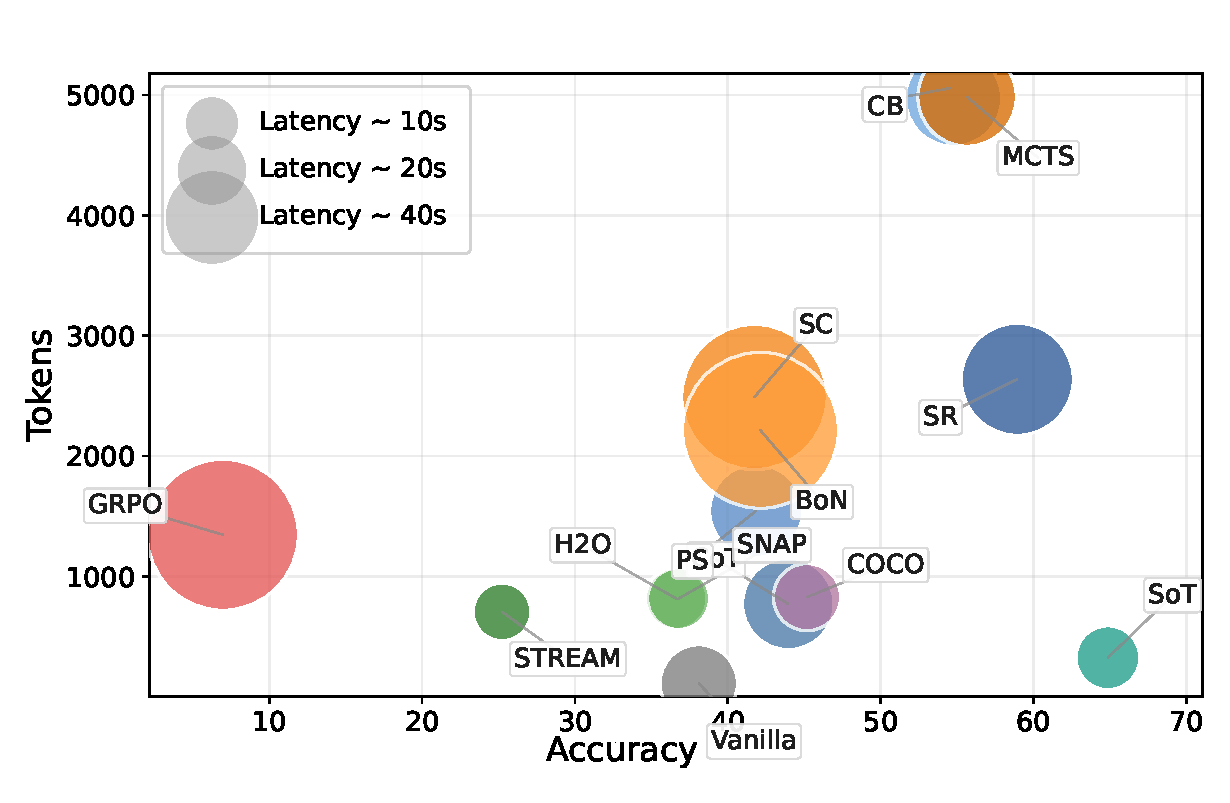
\includegraphics[width=1.0\textwidth]{figs/tradeoff_qwen14b_ungrouped_baselines.pdf}
    \caption{Qwen2.5-14B}
\end{subfigure}

\begin{subfigure}{0.49\textwidth}
    \centering
    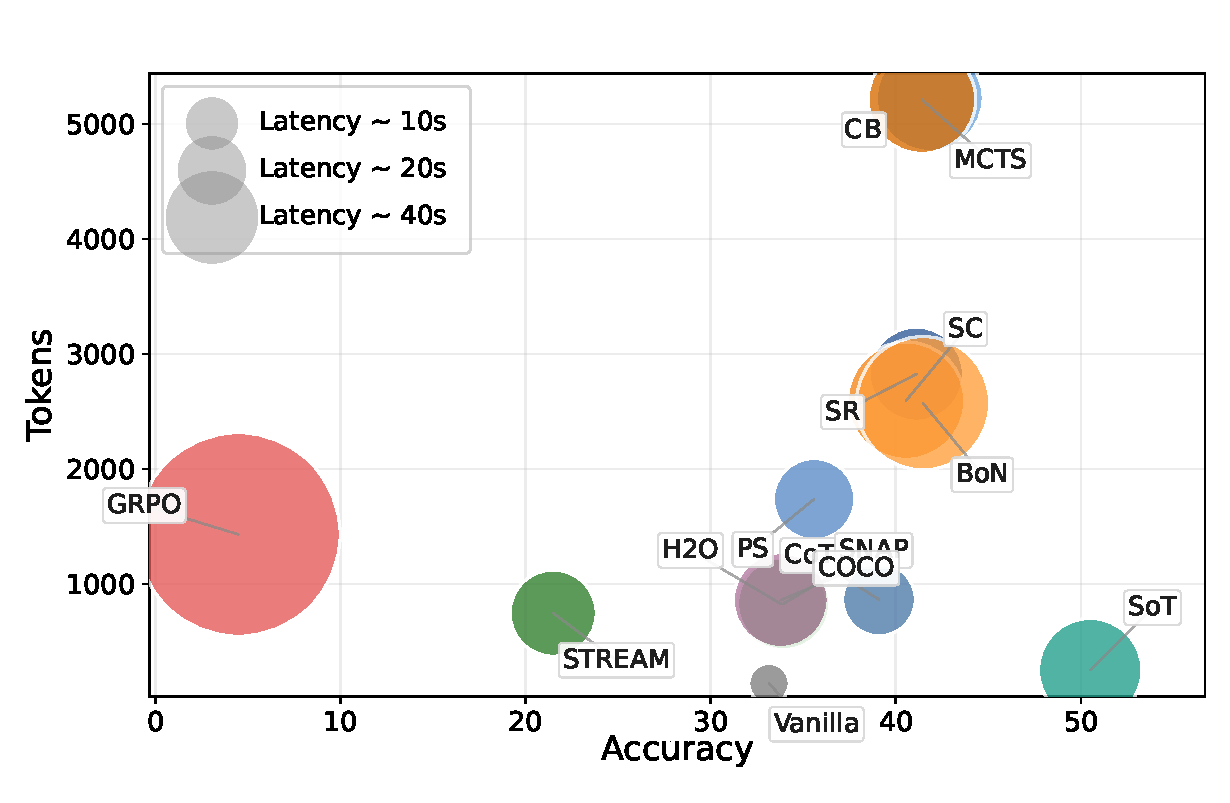
\includegraphics[width=1.0\textwidth]{figs/tradeoff_mixtral_ungrouped_baselines.pdf}
    \caption{Mixtral-8x7B}
\end{subfigure}
\hfill
\begin{subfigure}{0.49\textwidth}
    \centering
    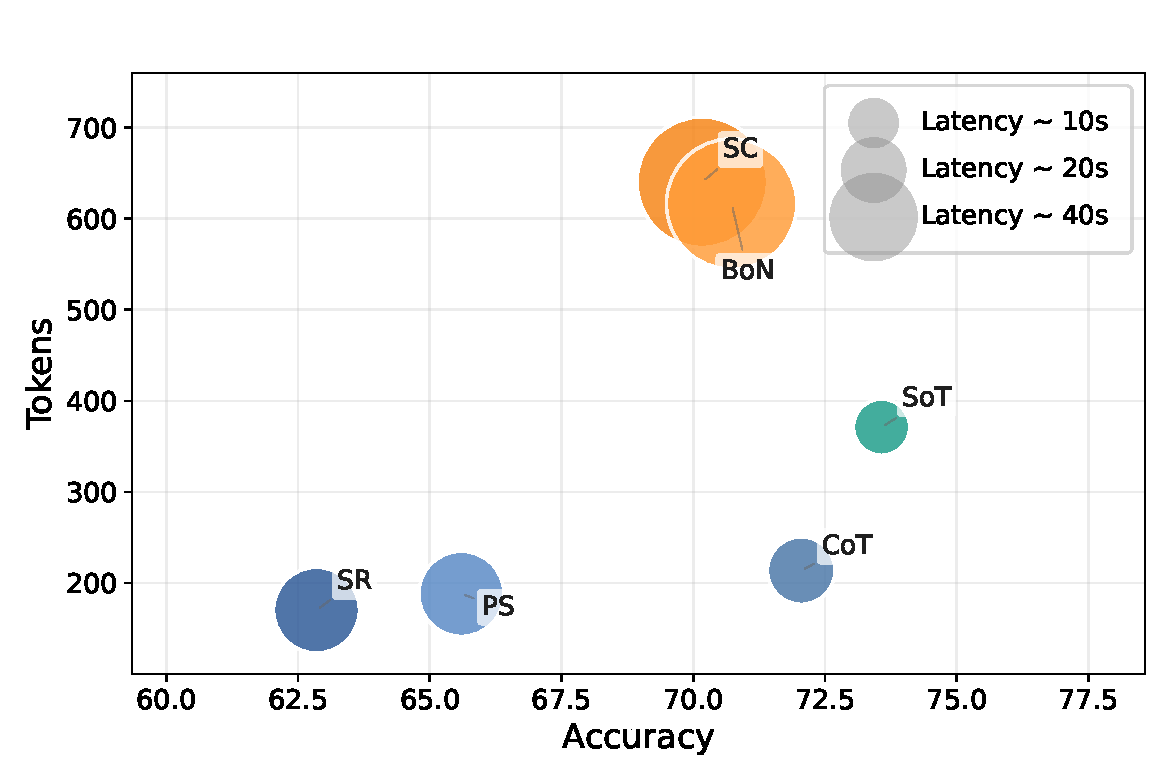
\includegraphics[width=1.0\textwidth]{figs/tradeoff_qwen3vl_ungrouped_baselines.pdf}
    \caption{Qwen3-VL-8B}
\end{subfigure}
\caption{\textbf{Extended accuracy--efficiency trade-off plots across backbones.} }
\label{fig:app_tradeoff_all}
\vspace{-3mm}
\end{figure*}

Figure~\ref{fig:app_tradeoff_all} shows a consistent cross-backbone pattern: methods that gain accuracy mainly through broader sampling/search move upward to high-token and high-latency regions, while SoT stays on or near the Pareto frontier.
On text backbones, SoT combines top-tier accuracy with substantially lower compute than search-heavy alternatives, indicating that its gains come from better control allocation rather than budget expansion.
The same trend also appears in multimodal transfer, supporting the view that state-conditioned evidence organization is a mechanism-level efficiency advantage rather than a backbone-specific tuning effect.

\begin{table*}[!t]
\centering
\caption{\textbf{Additional ablation results on Qwen2.5-14B.}}
\label{tab:app_ablation_qwen}
\footnotesize
\setlength{\tabcolsep}{1.75pt}%
\setlength{\aboverulesep}{0pt}%
\setlength{\belowrulesep}{0pt}%
\setlength{\extrarowheight}{0.75pt}%
\renewcommand{\arraystretch}{1.0}%
\begin{tabular}{l%
        @{\kern0.42em}!{\vrule width 0.4pt}@{\kern0.42em}%
        ccc%
        !{\vrule width 1pt}%
        ccc%
        !{\vrule width 1pt}%
        ccc%
        !{\vrule width 1pt}%
        ccc}
\toprule
\multirow{2}{*}{\textbf{Variant}}
& \multicolumn{3}{>{\columncolor[HTML]{E3F2FD}[\tabcolsep][\tabcolsep]}c!{\vrule width 1pt}}{\textbf{QS}}
& \multicolumn{3}{>{\columncolor[HTML]{E3F2FD}[\tabcolsep][\tabcolsep]}c!{\vrule width 1pt}}{\textbf{S\&C}}
& \multicolumn{3}{>{\columncolor[HTML]{E3F2FD}[\tabcolsep][\tabcolsep]}c!{\vrule width 1pt}}{\textbf{GU}}
& \multicolumn{3}{>{\columncolor[HTML]{E3F2FD}[\tabcolsep][\tabcolsep]}c}{\textbf{LCR}} \\
\cmidrule(lr){2-4} \cmidrule(lr){5-7} \cmidrule(lr){8-10} \cmidrule(lr){11-13}
& \textbf{acc.} & \textbf{tok.} & \textbf{lat.}
& \textbf{acc.} & \textbf{tok.} & \textbf{lat.}
& \textbf{acc.} & \textbf{tok.} & \textbf{lat.}
& \textbf{acc.} & \textbf{tok.} & \textbf{lat.} \\
\midrule
Full SoT & 66.1 & 545.8 & 16.8 & 76.8 & 408.4 & 19.0 & 81.3 & 133.2 & 5.8 & 25.2 & 254.0 & 23.4 \\
+ Threshold Tuning & 66.1 & 545.8 & 16.8 & 76.8 & 408.4 & 19.0 & 81.3 & 133.2 & 5.8 & 25.2 & 254.0 & 23.4 \\
\midrule
w/o Evid. Org. \(\mathcal{S}\) & 30.0 & \cellcolor[HTML]{EAECEF}{532.1} & 21.5 & 28.4 & 556.1 & 21.7 & 72.4 & 234.7 & 9.4 & \cellcolor[HTML]{EAECEF}{26.5} & 489.4 & \cellcolor[HTML]{EAECEF}{14.3} \\
w/o Stopping \(\mathcal{T}\) & \cellcolor[HTML]{EAECEF}{76.0} & 1401.9 & 37.4 & 32.4 & 2326.2 & 59.6 & 70.2 & 4175.0 & 100.9 & \cellcolor[HTML]{EAECEF}{31.7} & 2815.8 & 72.8 \\
w/o Geometry \(\delta_t\) & 56.5 & \cellcolor[HTML]{EAECEF}{77.9} & \cellcolor[HTML]{EAECEF}{3.9} & 23.1 & \cellcolor[HTML]{EAECEF}{45.8} & \cellcolor[HTML]{EAECEF}{2.5} & 73.0 & \cellcolor[HTML]{EAECEF}{25.4} & \cellcolor[HTML]{EAECEF}{0.9} & 21.2 & \cellcolor[HTML]{EAECEF}{48.2} & \cellcolor[HTML]{EAECEF}{2.2} \\
w/o Dynamics \((v_t,c_t)\) & \cellcolor[HTML]{EAECEF}{70.0} & 1220.9 & 32.1 & 30.8 & 910.0 & 26.9 & 70.6 & 1170.5 & 31.8 & \cellcolor[HTML]{EAECEF}{31.2} & 869.0 & 27.8 \\
w/o Uncertainty \(H_t\) & 62.5 & \cellcolor[HTML]{EAECEF}{306.0} & \cellcolor[HTML]{EAECEF}{7.6} & 30.6 & \cellcolor[HTML]{EAECEF}{255.6} & \cellcolor[HTML]{EAECEF}{7.6} & 73.0 & \cellcolor[HTML]{EAECEF}{61.3} & \cellcolor[HTML]{EAECEF}{1.9} & \cellcolor[HTML]{EAECEF}{33.6} & \cellcolor[HTML]{EAECEF}{190.2} & \cellcolor[HTML]{EAECEF}{6.6} \\
w/o Sent.-level Units & 62.5 & \cellcolor[HTML]{EAECEF}{306.0} & \cellcolor[HTML]{EAECEF}{7.6} & 30.6 & \cellcolor[HTML]{EAECEF}{255.6} & \cellcolor[HTML]{EAECEF}{7.6} & 73.0 & \cellcolor[HTML]{EAECEF}{61.3} & \cellcolor[HTML]{EAECEF}{1.9} & \cellcolor[HTML]{EAECEF}{33.6} & \cellcolor[HTML]{EAECEF}{190.2} & \cellcolor[HTML]{EAECEF}{6.6} \\
\bottomrule
\end{tabular}
\vspace{-5mm}
\end{table*}

\vspace{-2mm}
\subsection{Additional ablation results}
\label{app:additional_ablation}
\vspace{-1mm}

To test whether the main ablation pattern is specific to Llama-3.1-8B or reflects a more stable mechanism, we report additional ablations on Qwen2.5-14B, Mixtral-8$\times$7B, and Qwen3-VL-8B in Tables~\ref{tab:app_ablation_qwen}, \ref{tab:app_ablation_mixtral}, and \ref{tab:app_ablation_vlm}.
The cross-backbone pattern is consistent with the main-text ablation conclusion: removing evidence organization (\(\mathcal{S}\)) causes clear accuracy degradation (e.g., Qwen QS \(66.1\!\rightarrow\!30.0\), S\&C \(76.8\!\rightarrow\!28.4\); Mixtral QS \(46.3\!\rightarrow\!31.3\), LCR \(23.5\!\rightarrow\!3.0\)).
Removing stopping (\(\mathcal{T}\)) can occasionally increase one domain score, but it breaks efficiency by orders of magnitude (e.g., Qwen GU tokens \(133.2\!\rightarrow\!4175.0\); VLM Beans-M tokens \(493.5\!\rightarrow\!7511.4\), latency \(14.1\!\rightarrow\!206.5\)).
Meanwhile, threshold tuning is negligible on text backbones (identical to Full SoT on Qwen/Mixtral), and state-component removals typically trade short outputs for weaker accuracy, supporting the same mechanism-level claim as the main text: SoT gains come from the full closed-loop control, not from isolated calibration or trivial truncation.

\begin{table*}[t]
\centering
\caption{\textbf{Additional ablation results on Mixtral-8$\times$7B.}}
\label{tab:app_ablation_mixtral}
\footnotesize
\setlength{\tabcolsep}{1.75pt}%
\setlength{\aboverulesep}{0pt}%
\setlength{\belowrulesep}{0pt}%
\setlength{\extrarowheight}{0.75pt}%
\renewcommand{\arraystretch}{1.0}%
\begin{tabular}{l%
        @{\kern0.42em}!{\vrule width 0.4pt}@{\kern0.42em}%
        ccc%
        !{\vrule width 1pt}%
        ccc%
        !{\vrule width 1pt}%
        ccc%
        !{\vrule width 1pt}%
        ccc}
\toprule
\multirow{2}{*}{\textbf{Variant}}
& \multicolumn{3}{>{\columncolor[HTML]{E3F2FD}[\tabcolsep][\tabcolsep]}c!{\vrule width 1pt}}{\textbf{QS}}
& \multicolumn{3}{>{\columncolor[HTML]{E3F2FD}[\tabcolsep][\tabcolsep]}c!{\vrule width 1pt}}{\textbf{S\&C}}
& \multicolumn{3}{>{\columncolor[HTML]{E3F2FD}[\tabcolsep][\tabcolsep]}c!{\vrule width 1pt}}{\textbf{GU}}
& \multicolumn{3}{>{\columncolor[HTML]{E3F2FD}[\tabcolsep][\tabcolsep]}c}{\textbf{LCR}} \\
\cmidrule(lr){2-4} \cmidrule(lr){5-7} \cmidrule(lr){8-10} \cmidrule(lr){11-13}
& \textbf{acc.} & \textbf{tok.} & \textbf{lat.}
& \textbf{acc.} & \textbf{tok.} & \textbf{lat.}
& \textbf{acc.} & \textbf{tok.} & \textbf{lat.}
& \textbf{acc.} & \textbf{tok.} & \textbf{lat.} \\
\midrule
Full SoT & 46.3 & 248.2 & 43.8 & 51.7 & 329.8 & 62.6 & 72.5 & 143.6 & 28.0 & 23.5 & 260.6 & 62.8 \\
+ Threshold Tuning & 46.3 & 248.2 & 43.8 & 51.7 & 329.8 & 62.6 & 72.5 & 143.6 & 28.0 & 23.5 & 260.6 & 62.8 \\
\midrule
w/o Evid. Org. \(\mathcal{S}\) & 31.3 & 995.0 & 70.4 & 36.0 & 1002.6 & 65.8 & 63.2 & 836.8 & 51.0 & 3.0 & 921.1 & 90.7 \\
w/o Stopping \(\mathcal{T}\) & 31.3 & 995.0 & 64.0 & 36.0 & 1002.6 & 65.4 & 63.2 & 836.8 & 50.7 & 3.0 & 921.1 & 90.6 \\
w/o Geometry \(\delta_t\) & 34.0 & \cellcolor[HTML]{EAECEF}{58.1} & \cellcolor[HTML]{EAECEF}{11.8} & 30.7 & \cellcolor[HTML]{EAECEF}{56.9} & \cellcolor[HTML]{EAECEF}{13.3} & 57.6 & \cellcolor[HTML]{EAECEF}{50.8} & \cellcolor[HTML]{EAECEF}{7.6} & 3.3 & \cellcolor[HTML]{EAECEF}{54.0} & \cellcolor[HTML]{EAECEF}{13.8} \\
w/o Dynamics \((v_t,c_t)\) & 31.3 & 995.0 & 64.0 & 36.0 & 1002.6 & 65.4 & 63.2 & 836.8 & 50.7 & 3.0 & 921.1 & 90.6 \\
w/o Uncertainty \(H_t\) & 31.3 & 995.0 & 64.0 & 36.0 & 1002.6 & 65.4 & 63.2 & 836.8 & 50.7 & 3.0 & 921.1 & 90.6 \\
w/o Sent.-level Units & 31.3 & 995.0 & 64.0 & 36.0 & 1002.6 & 65.4 & 63.2 & 836.8 & 50.7 & 3.0 & 921.1 & 90.6 \\
\bottomrule
\end{tabular}
\vspace{-2mm}
\end{table*}

\begin{table*}[t]
\centering
\caption{\textbf{Additional ablation results on Qwen3-VL-8B.}}
\label{tab:app_ablation_vlm}
\footnotesize
\setlength{\tabcolsep}{1.75pt}%
\setlength{\aboverulesep}{0pt}%
\setlength{\belowrulesep}{0pt}%
\setlength{\extrarowheight}{0.75pt}%
\renewcommand{\arraystretch}{1.0}%
\begin{tabular}{l%
        @{\kern0.42em}!{\vrule width 0.4pt}@{\kern0.42em}%
        ccc%
        !{\vrule width 1pt}%
        ccc%
        !{\vrule width 1pt}%
        ccc%
        !{\vrule width 1pt}%
        ccc}
\toprule
\multirow{2}{*}{\textbf{Variant}}
& \multicolumn{3}{>{\columncolor[HTML]{E3F2FD}[\tabcolsep][\tabcolsep]}c!{\vrule width 1pt}}{\textbf{Beans-M}}
& \multicolumn{3}{>{\columncolor[HTML]{E3F2FD}[\tabcolsep][\tabcolsep]}c!{\vrule width 1pt}}{\textbf{F-MNIST}}
& \multicolumn{3}{>{\columncolor[HTML]{E3F2FD}[\tabcolsep][\tabcolsep]}c!{\vrule width 1pt}}{\textbf{DocVQA}}
& \multicolumn{3}{>{\columncolor[HTML]{E3F2FD}[\tabcolsep][\tabcolsep]}c}{\textbf{InfoVQA}} \\
\cmidrule(lr){2-4} \cmidrule(lr){5-7} \cmidrule(lr){8-10} \cmidrule(lr){11-13}
& \textbf{acc.} & \textbf{tok.} & \textbf{lat.}
& \textbf{acc.} & \textbf{tok.} & \textbf{lat.}
& \textbf{acc.} & \textbf{tok.} & \textbf{lat.}
& \textbf{acc.} & \textbf{tok.} & \textbf{lat.} \\
\midrule
Full SoT & 82.8 & 493.5 & 14.1 & 72.8 & 462.9 & 12.5 & 71.8 & 226.8 & 12.2 & 66.9 & 301.4 & 17.1 \\
+ Threshold Tuning & 80.8 & 453.7 & 13.6 & 52.8 & 423.1 & 13.5 & 71.8 & 226.8 & 12.2 & 60.0 & 335.4 & 17.3 \\
\midrule
w/o Evid. Org. \(\mathcal{S}\) & \cellcolor[HTML]{EAECEF}{83.8} & \cellcolor[HTML]{EAECEF}{473.6} & \cellcolor[HTML]{EAECEF}{13.3} & 47.0 & \cellcolor[HTML]{EAECEF}{458.1} & \cellcolor[HTML]{EAECEF}{12.4} & \cellcolor[HTML]{EAECEF}{72.5} & \cellcolor[HTML]{EAECEF}{189.9} & \cellcolor[HTML]{EAECEF}{10.6} & 59.5 & \cellcolor[HTML]{EAECEF}{258.8} & \cellcolor[HTML]{EAECEF}{14.5} \\
w/o Stopping \(\mathcal{T}\) & 82.8 & 7511.4 & 206.5 & 53.5 & 7436.5 & 188.5 & 64.6 & 4125.3 & 163.1 & 49.5 & 4827.8 & 203.7 \\
w/o Geometry \(\delta_t\) & 81.0 & 493.5 & \cellcolor[HTML]{EAECEF}{12.7} & 52.5 & 462.9 & \cellcolor[HTML]{EAECEF}{11.7} & \cellcolor[HTML]{EAECEF}{72.1} & 226.9 & \cellcolor[HTML]{EAECEF}{11.4} & 60.0 & \cellcolor[HTML]{EAECEF}{299.8} & \cellcolor[HTML]{EAECEF}{15.7} \\
w/o Dynamics \((v_t,c_t)\) & \cellcolor[HTML]{EAECEF}{84.8} & \cellcolor[HTML]{EAECEF}{79.4} & \cellcolor[HTML]{EAECEF}{2.2} & 43.2 & \cellcolor[HTML]{EAECEF}{75.9} & \cellcolor[HTML]{EAECEF}{2.0} & \cellcolor[HTML]{EAECEF}{72.1} & \cellcolor[HTML]{EAECEF}{48.4} & \cellcolor[HTML]{EAECEF}{4.1} & 60.0 & \cellcolor[HTML]{EAECEF}{72.9} & \cellcolor[HTML]{EAECEF}{5.7} \\
w/o Sent.-level Units & 80.8 & 493.5 & \cellcolor[HTML]{EAECEF}{12.7} & 52.8 & 462.9 & \cellcolor[HTML]{EAECEF}{11.7} & 71.8 & 226.8 & \cellcolor[HTML]{EAECEF}{11.5} & 60.0 & 301.4 & \cellcolor[HTML]{EAECEF}{16.6} \\
\bottomrule
\end{tabular}
\vspace{-3mm}
\end{table*}

\subsection{Limited-access variants and SoT-Judge}

We further expand the exploratory results in Section~\ref{sec:explore} with Tables~\ref{tab:app_boundary_qwen} and \ref{tab:app_boundary_mixtral}.
On Qwen2.5-14B, Training-free SoT stays competitive in QS/S\&C while improving LCR (\(26.2\) vs.\ \(17.6\)); SoT-Embed lags Top-3 on those averages yet matches the Top-3 LCR mean (\(18.1\) vs.\ \(17.6\)), so sentence-embedding trajectory summaries partially recover state-conditioned gains without privileged internals.
On Mixtral-8x7B, both limited-access runs lift QS/S\&C above Top-3 averages but trail on GU; SoT-Embed tracks Top-3 LCR more closely (\(23.3\) vs.\ \(22.7\)) than Training-free (\(21.5\)).

\begin{table*}[!b]
\centering
\caption{\textbf{Boundary studies of SoT on Qwen2.5-14B (accuracy, \%).}}
\vspace{-2mm}
\label{tab:app_boundary_qwen}
\footnotesize
\setlength{\tabcolsep}{5pt}%
\renewcommand{\arraystretch}{1.05}%
\begingroup
\setlength{\aboverulesep}{0pt}%
\setlength{\belowrulesep}{0pt}%
\setlength{\extrarowheight}{0.95pt}%
\begin{tabular}{l!{\vrule width 0.4pt}*{4}{c}!{\vrule width 1pt}*{6}{c}}
\toprule
& \multicolumn{4}{>{\cellcolor[HTML]{E3F2FD}}c!{\vrule width 1pt}}{\textbf{Quantitative Reasoning}} & \multicolumn{6}{>{\cellcolor[HTML]{E3F2FD}}c}{\textbf{Symbolic and Code}} \\
\cmidrule(lr){2-5}\cmidrule(lr){6-11}
& GSM8K & MATH & DROP & avg. & FOLIO & PW & BBH-T & HE & MBPP & avg. \\
\midrule
Top-3 Baseline avg. & 93.6 & 73.5 & 22.6 & 63.2 & 62.1 & 24.9 & 88.7 & 65.0 & 63.5 & 60.8 \\
SoT-Training-free & 81.8 & 60.8 & 34.6 & 59.1 & 49.5 & 30.2 & 77.0 & 53.0 & 50.4 & 52.0 \\
SoT-Embedding & 82.6 & 58.3 & 32.7 & 57.9 & 51.2 & 59.5 & 71.0 & 48.8 & 49.6 & 56.0 \\
\midrule
\end{tabular}
\par\addvspace{0.35ex}%
\begin{tabular}{l!{\vrule width 0.4pt}*{6}{c}!{\vrule width 1pt}*{4}{c}}
& \multicolumn{6}{>{\cellcolor[HTML]{E3F2FD}}c!{\vrule width 1pt}}{\textbf{General Understanding}} & \multicolumn{4}{>{\cellcolor[HTML]{E3F2FD}}c}{\textbf{Long-Context Reasoning}} \\
\cmidrule(lr){2-7}\cmidrule(lr){8-11}
& CSQA & StrQA & BoolQ & MMLU & RACE & avg. & HQA & NarQA & LB & avg. \\
\midrule
Top-3 Baseline avg. & 72.4 & 46.9 & 84.0 & 44.0 & 39.1 & 57.3 & 19.7 & 4.7 & 28.5 & 17.6 \\
SoT-Training-free & 59.3 & 55.2 & 70.0 & 45.4 & 52.7 & 56.5 & 22.9 & 34.2 & 21.6 & 26.2 \\
SoT-Embedding & 57.0 & 43.0 & 64.8 & 42.8 & 48.7 & 51.3 & 15.3 & 20.8 & 18.2 & 18.1 \\
\bottomrule
\end{tabular}%
\endgroup
\vspace{-1mm}
\end{table*}

\begin{table*}[!b]
\centering
\caption{\textbf{Boundary studies of SoT on Mixtral-8x7B (accuracy, \%).}}
\vspace{-2mm}
\label{tab:app_boundary_mixtral}
\footnotesize
\setlength{\tabcolsep}{5pt}%
\renewcommand{\arraystretch}{1.05}%
\begingroup
\setlength{\aboverulesep}{0pt}%
\setlength{\belowrulesep}{0pt}%
\setlength{\extrarowheight}{0.95pt}%
\begin{tabular}{l!{\vrule width 0.4pt}*{4}{c}!{\vrule width 1pt}*{6}{c}}
\toprule
& \multicolumn{4}{>{\cellcolor[HTML]{E3F2FD}}c!{\vrule width 1pt}}{\textbf{Quantitative Reasoning}} & \multicolumn{6}{>{\cellcolor[HTML]{E3F2FD}}c}{\textbf{Symbolic and Code}} \\
\cmidrule(lr){2-5}\cmidrule(lr){6-11}
& GSM8K & MATH & DROP & avg. & FOLIO & PW & BBH-T & HE & MBPP & avg. \\
\midrule
Top-3 Baseline avg. & 68.0 & 44.1 & 10.2 & 40.8 & 42.7 & 57.4 & 56.7 & 21.7 & 40.4 & 43.8 \\
SoT-Training-free & 75.2 & 52.2 & 32.3 & 53.2 & 31.3 & 50.5 & 63.0 & 56.1 & 49.2 & 50.0 \\
SoT-Embedding & 76.0 & 52.0 & 34.3 & 54.1 & 30.8 & 50.5 & 63.0 & 55.5 & 49.2 & 49.8 \\
\midrule
\end{tabular}
\par\addvspace{0.35ex}%
\begin{tabular}{l!{\vrule width 0.4pt}*{6}{c}!{\vrule width 1pt}*{4}{c}}
& \multicolumn{6}{>{\cellcolor[HTML]{E3F2FD}}c!{\vrule width 1pt}}{\textbf{General Understanding}} & \multicolumn{4}{>{\cellcolor[HTML]{E3F2FD}}c}{\textbf{Long-Context Reasoning}} \\
\cmidrule(lr){2-7}\cmidrule(lr){8-11}
& CSQA & StrQA & BoolQ & MMLU & RACE & avg. & HQA & NarQA & LB & avg. \\
\midrule
Top-3 Baseline avg. & 64.2 & 66.6 & 81.1 & 58.9 & 55.7 & 65.3 & 15.0 & 15.8 & 37.4 & 22.7 \\
SoT-Training-free & 49.5 & 54.5 & 66.5 & 50.8 & 48.3 & 53.9 & 19.7 & 24.4 & 20.5 & 21.5 \\
SoT-Embedding & 49.3 & 44.3 & 52.5 & 51.2 & 47.5 & 49.0 & 20.3 & 24.0 & 25.5 & 23.3 \\
\bottomrule
\end{tabular}%
\endgroup
\vspace{-1mm}
\end{table*}

\clearpage{}
We report full judge behavior in Table~\ref{tab:app_judge_breakdown}.
The same insight as the main section is reinforced: SoT-Judge's largest gains concentrate in trajectory-structure-sensitive regimes (especially LCR, e.g., GPT-5.4 \(84.0\) vs.\ \(\le 12.3\) for baselines, Claude 4.7 \(95.7\) vs.\ \(\le 11.5\), Qwen-Max \(87.1\) vs.\ \(\le 11.1\)), while remaining competitive in GU/S\&C averages, suggesting that trajectory-state signals are most informative where long-horizon coherence, not local answer matching, is the primary bottleneck.

\begin{table*}[!t]
\centering
\caption{\textbf{Black-box judging with trajectory-based SoT (dataset breakdown, \%).}}
\label{tab:app_judge_breakdown}
\vspace{-2mm}
\footnotesize
\begingroup
\setlength{\tabcolsep}{2.65pt}%
\setlength{\aboverulesep}{0pt}%
\setlength{\belowrulesep}{0pt}%
\setlength{\extrarowheight}{0.88pt}%
\renewcommand{\arraystretch}{0.99}%

\begin{tabular}{ll!{\vrule width 0.4pt} ccc>{\columncolor[HTML]{EAECEF}}c!{\vrule width 1pt}ccccc>{\columncolor[HTML]{EAECEF}}c}
\toprule
\textbf{Model} & \textbf{Method}
& \multicolumn{4}{>{\cellcolor[HTML]{E3F2FD}}c!{\vrule width 1pt}}{\textbf{Quantitative Reasoning}}
& \multicolumn{6}{>{\cellcolor[HTML]{E3F2FD}}c}{\textbf{Symbolic and Code}} \\
\cmidrule(lr){3-6}\cmidrule(lr){7-12}
& & \textbf{GSM8K} & \textbf{MATH} & \textbf{DROP} & \textbf{avg.}
& \textbf{FOLIO} & \textbf{PW} & \textbf{BBH-T} & \textbf{HE} & \textbf{MBPP} & \textbf{avg.} \\
\midrule
\multirow{4}{*}{GPT-5.4}
& Self-Consistency & \underline{92.0} & 78.0 & 5.0 & 65.6 & 69.0 & 77.0 & \underline{86.0} & \underline{87.0} & 77.0 & \underline{77.8} \\
& Self-Verification & \underline{92.0} & 78.0 & 5.0 & 65.6 & 62.0 & 79.0 & 85.0 & \underline{87.0} & \underline{78.0} & 77.4 \\
& LLM-as-a-Judge & \underline{92.0} & \underline{79.0} & 4.0 & 65.7 & \underline{70.0} & 76.0 & \underline{86.0} & 86.0 & \underline{78.0} & 77.7 \\
& \textbf{SoT-Judge} & \textbf{91.0} & \underline{\textbf{79.0}} & \underline{\textbf{92.0}} & \underline{\textbf{87.2}} & \textbf{61.0} & \underline{\textbf{80.0}} & \textbf{82.0} & \textbf{86.0} & \underline{\textbf{78.0}} & \textbf{77.2} \\
\midrule
\multirow{4}{*}{Claude 4.7}
& Self-Consistency & 90.0 & 78.0 & 1.0 & 63.8 & 65.0 & 73.0 & \underline{58.0} & 94.0 & 86.0 & 76.2 \\
& Self-Verification & \underline{94.1} & \underline{80.0} & 4.0 & 66.9 & \underline{71.4} & \underline{80.0} & 57.1 & \underline{98.4} & \underline{94.4} & \underline{82.3} \\
& LLM-as-a-Judge & 90.0 & 78.0 & 2.0 & 64.0 & 66.0 & 74.0 & 57.0 & 94.0 & 86.0 & 76.6 \\
& \textbf{SoT-Judge} & \textbf{92.0} & \underline{\textbf{80.0}} & \underline{\textbf{96.0}} & \underline{\textbf{89.0}} & \textbf{58.0} & \textbf{78.0} & \textbf{54.0} & \textbf{97.0} & \textbf{87.0} & \textbf{77.0} \\
\midrule
\multirow{4}{*}{Qwen-Max}
& Self-Consistency & 88.0 & 82.8 & 3.0 & 65.0 & 76.0 & \underline{86.0} & \underline{81.0} & \underline{83.8} & 73.0 & \underline{80.5} \\
& Self-Verification & 46.7 & 35.3 & 6.0 & 32.7 & \underline{80.6} & 82.9 & 74.5 & 81.5 & 70.0 & 78.6 \\
& LLM-as-a-Judge & \underline{92.0} & 82.8 & 3.0 & 66.7 & 74.0 & \underline{86.0} & \underline{81.0} & \underline{83.8} & \underline{74.0} & 80.4 \\
& \textbf{SoT-Judge} & \textbf{84.0} & \underline{\textbf{93.1}} & \underline{\textbf{90.0}} & \underline{\textbf{88.5}} & \textbf{71.0} & \textbf{80.0} & \textbf{80.0} & \textbf{79.0} & \textbf{68.0} & \textbf{75.5} \\
\midrule
\end{tabular}
\par\addvspace{0.35ex}%
\begin{tabular}{ll!{\vrule width 0.4pt} ccccc>{\columncolor[HTML]{EAECEF}}c!{\vrule width 1pt}ccc>{\columncolor[HTML]{EAECEF}}c}
\textbf{Model} & \textbf{Method}
& \multicolumn{6}{>{\cellcolor[HTML]{E3F2FD}}c!{\vrule width 1pt}}{\textbf{General Understanding}}
& \multicolumn{4}{>{\cellcolor[HTML]{E3F2FD}}c}{\textbf{Long-Context Reasoning}} \\
\cmidrule(lr){3-8}\cmidrule(lr){9-12}
& & \textbf{CSQA} & \textbf{StrQA} & \textbf{BoolQ} & \textbf{MMLU} & \textbf{RACE} & \textbf{avg.}
& \textbf{HQA} & \textbf{NarQA} & \textbf{LB} & \textbf{avg.} \\
\midrule
\multirow{4}{*}{GPT-5.4}
& Self-Consistency & 85.0 & 82.0 & \underline{94.0} & 76.0 & 70.0 & 81.7 & 7.0 & 9.0 & 34.0 & 12.3 \\
& Self-Verification & 84.0 & 81.0 & 93.0 & 75.0 & 70.0 & 80.8 & 7.0 & 9.0 & 32.0 & 11.9 \\
& LLM-as-a-Judge & \underline{86.0} & \underline{85.0} & \underline{94.0} & 75.0 & 70.0 & \underline{82.2} & 7.0 & 9.0 & 33.0 & 12.1 \\
& \textbf{SoT-Judge} & \textbf{85.0} & \textbf{82.0} & \textbf{84.0} & \underline{\textbf{77.0}} & \underline{\textbf{73.0}} & \textbf{80.4} & \underline{\textbf{90.0}} & \underline{\textbf{87.0}} & \underline{\textbf{61.0}} & \underline{\textbf{84.0}} \\
\midrule
\multirow{4}{*}{Claude 4.7}
& Self-Consistency & \underline{83.0} & 86.0 & \underline{95.0} & 76.0 & 78.0 & \underline{83.5} & 11.0 & 1.0 & 3.0 & 5.9 \\
& Self-Verification & 46.5 & 87.2 & 94.0 & 23.3 & 62.7 & 60.8 & 23.0 & 1.0 & 4.0 & 11.5 \\
& LLM-as-a-Judge & 82.0 & 85.0 & \underline{95.0} & \underline{77.0} & \underline{79.0} & \underline{83.5} & 11.0 & 1.0 & 4.0 & 6.0 \\
& \textbf{SoT-Judge} & \textbf{81.0} & \underline{\textbf{88.0}} & \textbf{85.0} & \textbf{80.0} & \underline{\textbf{79.0}} & \textbf{82.7} & \underline{\textbf{93.0}} & \underline{\textbf{98.0}} & \underline{\textbf{98.0}} & \underline{\textbf{95.7}} \\
\midrule
\multirow{4}{*}{Qwen-Max}
& Self-Consistency & 82.0 & 82.0 & 91.0 & 77.0 & \underline{88.0} & 83.5 & 11.0 & 1.0 & 31.5 & 10.6 \\
& Self-Verification & \underline{86.7} & \underline{86.2} & \underline{93.8} & \underline{80.6} & 85.0 & \underline{86.2} & 1.9 & 1.4 & 31.5 & 6.6 \\
& LLM-as-a-Judge & 84.0 & 82.0 & 93.0 & 77.0 & \underline{88.0} & 84.2 & 12.0 & 1.0 & 31.5 & 11.1 \\
& \textbf{SoT-Judge} & \textbf{84.0} & \textbf{84.0} & \textbf{91.0} & \textbf{80.0} & \textbf{87.0} & \textbf{84.8} & \underline{\textbf{94.0}} & \underline{\textbf{89.0}} & \underline{\textbf{64.0}} & \underline{\textbf{87.1}} \\
\bottomrule
\end{tabular}%
\endgroup
\vspace{-2mm}
\end{table*}

\subsection{Sensitivity to trajectory quality}
\label{app:traj_quality}
We test whether SoT remains informative when the offline trajectory pool is collected or curated differently, with Llama-3.1-8B results in Table~\ref{tab:app_traj_quality} (default HQ pool vs.\ weaker variants and training-free SoT).
The table shows a consistent split: weaker pools largely leave QS/S\&C accuracy near plateau but disproportionately hurt GU/LCR while greatly inflating tokens and latency relative to HQ; training-free SoT sits in the same heavy-trajectory regime with domain-mixed accuracy shifts.
Overall, curation affects whether supervision yields a cheap, reliable trajectory-level control signal more than it acts as a uniform rescaling of backbone capability.

\begin{table*}[!b]
\centering
\caption{\textbf{Sensitivity to trajectory-pool quality on Llama-3.1-8B}.}
\label{tab:app_traj_quality}
\vspace{-2mm}
\footnotesize
\begingroup
\setlength{\tabcolsep}{4.2pt}%
\setlength{\aboverulesep}{0pt}%
\setlength{\belowrulesep}{0pt}%
\setlength{\extrarowheight}{0.75pt}%
\renewcommand{\arraystretch}{1.0}%
\begin{tabular}{l!{\vrule width 0.4pt}ccc!{\vrule width 1pt}ccc!{\vrule width 1pt}ccc!{\vrule width 1pt}ccc}
\toprule
\multirow{2}{*}{\textbf{Trajectory pool}} 
& \multicolumn{3}{>{\cellcolor[HTML]{E3F2FD}}c!{\vrule width 1pt}}{\textbf{QS}} 
& \multicolumn{3}{>{\cellcolor[HTML]{E3F2FD}}c!{\vrule width 1pt}}{\textbf{S\&C}} 
& \multicolumn{3}{>{\cellcolor[HTML]{E3F2FD}}c!{\vrule width 1pt}}{\textbf{GU}} 
& \multicolumn{3}{>{\cellcolor[HTML]{E3F2FD}}c}{\textbf{LCR}} \\
\cmidrule(lr){2-4} \cmidrule(lr){5-7} \cmidrule(lr){8-10} \cmidrule(lr){11-13}
& \textbf{acc.} & \textbf{tok.} & \textbf{lat.}
& \textbf{acc.} & \textbf{tok.} & \textbf{lat.}
& \textbf{acc.} & \textbf{tok.} & \textbf{lat.}
& \textbf{acc.} & \textbf{tok.} & \textbf{lat.} \\
\midrule
Full HQ pool & 70.8 & 247.9 & 6.3 & 57.1 & 324.2 & 11.1 & 75.5 & 58.0 & 1.6 & 37.3 & 121.1 & 97.5 \\
No filter & 71.3 & 931.3 & 30.0 & 57.7 & 1080.8 & 84.1 & 49.2 & 886.0 & 29.5 & 21.5 & 900.9 & 91.5 \\
Weak filter & 71.3 & 931.3 & 24.3 & 57.7 & 1080.8 & 34.5 & 49.2 & 886.0 & 17.7 & 21.3 & 900.9 & 90.7 \\
No pipeline & 71.3 & 931.3 & 26.1 & 57.7 & 1080.8 & 53.4 & 49.2 & 886.0 & 49.3 & 21.5 & 900.9 & 89.3 \\
Training-free & 72.3 & 917.4 & 26.0 & 58.3 & 1078.9 & 35.0 & 53.8 & 906.6 & 19.7 & 28.1 & 872.9 & 95.8 \\
\bottomrule
\end{tabular}%
\endgroup
\vspace{-2mm}
\end{table*}

\clearpage
\vspace{-3mm}
\section{Case Studies}
\label{app:case_studies}
\vspace{-2mm}

\subsection{Case 1: Quantitative Reasoning (QS)}
\vspace{-1mm}
Figure~\ref{fig:app_case_arithmetic} follows a staged numeric workflow (per-store accounting, then comparison).
Intermediate steps reuse only the quantities that remain algebraically active in the next operation, and \(p(\mathrm{stop})\) ramps once the competing subtotals are both fixed: the mechanism reads as \emph{derivation support} that is pruned as subgoals close, not as uniform context replay.
\vspace{-3mm}

\begin{figure}[H]
\centering
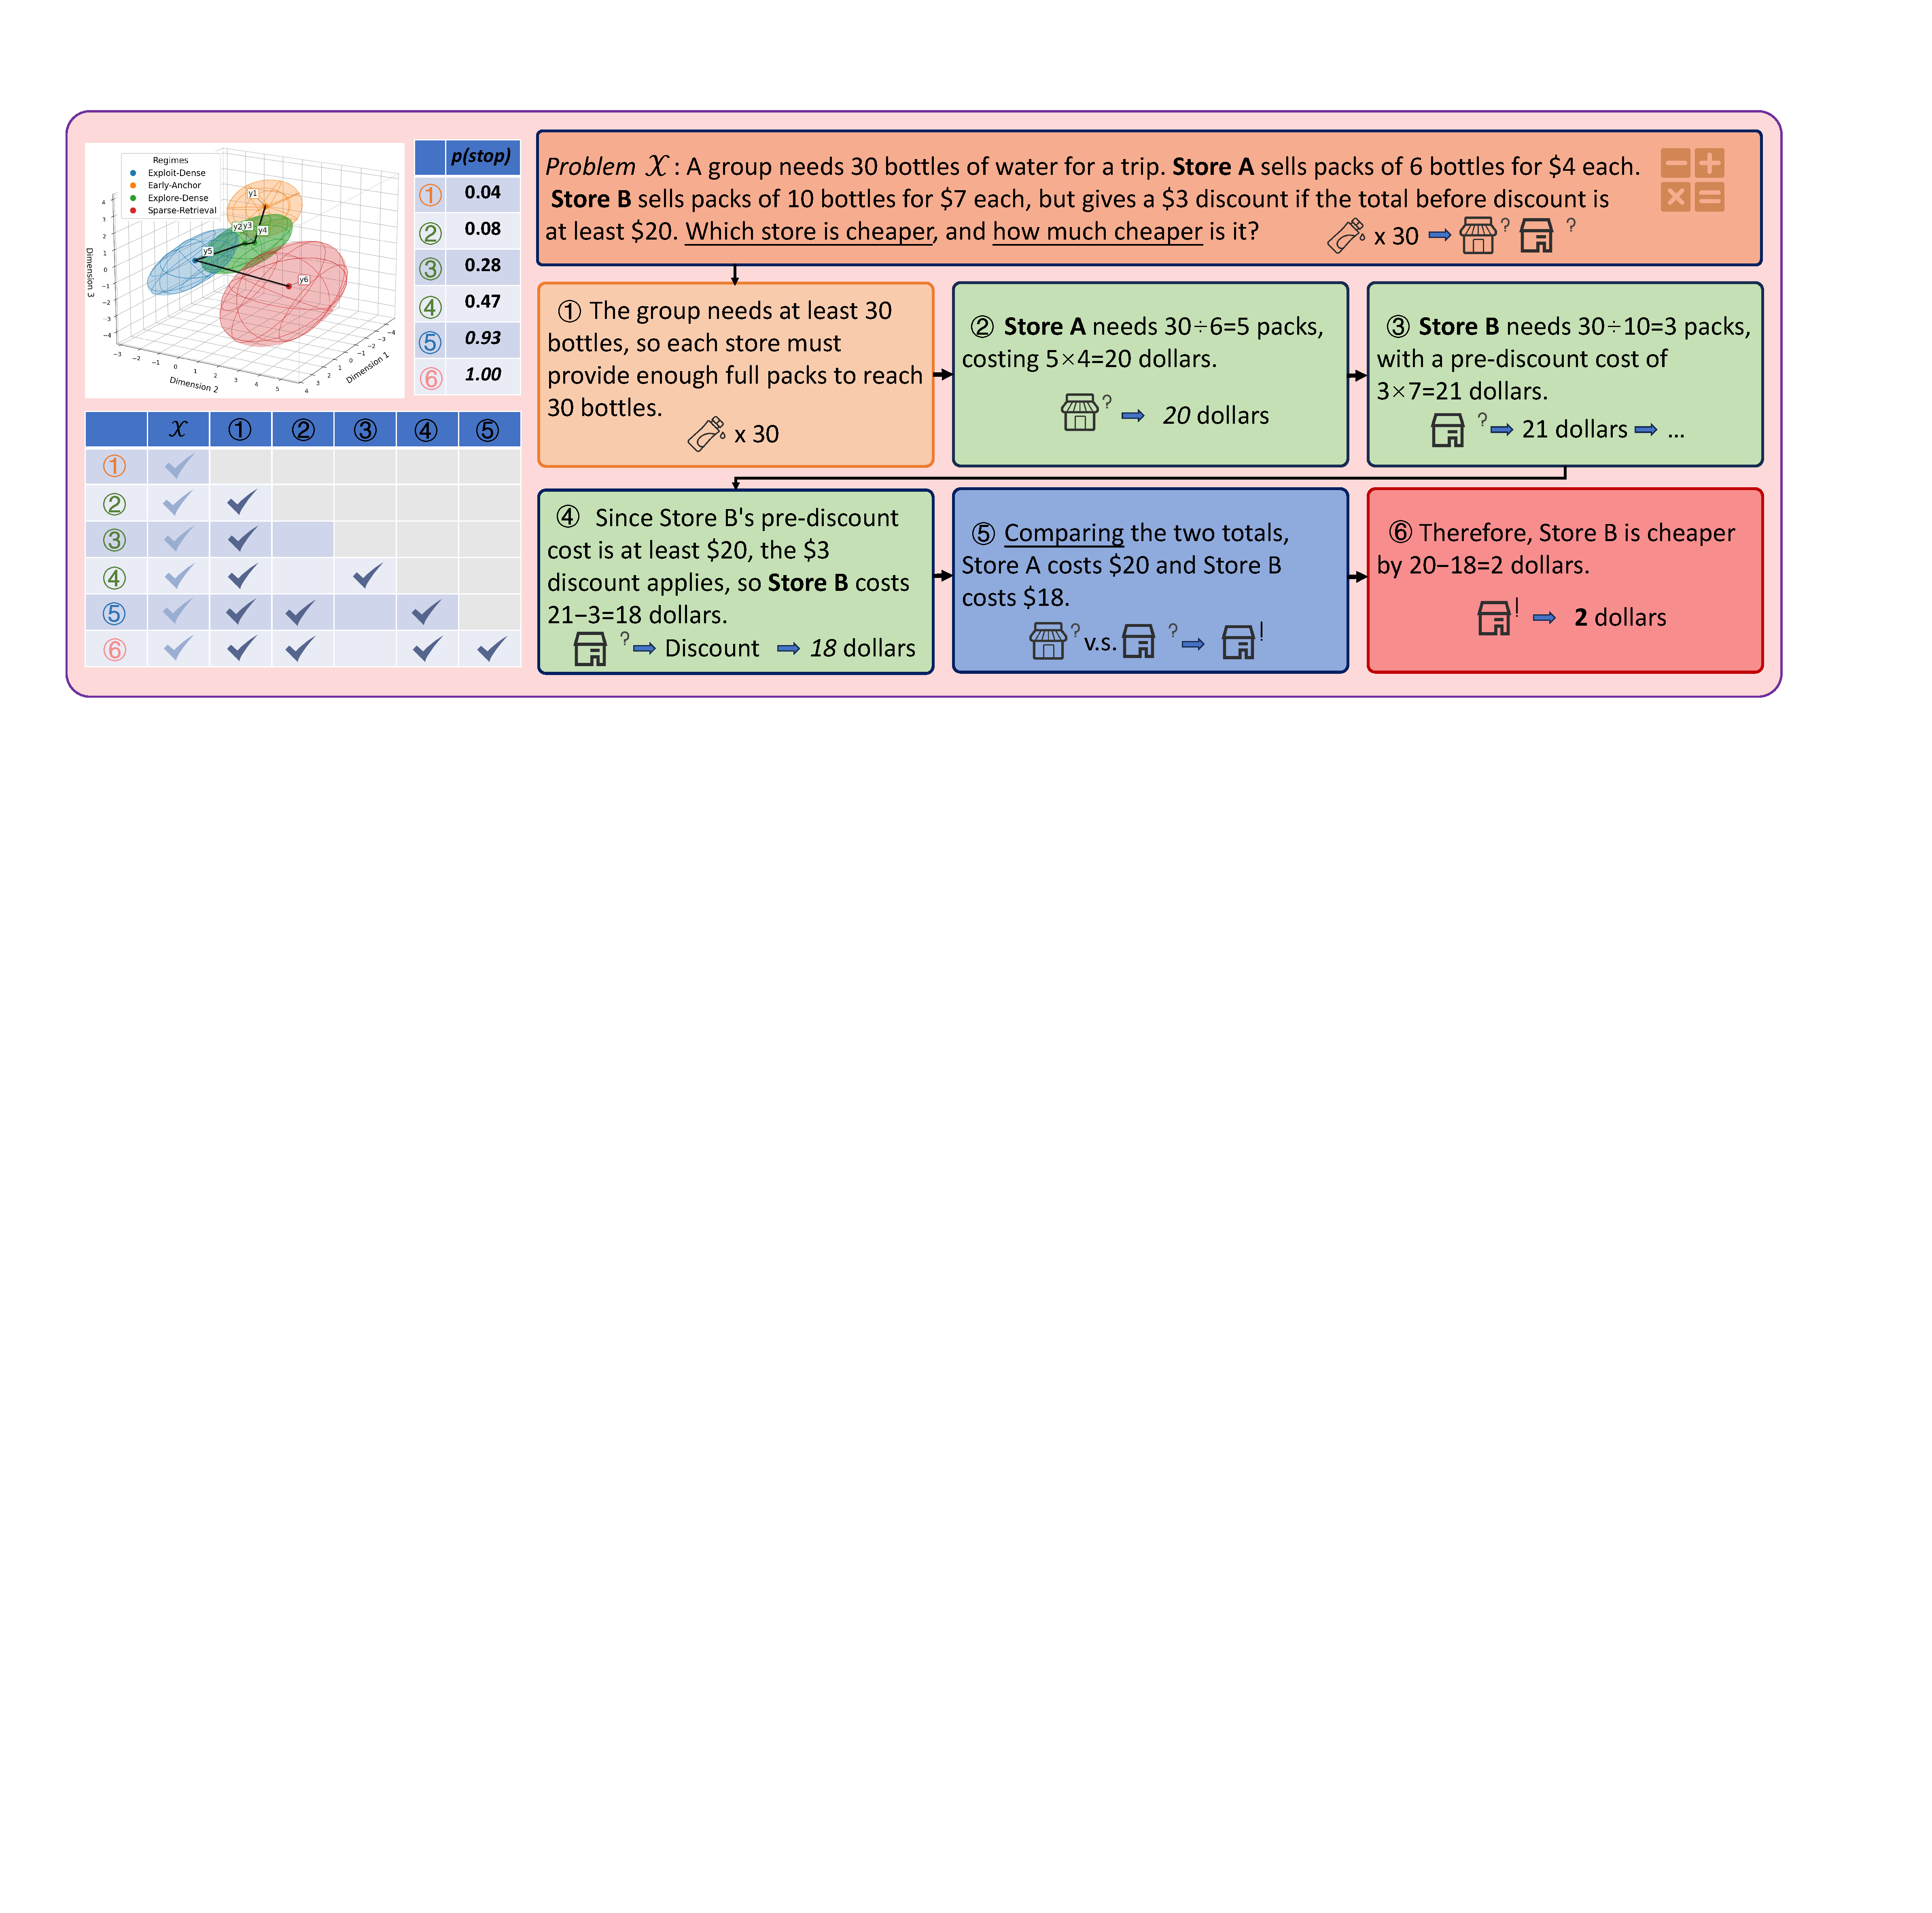
\includegraphics[width=0.97\textwidth]{figs/app_case_arithmetic.pdf}
\vspace{-2mm}
\caption{Case study on Quantitative Reasoning (QS).}
\label{fig:app_case_arithmetic}
\end{figure}

\subsection{Case 2: General Understanding (GU)}
\vspace{-1mm}
Figure~\ref{fig:app_case_cki} is a commonsense elimination problem: late steps depend on the prompt and the locally decisive intermediates while dropping earlier scaffolding—a pattern that matters when verbal distractors would otherwise pollute a full-history transcript.
\vspace{-3mm}

\begin{figure}[H]
\centering
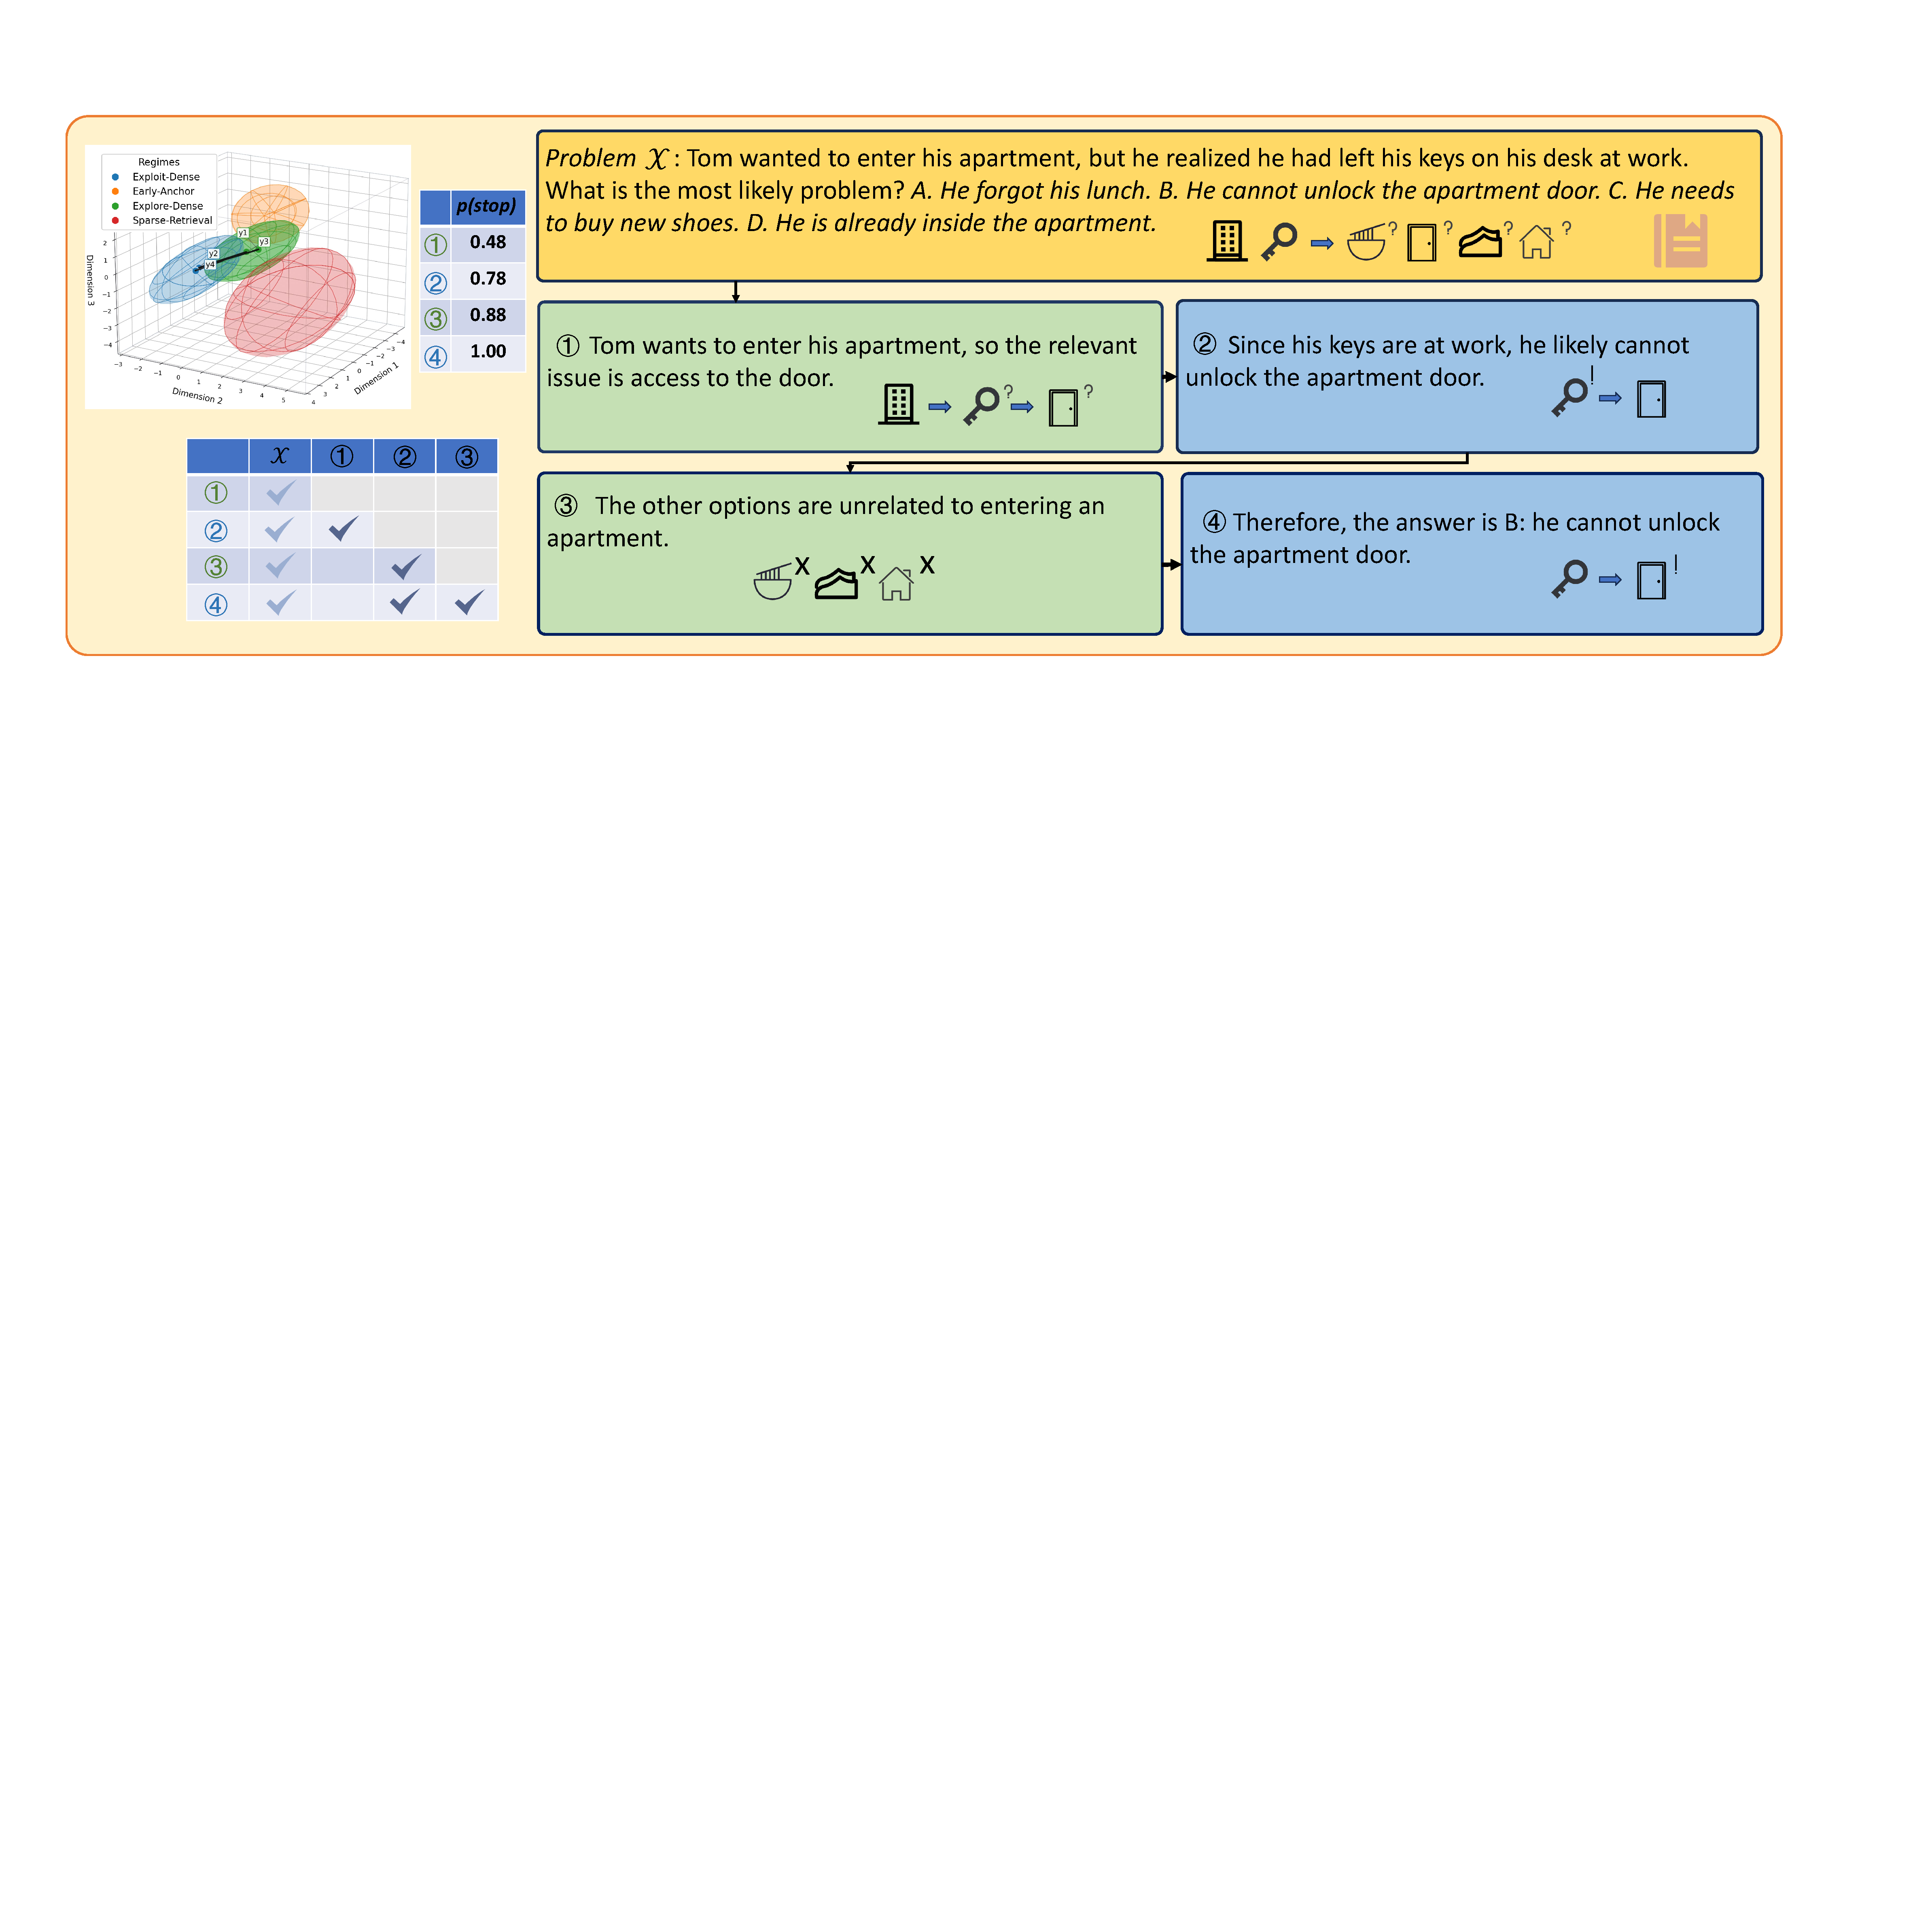
\includegraphics[width=0.97\textwidth]{figs/app_case_cki.pdf}
\vspace{-2mm}
\caption{Case study on General Understanding (GU).}
\label{fig:app_case_cki}
\end{figure}

\subsection{Case 3: Symbolic and Code (S\&C)}
\vspace{-1mm}
Figure~\ref{fig:app_case_formal} chains explicit rules forward but the evidence matrix is non-monotone—later steps re-anchor on conclusions and skip obsolete rule instantiations—so correctness is tied to \emph{structural} carry (what still entails the next judgment), not to preserving the full forward chain verbatim.
\vspace{-3mm}

\begin{figure}[H]
\centering
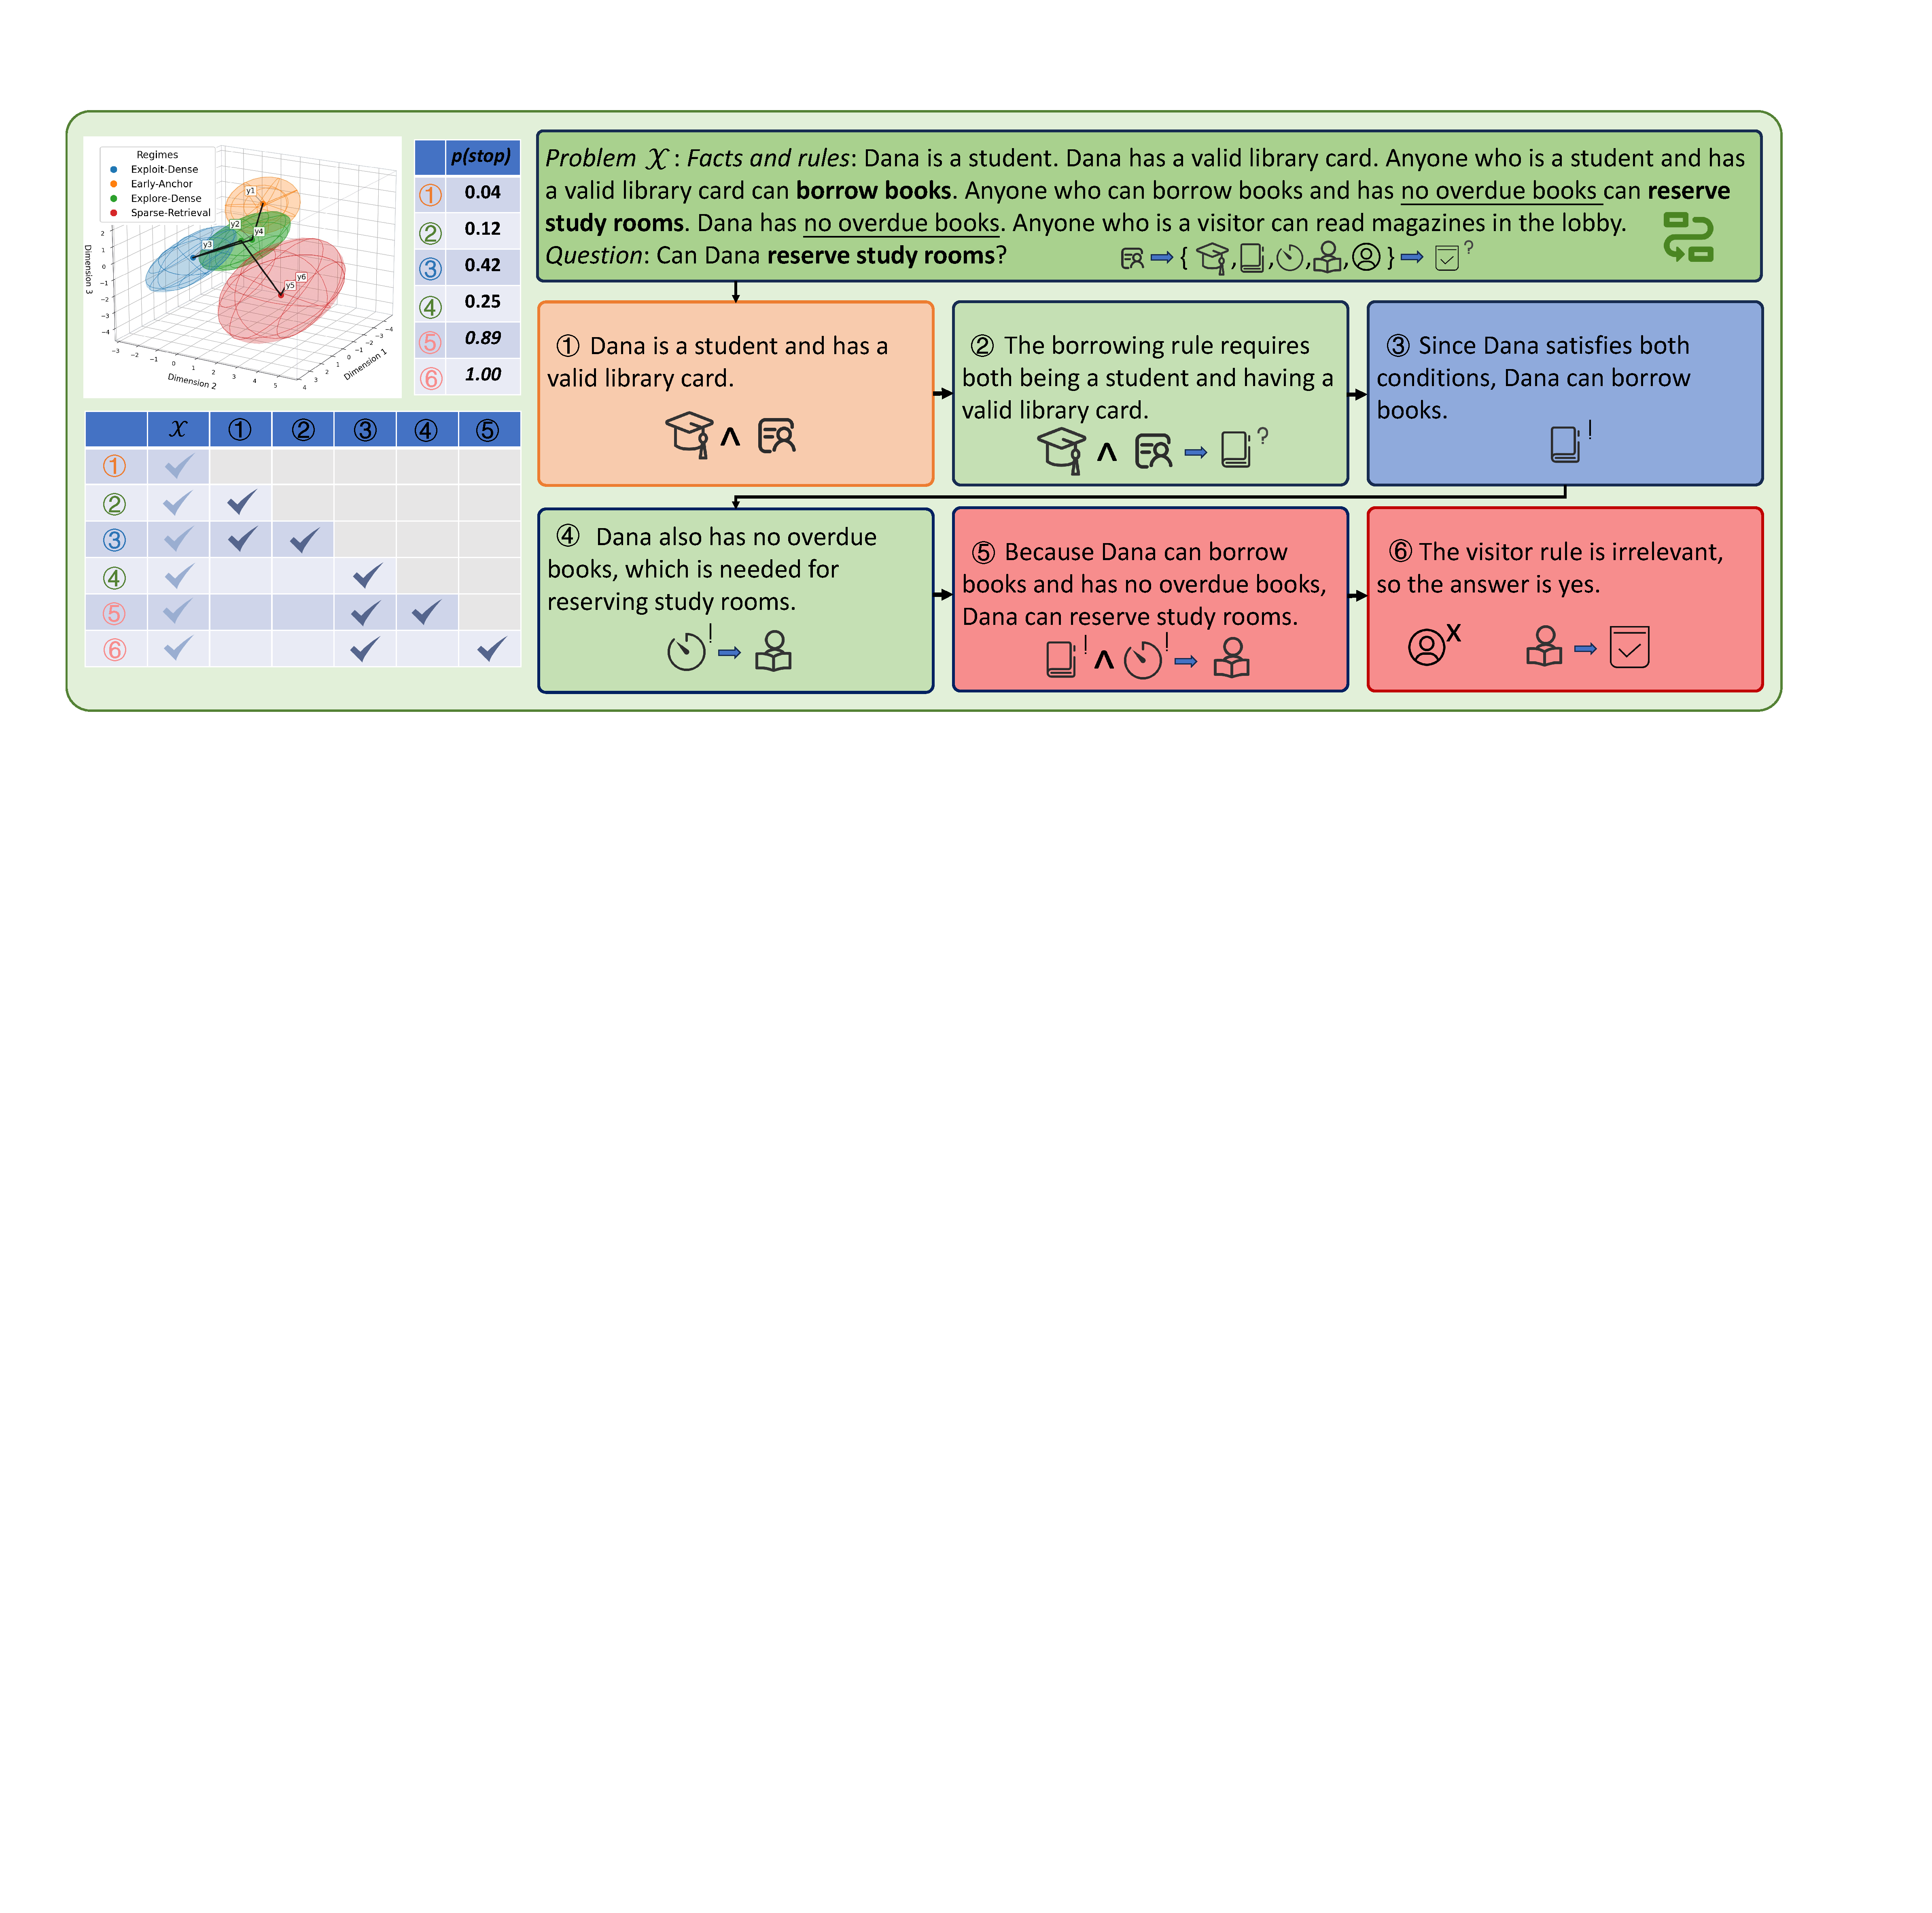
\includegraphics[width=0.97\textwidth]{figs/app_case_formal.pdf}
\vspace{-2mm}
\caption{Case study on Symbolic and Code (S\&C).}
\label{fig:app_case_formal}
\end{figure}

\subsection{Case 4: Long-Context Reasoning (LCR)}
\vspace{-1mm}
Figure~\ref{fig:app_case_longcontext} integrates constraints spread across a long narrative; the trajectory lingers in exploration-like regimes while facts are harvested, then compresses into a sparse-retrieval phase that fuses only the clauses still relevant to the contrastive \emph{why} question—i.e., compositional support rather than verbatim long-context carry.
\vspace{-3mm}

\begin{figure}[H]
\centering
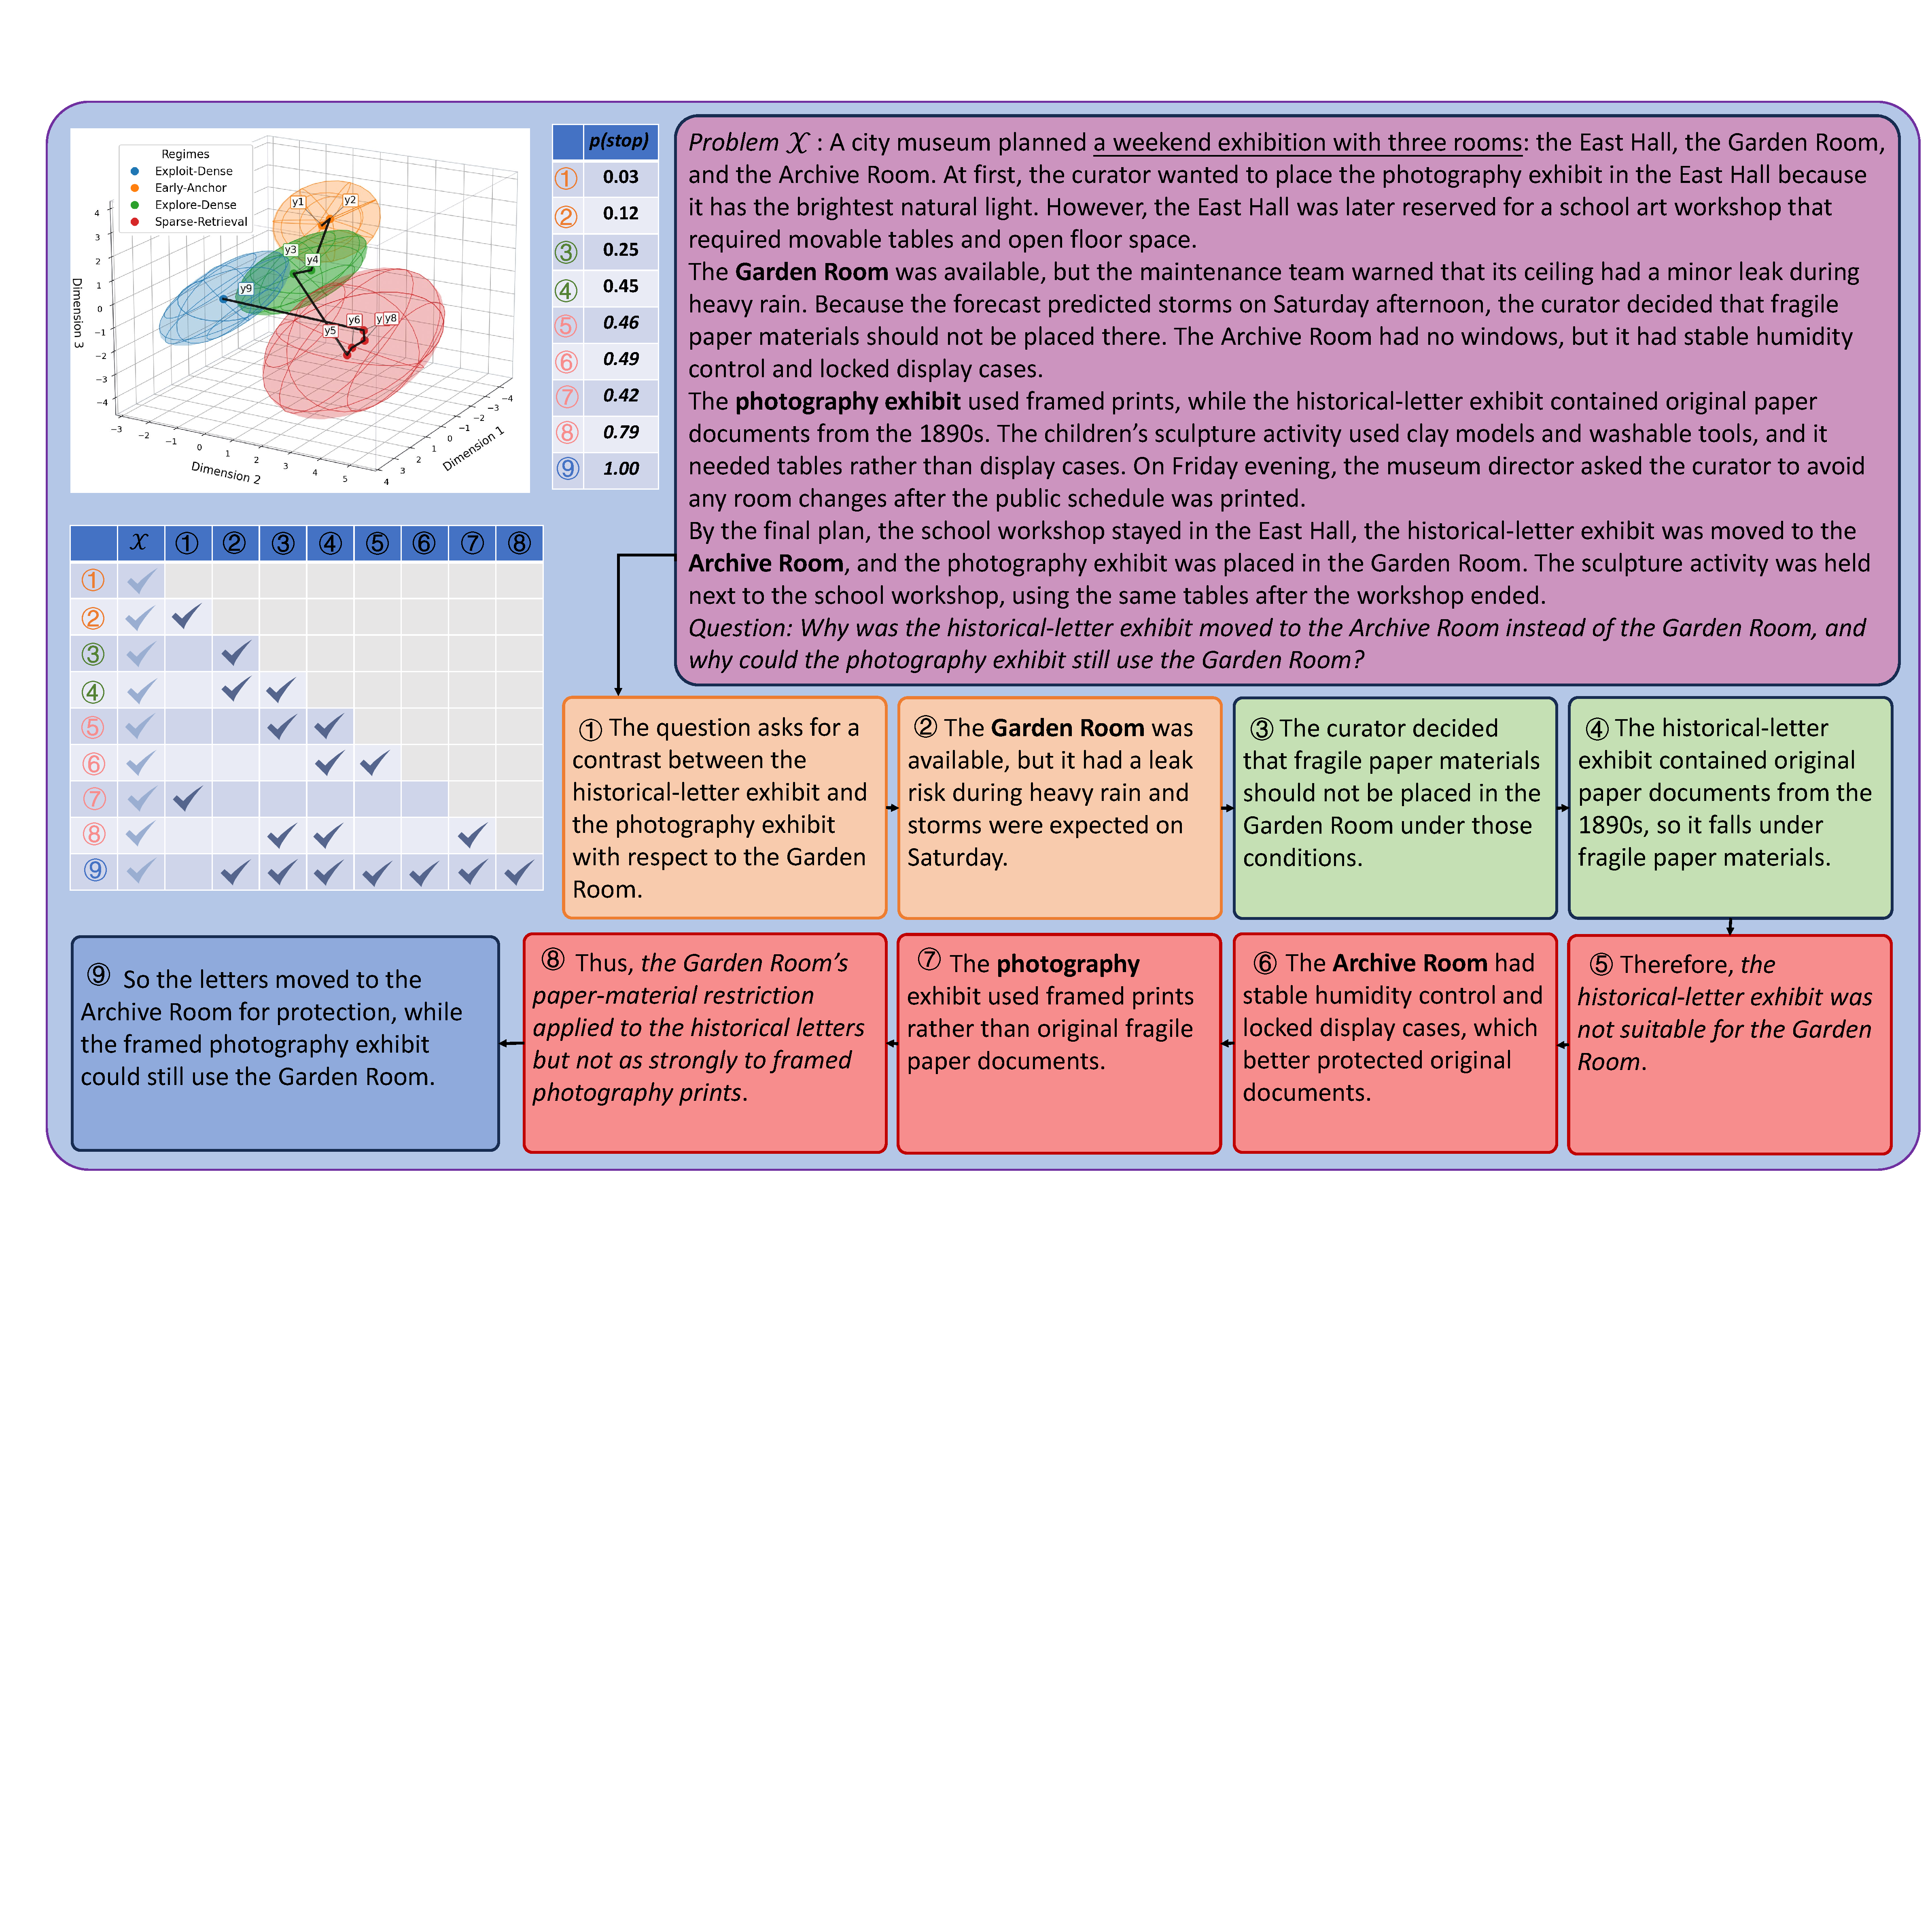
\includegraphics[width=0.98\textwidth]{figs/app_case_longcontext.pdf}
\vspace{-2mm}
\caption{Case study on Long-Context Reasoning (LCR).}
\label{fig:app_case_longcontext}
\end{figure}

\subsection{Case 5: Visual-language reasoning}
\vspace{-1mm}
Figure~\ref{fig:app_case_vlm} (Qwen3-VL-8B) shows the same interface on chart QA: panel-wise extraction, numeric gap reasoning, rising \(p(\mathrm{stop})\) through the computation, and sparse dependencies—evidence that SoT remains a trajectory-level organizer when evidence is grounded in pixels rather than text alone.
\vspace{-3mm}

\begin{figure}[H]
\centering
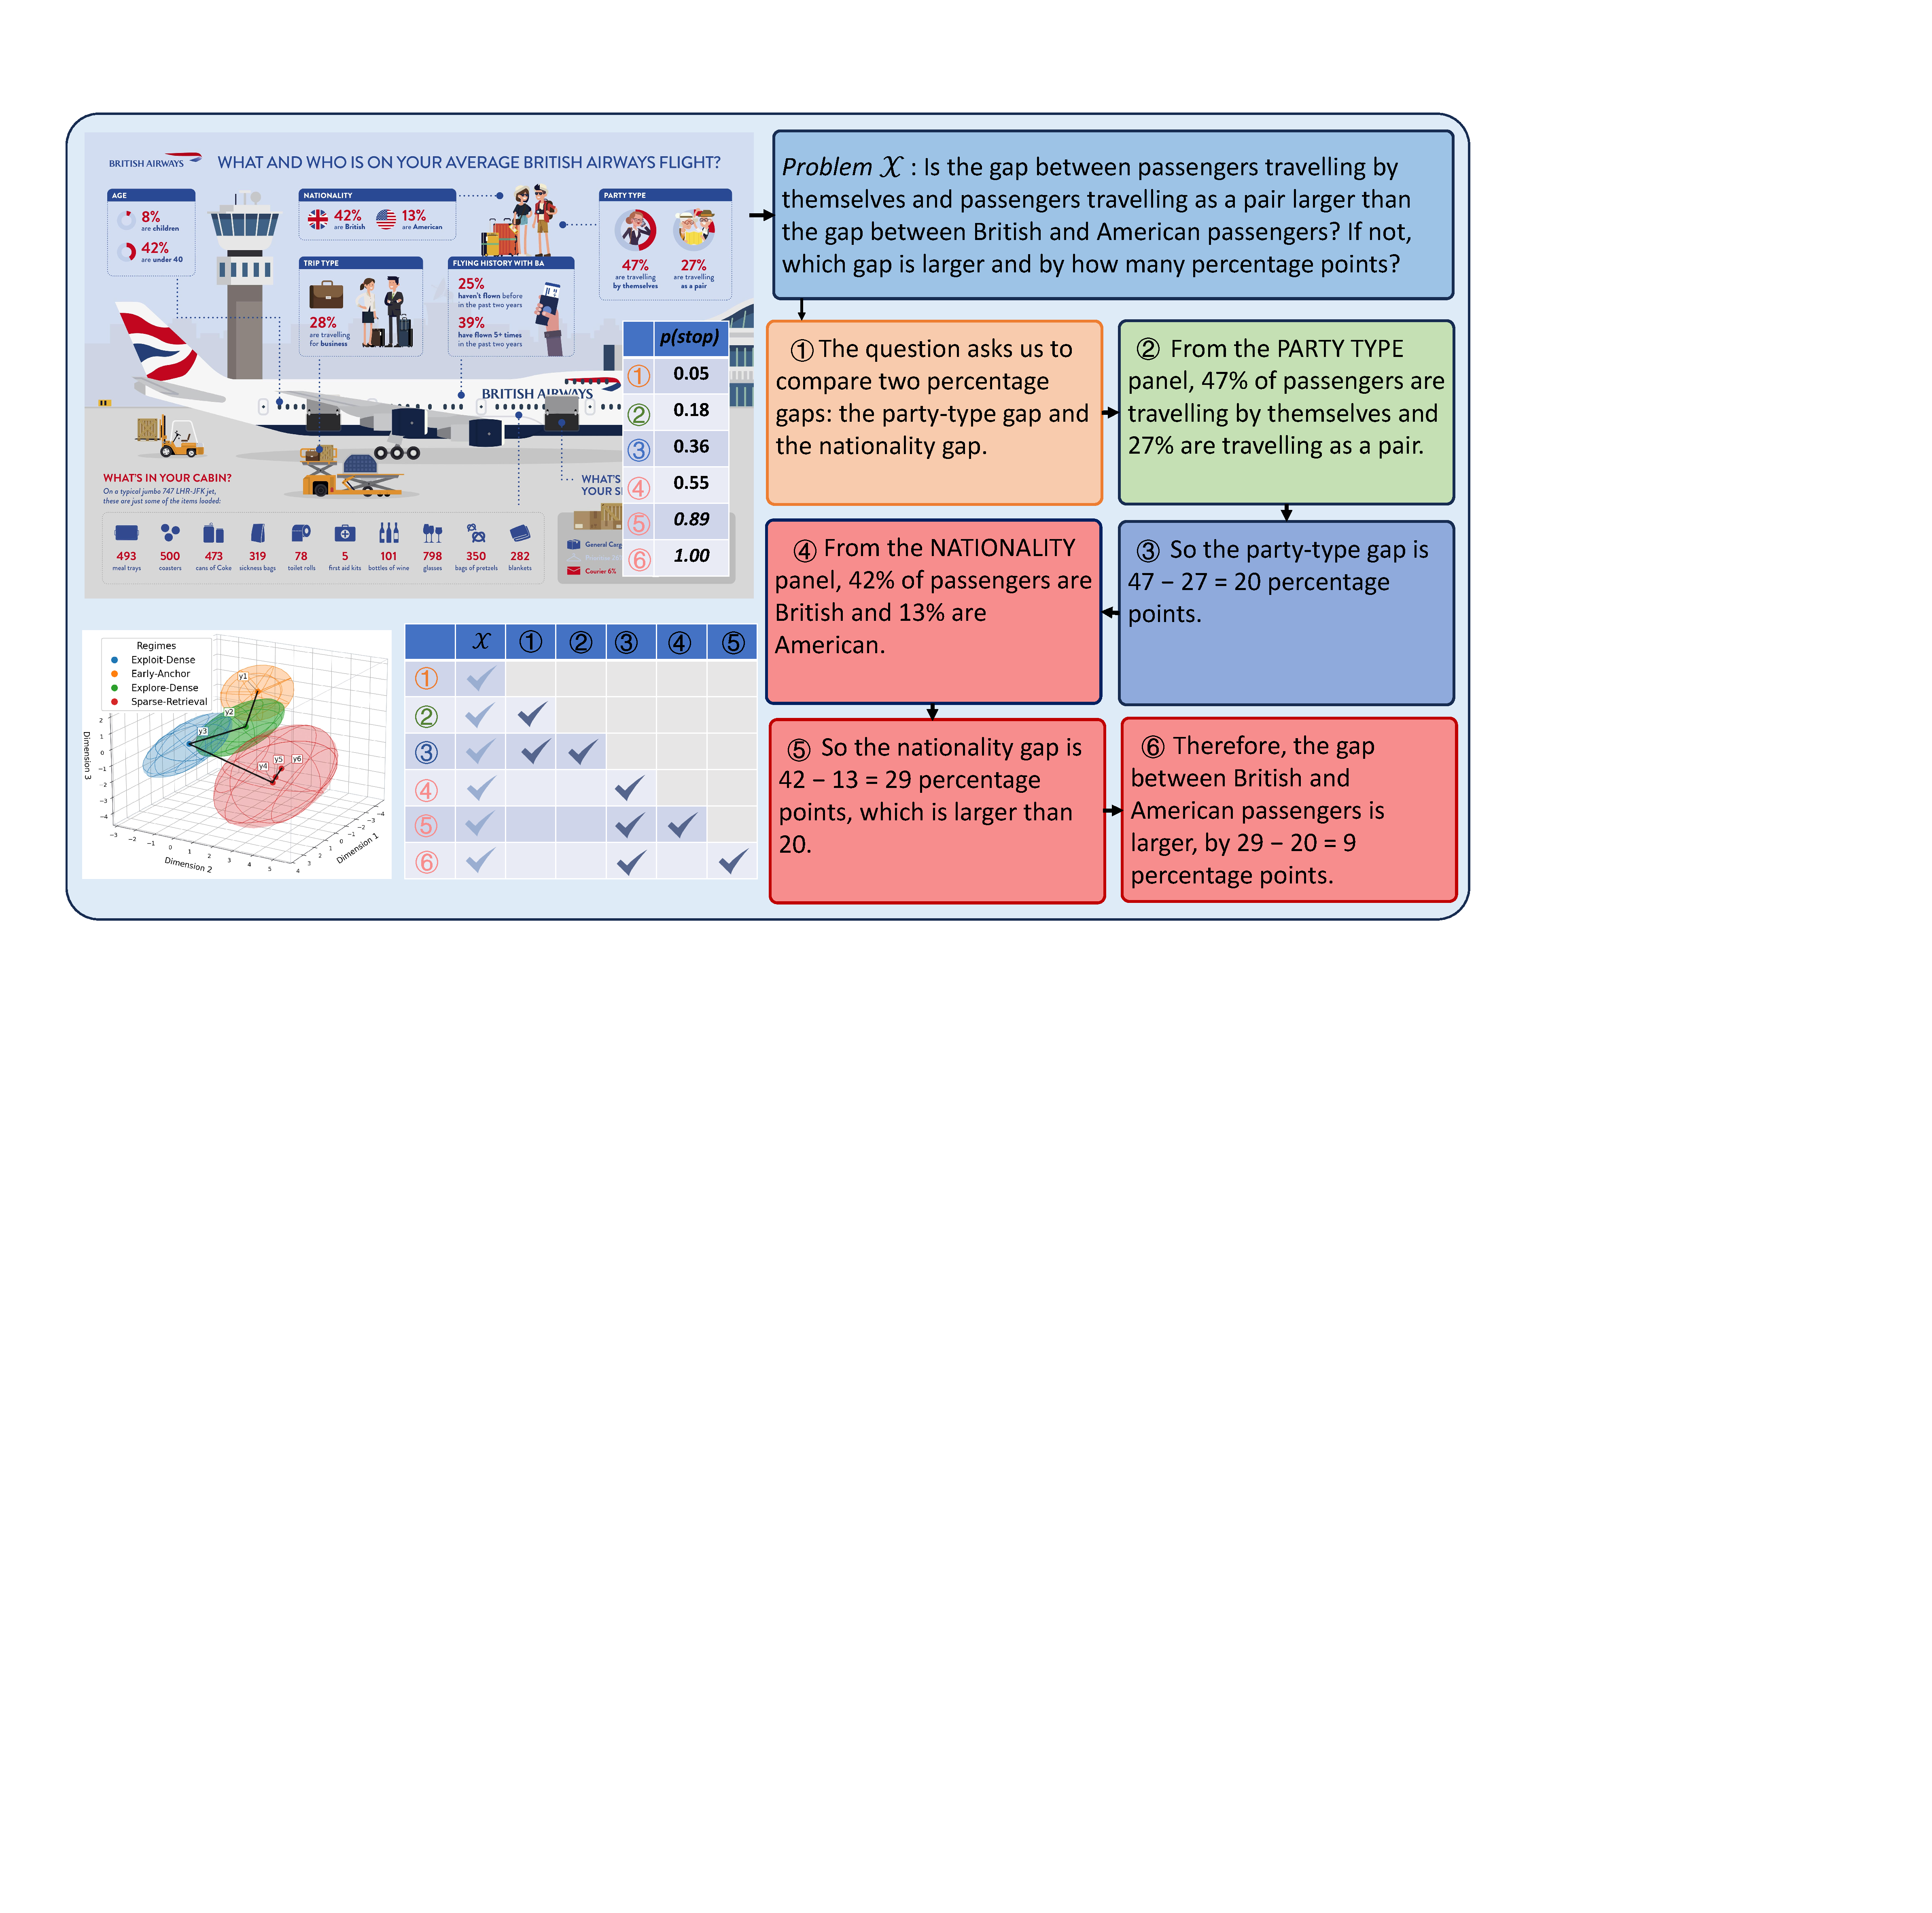
\includegraphics[width=0.98\textwidth]{figs/app_case_vlm.pdf}
\vspace{-2mm}
\caption{Case study on visual-language reasoning.}
\label{fig:app_case_vlm}
\end{figure}

% =========================================================
% Part E: Related Work and Discussion
% =========================================================
\clearpage
\AppBlock{Part E: Related Work and Discussion}
\vspace{-2mm}

\section{Related Work}
\label{app:related_work}
\vspace{-1mm}

This section expands the compressed related-work discussion from the main paper.
SoT sits at the intersection of four research directions, but is not reducible to any one of them.
\vspace{-1mm}

\subsection{Externally scripted reasoning}
\vspace{-1mm}
One major line of work improves reasoning by imposing explicit inference-time structure:
step-by-step prompting~\citep{wei2022chain},
self-consistency~\citep{wang2023selfconsistency},
plan-and-solve decomposition~\citep{wang2023plan},
self-refinement~\citep{madaan2023self},
and tree-style search~\citep{yao2023tree}.
These methods substantially advance empirical reasoning performance, but they share a common modeling assumption:
reasoning improves when we prescribe a better \emph{external} program for how the model should think.

SoT differs at the level of problem formulation.
It does not ask for a better externally specified chain.
It asks whether the model's current endogenous regime can decide what evidence should remain active for the next decision.
In this sense, SoT shifts the focus from \emph{external reasoning choreography} to \emph{endogenous reasoning control}.

\vspace{-1mm}
\subsection{Internal reasoning trajectories}
\vspace{-1mm}
Another relevant line studies hidden-state geometry, representation dynamics, and correctness-related trajectory structure in language models~\citep{ballon2026probing,damirchi2026truth,park2025geometry,park2024linear,sun2026llm}.
Related work also shows that internal signals can support monitoring and early-exit decisions~\citep{feng2025monitoring,hosseini2026early,tikhonov2026confidence}.
These works motivate the view that reasoning-relevant structure exists inside the model.

However, most of this literature is primarily descriptive:
it interprets hidden trajectories, monitors confidence, or probes latent variables.
SoT draws on similar geometric-dynamic structure but uses it differently.
Rather than analyzing the state after the fact, SoT engages it online as the control variable that determines evidence organization and continuation.

\vspace{-1mm}
\subsection{Context augmentation and compression}
\vspace{-1mm}
Retrieval-augmented and context-management methods also intersect with SoT.
Examples include retrieval-interleaved reasoning~\citep{trivedi2023interleaving,wang2024rat}, context compression~\citep{jiang2024longllmlingua,li2023compressing}, and KV-cache or memory-selection methods such as H\(_2\)O, SnapKV, and StreamingLLM~\citep{li2024snapkv,xiao2023streamingllm,zhang2023h2o}.
These methods are close to SoT in execution form because they do not always carry the entire history forward.

The key distinction lies in \emph{what drives selection}.
Most prior methods rely on semantic relevance, recency, generic compression objectives, or infrastructure efficiency.
SoT instead conditions historical activation on the model's current reasoning regime.
This turns memory selection from a general context-management tool into a component of reasoning control itself.

\vspace{-1mm}
\subsection{Latent reasoning and test-time control}
\vspace{-1mm}
Recent work also explores reasoning in latent space or with alternative test-time control ~\citep{hao2025training,hassid2025dont,wang2025system}.
Some methods push more reasoning inside hidden computation; others show that shorter or differently allocated reasoning traces can be beneficial.
These directions are highly relevant because they challenge the naive idea that better reasoning must always mean longer explicit token chains.

SoT is complementary to this line.
It does not replace explicit reasoning with a fully latent process, nor does it merely shorten chains.
Instead, it treats explicit sentence-level reasoning as a trajectory whose supporting context should be routed by a compact endogenous controller.
This makes SoT a bridge between explicit-token and latent-control views of reasoning.

\vspace{-1mm}
\subsection{Positioning summary}
\vspace{-1mm}
Overall, SoT should not be read as another CoT variant, another search baseline, or another memory-pruning heuristic.
Its central contribution is to formulate reasoning-time control as a closed loop in which endogenous state governs sparse evidence activation and stopping.
That is a different object of study from externally scripted reasoning, descriptive hidden-state analysis, or generic context compression.

\section{Limitations and Future Work}
\label{app:limitations_future}

This paper focuses on a concrete instantiation of SoT across multiple text backbones and one multimodal backbone; several scope boundaries naturally remain.
From a broader-impact perspective, improving reasoning under fixed inference budgets could make capable models more usable in cost- or latency-sensitive settings (e.g., education, healthcare-related assistance, research tooling), where efficiency and reliability both matter.
As with any method that can improve fluent reasoning, deployment should follow domain-appropriate safeguards (e.g., policy constraints, human oversight in high-stakes use, and monitoring for misuse).

\subsection{Current limitations}
\begin{itemize}[leftmargin=1.6em]
    \item \textbf{Performance depends on the state interface.}
    SoT routes memory and stopping through the extracted endogenous state; if that interface is a poor summary of the regime relevant to the next decision, control quality can degrade.

    \item \textbf{The current state is intentionally compact.}
    Our implemented controller uses \(m_t\in\mathbb{R}^{4}\) for clarity and portability, but this choice may under-specify unusually long, highly branching, or richly grounded trajectories where additional structure could help.

    \item \textbf{Mechanistic evidence is supportive but not uniquely identifying.}
    Our ablations and interventions are consistent with state-conditioned routing playing a central role, yet---as in most systems that couple representation, memory, and generation---alternative narratives cannot be ruled out in every corner case without heavier instrumentation.

    \item \textbf{Empirical coverage matches the paper's claims, not every deployment regime.}
    We report results across a broad multi-task suite, but stronger proprietary models, different tool-use/agent stacks, and safety-critical deployments are outside our evaluated scope.

    \item \textbf{Limited-access variants are informative but not exhaustive.}
    Training-free SoT, embedding-based features, and \textsc{SoT-Judge} probe the same interface under restricted supervision or observability; they are evaluated at a smaller footprint than the full supervised controller and are best read as exploratory complements.
\end{itemize}

\subsection{Future work}
\begin{itemize}[leftmargin=1.6em]
    \item \textbf{Richer but still compact states.}
    A natural direction is to add state dimensions or structured summaries only when they measurably improve control (e.g., branching, retrieval confidence, multimodal grounding), without bloating the feedback loop.

    \item \textbf{Tighter identification of what the controller uses.}
    Additional counterfactual replay, routing interventions, and closed-loop stress tests could further clarify which components of the interface matter most across task families.

    \item \textbf{Adaptive memory units.}
    Sentence-level units are easy to audit, but variable segmentation or hybrid symbolic/latent memories may better match heterogeneous reasoning traces.

    \item \textbf{Unified white-box and black-box trajectory control.}
    SoT-Embed and \textsc{SoT-Judge} suggest a continuum between internals-aware controllers and trajectory-only signals; a more systematic comparison of that continuum is an interesting next step.

    \item \textbf{Broader multimodal and interactive settings.}
    Environments with dynamic evidence---long multimodal contexts, tool use, and interactive decisions---are a natural fit for state-conditioned organization, but will require task suites and training protocols beyond this paper.
\end{itemize}

\paragraph{Final perspective.}
We intend SoT as a precise formulation of reasoning-time control---not a claim that any single architecture is final.
The underlying point is empirical and conceptual: reasoning benefits from treating context activation and continuation as a feedback process coupled to the model's evolving internal regime, rather than only as prompt programming over a growing transcript.
